\subsubsection{Modellentwicklung am Objekt}\label{hw_case_modellentwicklung}
\paragraph{Grundskizze}\\
\noindent Nachdem das Testmodell (vgl. Abb. \ref{fig:print-case-test_04}: \nameref{fig:print-case-test_04}) nicht zu 100 \% gepasst hat, haben wir die Abmessungen neu erfasst und diese in Fusion 360 übertragen (vgl. Abb. \ref{fig:case_footprint}: \nameref{fig:case_footprint}). 
Um Material für den 3D-Druck zu sparen, haben wir eine Papierschablone erstellt, die Zeichnung dann im Maßstab 1:1 auf Papier ausgedruckt, ausgeschnitten und am Bildschirm angelegt.\par
\noindent So haben wir die Maße angepasst und den Plan entsprechend ergänzt(vgl. Abb. \ref{fig:case_footprint_final}: \nameref{fig:case_footprint_final}).\\
\noindent Die Zeichnung haben wir in zwei eigenständige Dateien gesplittet, um die linke und die rechte Seite des Gehäuses konstruieren zu können.\par
\noindent Die Grundabmessung des Bildschirms haben wir in Fusion 360 als neue Zeichnung angelegt. 
Hierzu haben wir ein einfaches Rechteck mit den entsprechenden Außenmaßen gezeichnet (vlg. Abb. \ref{fig:design-case-01}: \nameref{fig:design-case-01}) und anschließend die Ecken mit einem Radius von 7 mm abgerundet (vgl. Abb. \ref{fig:design-case-02}: \nameref{fig:design-case-02}). 
Die Zeichnung haben wir in der Mitte geteilt, um die beiden Hälften des Gehäuses unabhängig von einander konstruieren zu können.\par
\begin{figure}[H]
	\begin{subfigure}[b]{.5\linewidth}
		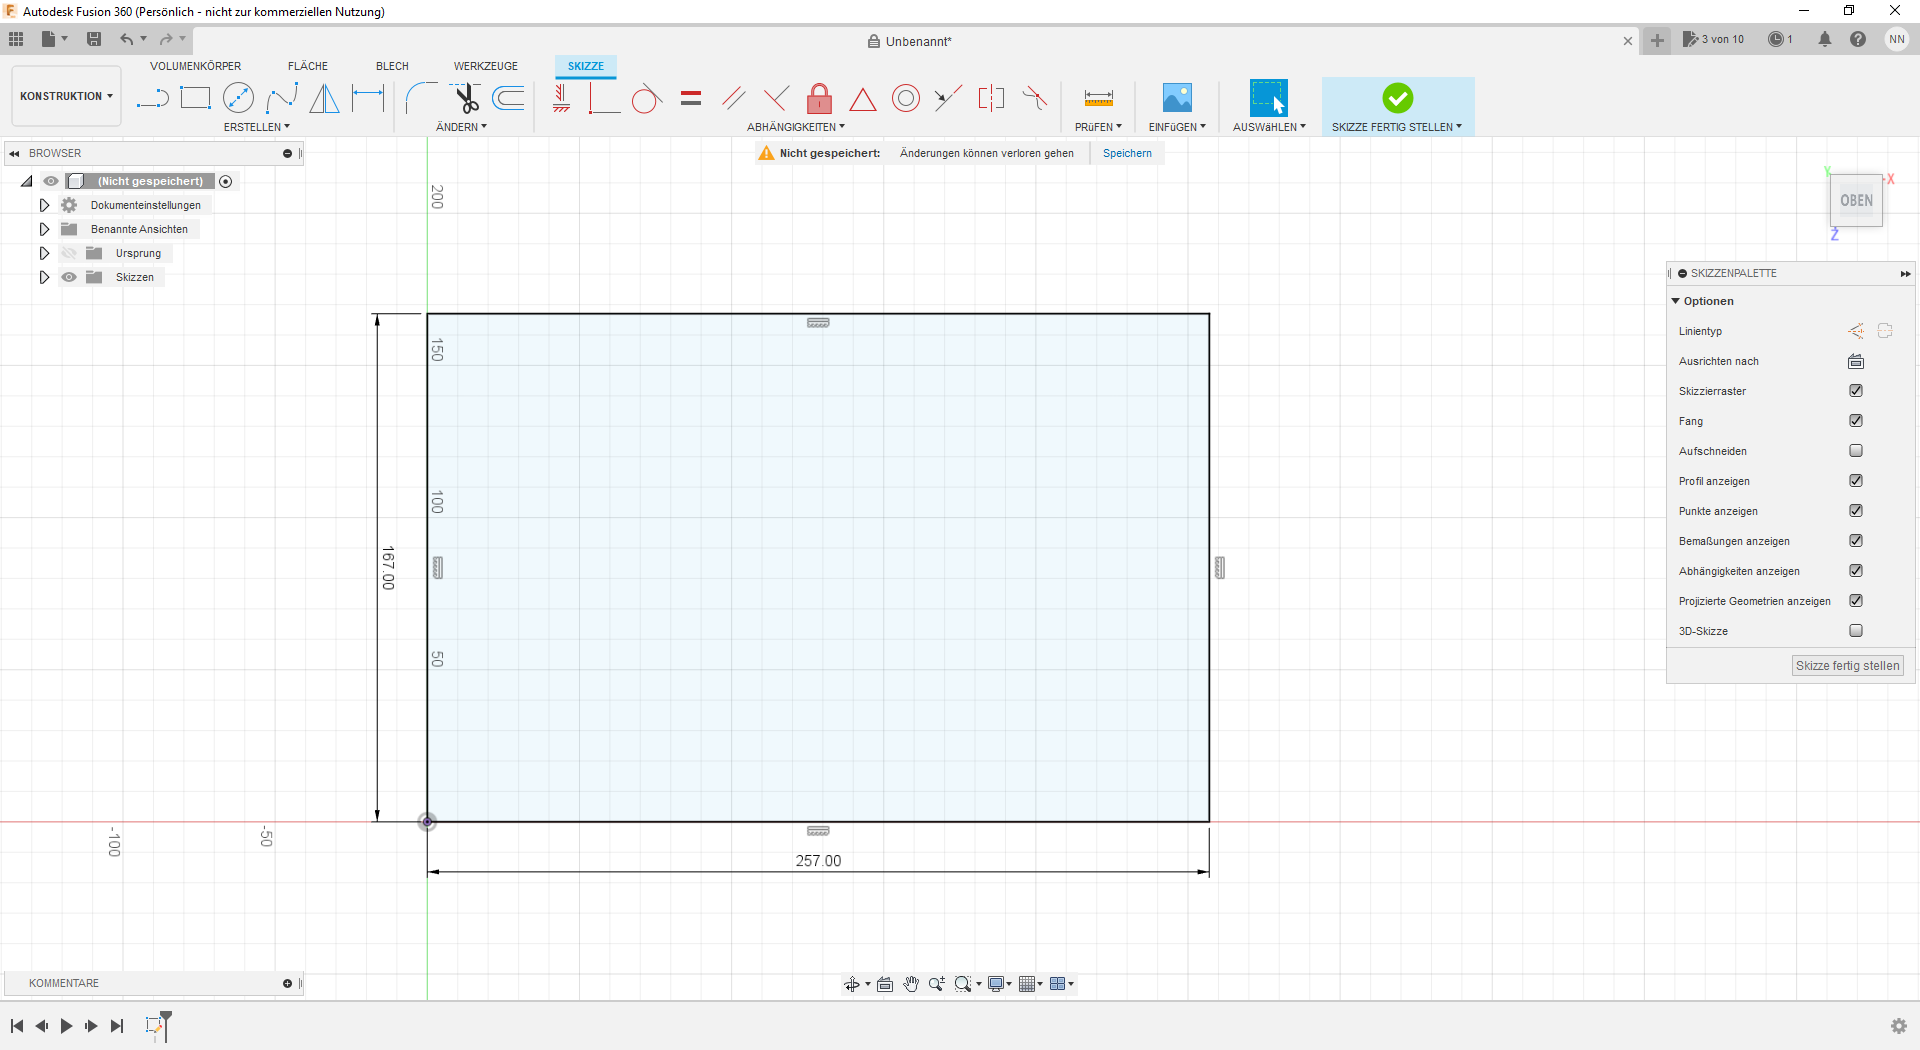
\includegraphics[width=1\textwidth]{img/konstruktion_gehaeuse_001.png}
		\caption[Zeichnen der Außenmaße]{Zeichnen der Außenmaße}
		\label{fig:design-case-01}
	\end{subfigure}
	\begin{subfigure}[b]{.5\linewidth}
		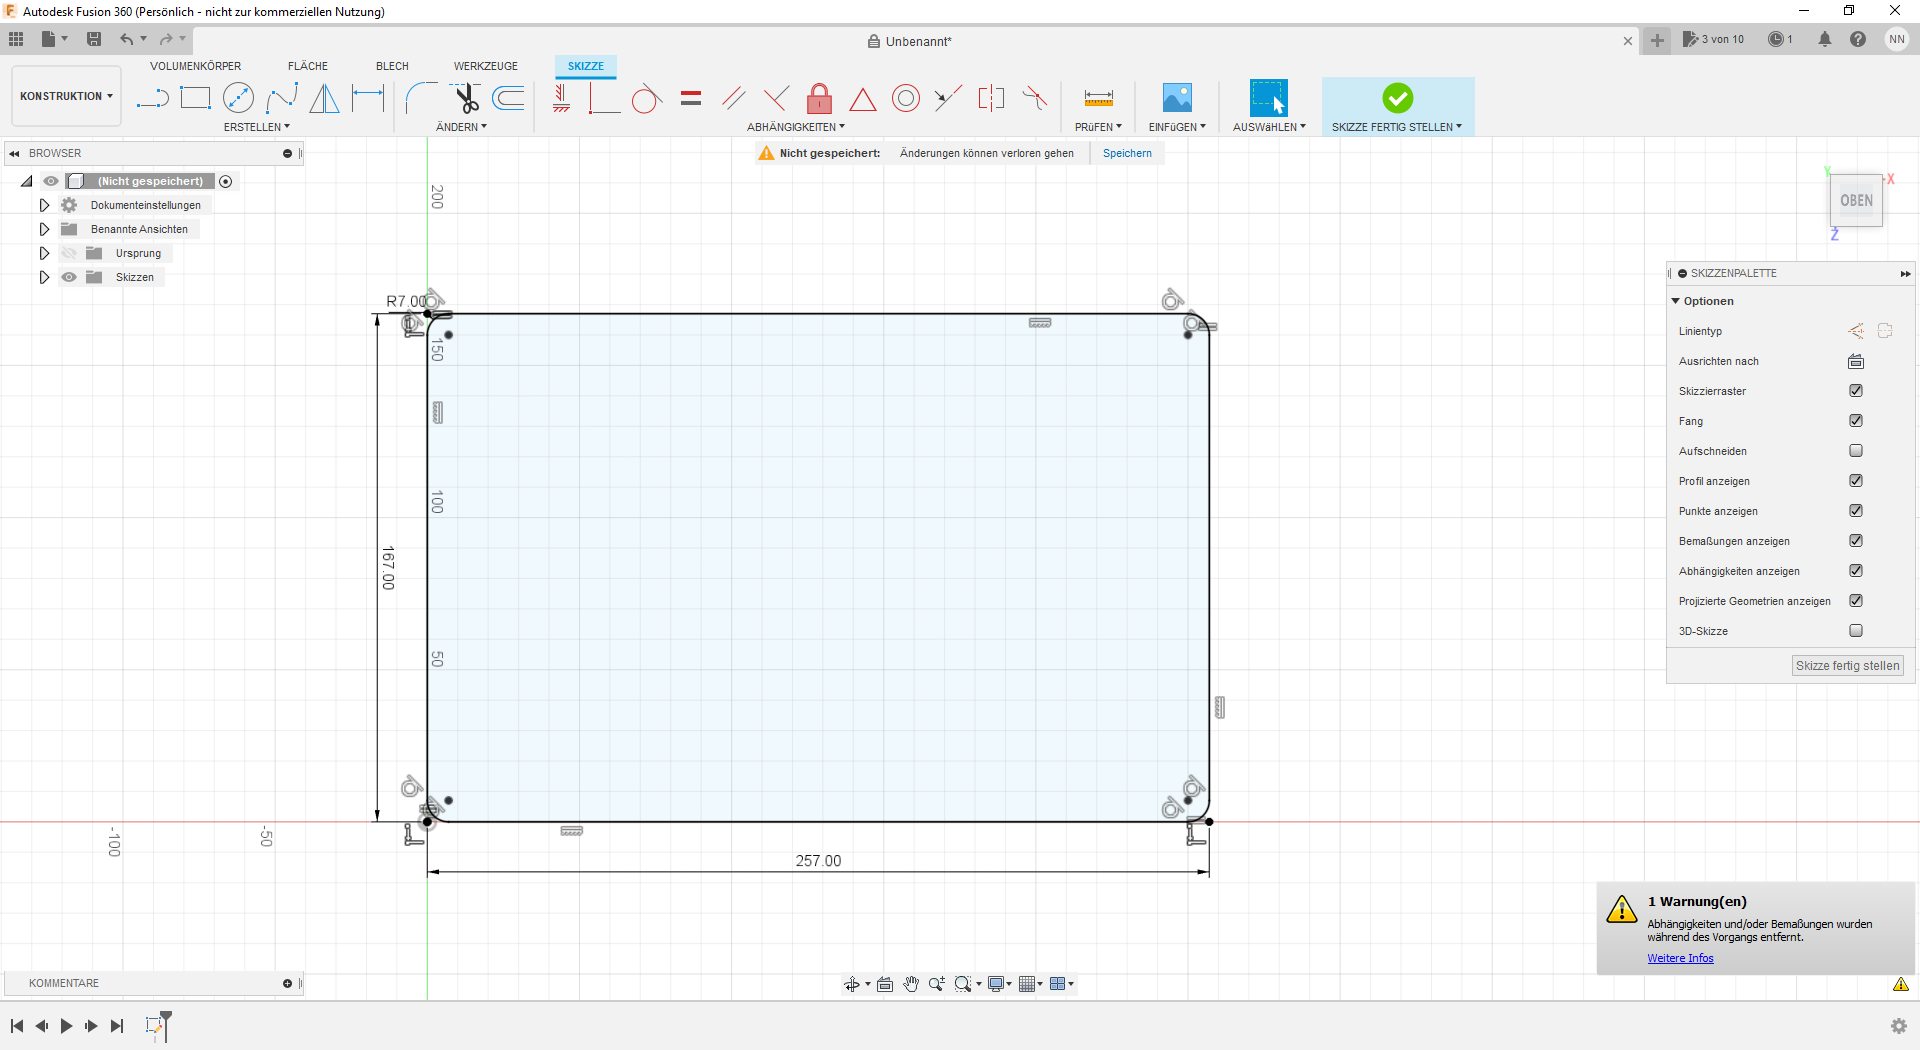
\includegraphics[width=1\textwidth]{img/konstruktion_gehaeuse_002.png}
		\caption[Abrunden der Ecken]{Abrunden der Ecken}
		\label{fig:design-case-02}
	\end{subfigure}
	\begin{subfigure}[b]{.5\linewidth}
		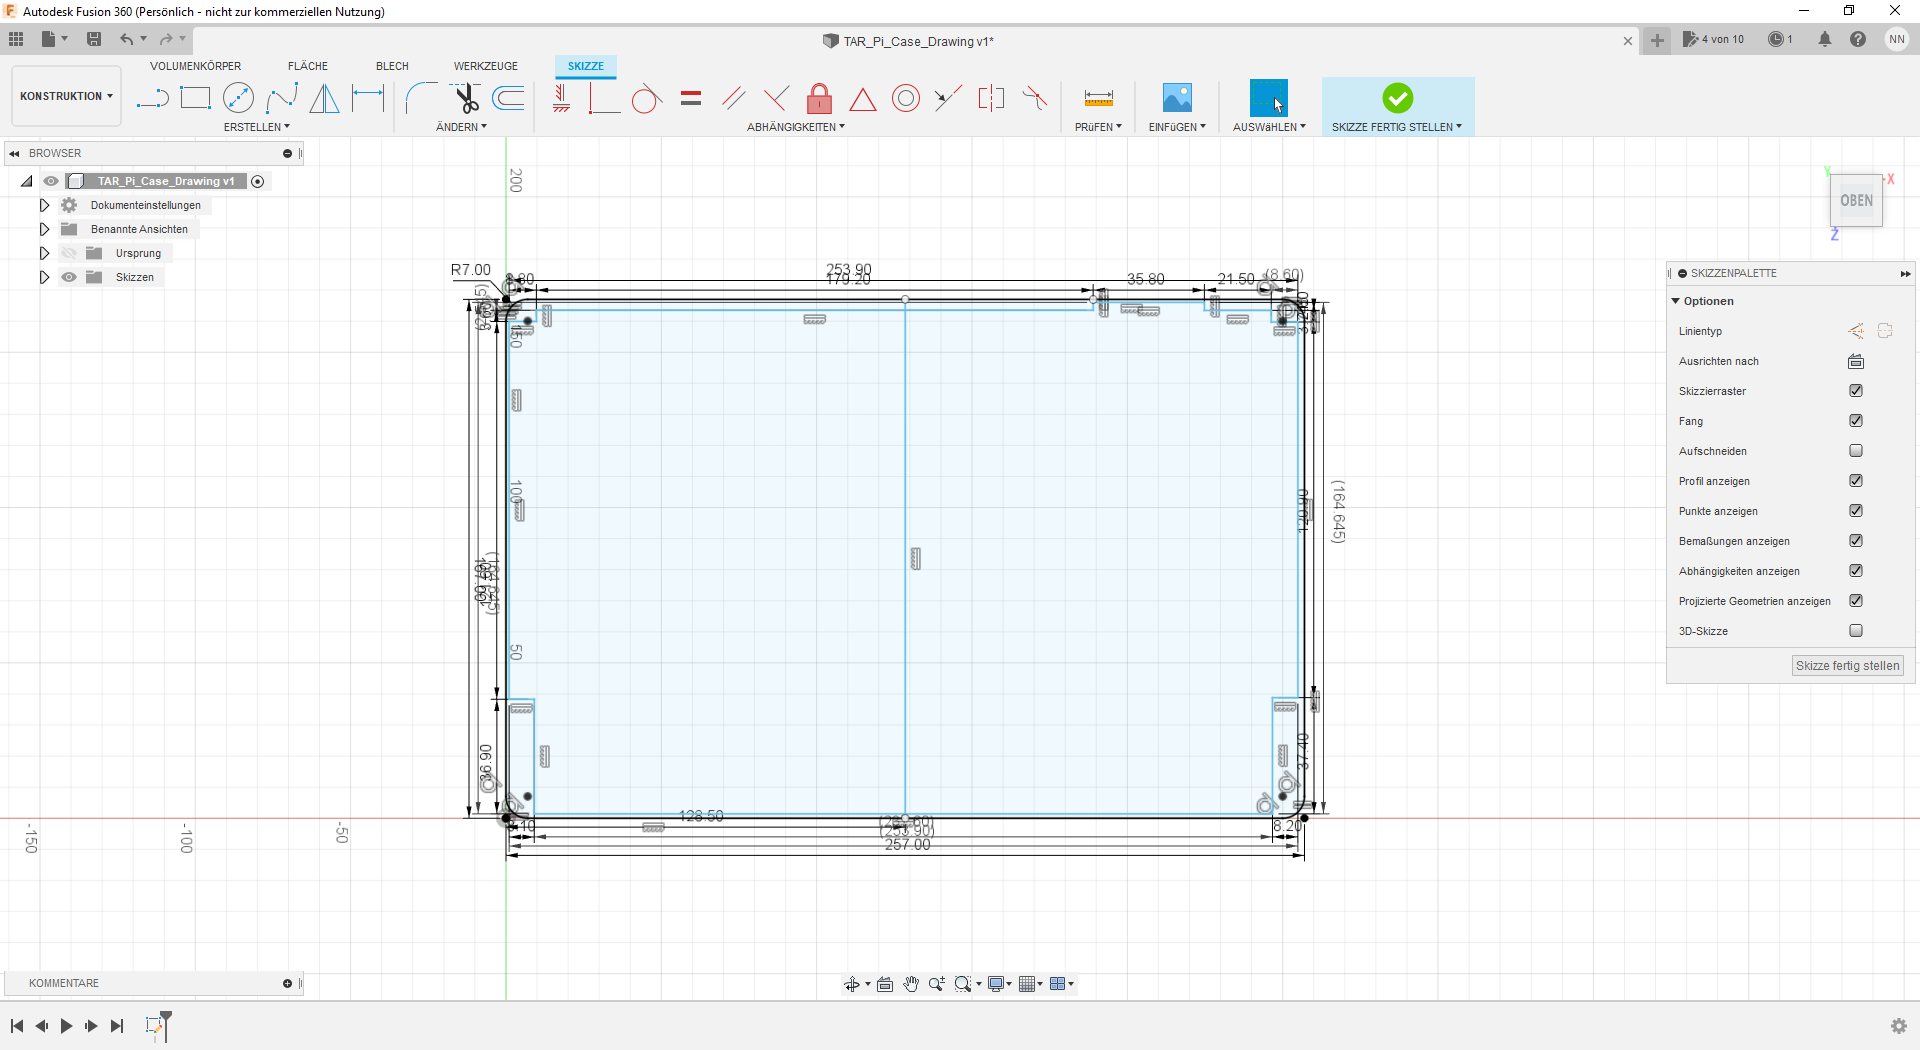
\includegraphics[width=1\textwidth]{img/konstruktion_gehaeuse_003.png}
		\caption[Zeichnen der Auflageflächen für das Gehäuse]{Zeichnen der Auflageflächen}
		\label{fig:design-case-03}
	\end{subfigure}
	\caption[Grundzeichnung als Basis des Modells]{Grundzeichnung als Basis des Modells}
	\label{fig:design-case-base}
\end{figure}\par
\noindent Die so entstandene Zeichnung (vgl. Abb. \ref{fig:design-case-03}: \nameref{fig:design-case-03}) haben wir dann in eine weitere Datei kopiert, die als Grundlage für die beide Seitenteile dient. 
Ausgehend von dieser Zeichnung aus haben wir die beiden Wandteile unabhängig voneinander entworfen.\par
\paragraph{Linkes Wandteil}
Beim linken Wandteil haben wir die Zeichnung um 2 mm entlang der Z-Achse nach oben extrudiert (vgl. Abb. \ref{fig:design-left-01}: \nameref{fig:design-left-01}), um eine Auflagefläche zu erzeugen. 
Auf der Oberseite haben wir eine weitere Zeichnung gelegt, um die Kontaktfläche für die Verklebung mit dem Bildschirm zu erweitern (vgl. Abb. \ref{fig:design-left-02}: \nameref{fig:design-left-02}), die wir dann wie zuvor um 3 mm entlang der Z-Achse extrudiert haben (vgl. Abb. \ref{fig:design-left-03}: \nameref{fig:design-left-03}) um auf die gleiche Höhe des Blechs auf der Rückseite des Bildschirms zu gelangen. \\
\noindent Diese sollte dem Gehäuse genug Auflagefläche auf dem Bildschirm bieten, um die Verklebung so stabil wie möglich zu machen. 
Auf die nun entstandene Erhöhung haben wir eine Zeichnung des Rahmens von 3 mm Stärke erstellt (vgl. Abb. \ref{fig:design-left-04}: \nameref{fig:design-left-04}), die wir dann um 6 mm entlang der Z-Achse extrudiert haben, um für die Verbinder der Schrauben genügend Platz vor dem herausstehenden Blechbereich im unteren Teil des Bildschirms zu bieten (vgl. Abb.  \ref{fig:design-left-05}: \nameref{fig:design-left-05}). \\
\noindent Auf die nun obenliegende Seite des Gehäuses haben wir die Zeichnung der Verbindungsstücke gelegt (vgl. Abbildung \ref{fig:design-left-06}: \nameref{fig:design-left-06}), um 19 mm entlang der Z-Achse extrudiert (vgl. Abb. \ref{fig:design-left-07}: \nameref{fig:design-left-07}). 
Im Kreismittelpunkt der Zeichnungen eine Bohrung für M3-Gewinde gesetzt (vgl. Abb. \ref{fig:design-left-08}: \nameref{fig:design-left-08}). 
Auf die Oberseite haben wir die Zeichnung für die Verbindung von Deckel und dem Seitenteil gesetzt (vgl. Abb. \ref{fig:design-left-09}: \nameref{fig:design-left-09}) und um 25 mm entlang der Z-Achse extrudiert (vgl. Abb. \ref{fig:design-left-10}: \nameref{fig:design-left-10}), damit der von uns verwendete 40 mm Lüfter im Gehäuse Platz findet.
Dies haben wir ebenfalls mit Bohrungen für M3-Gewinde versehen (vgl. Abb. \ref{fig:design-left-11}: \nameref{fig:design-left-11}).\par
\begin{figure}[H]
	\begin{subfigure}[t]{.3\linewidth}
		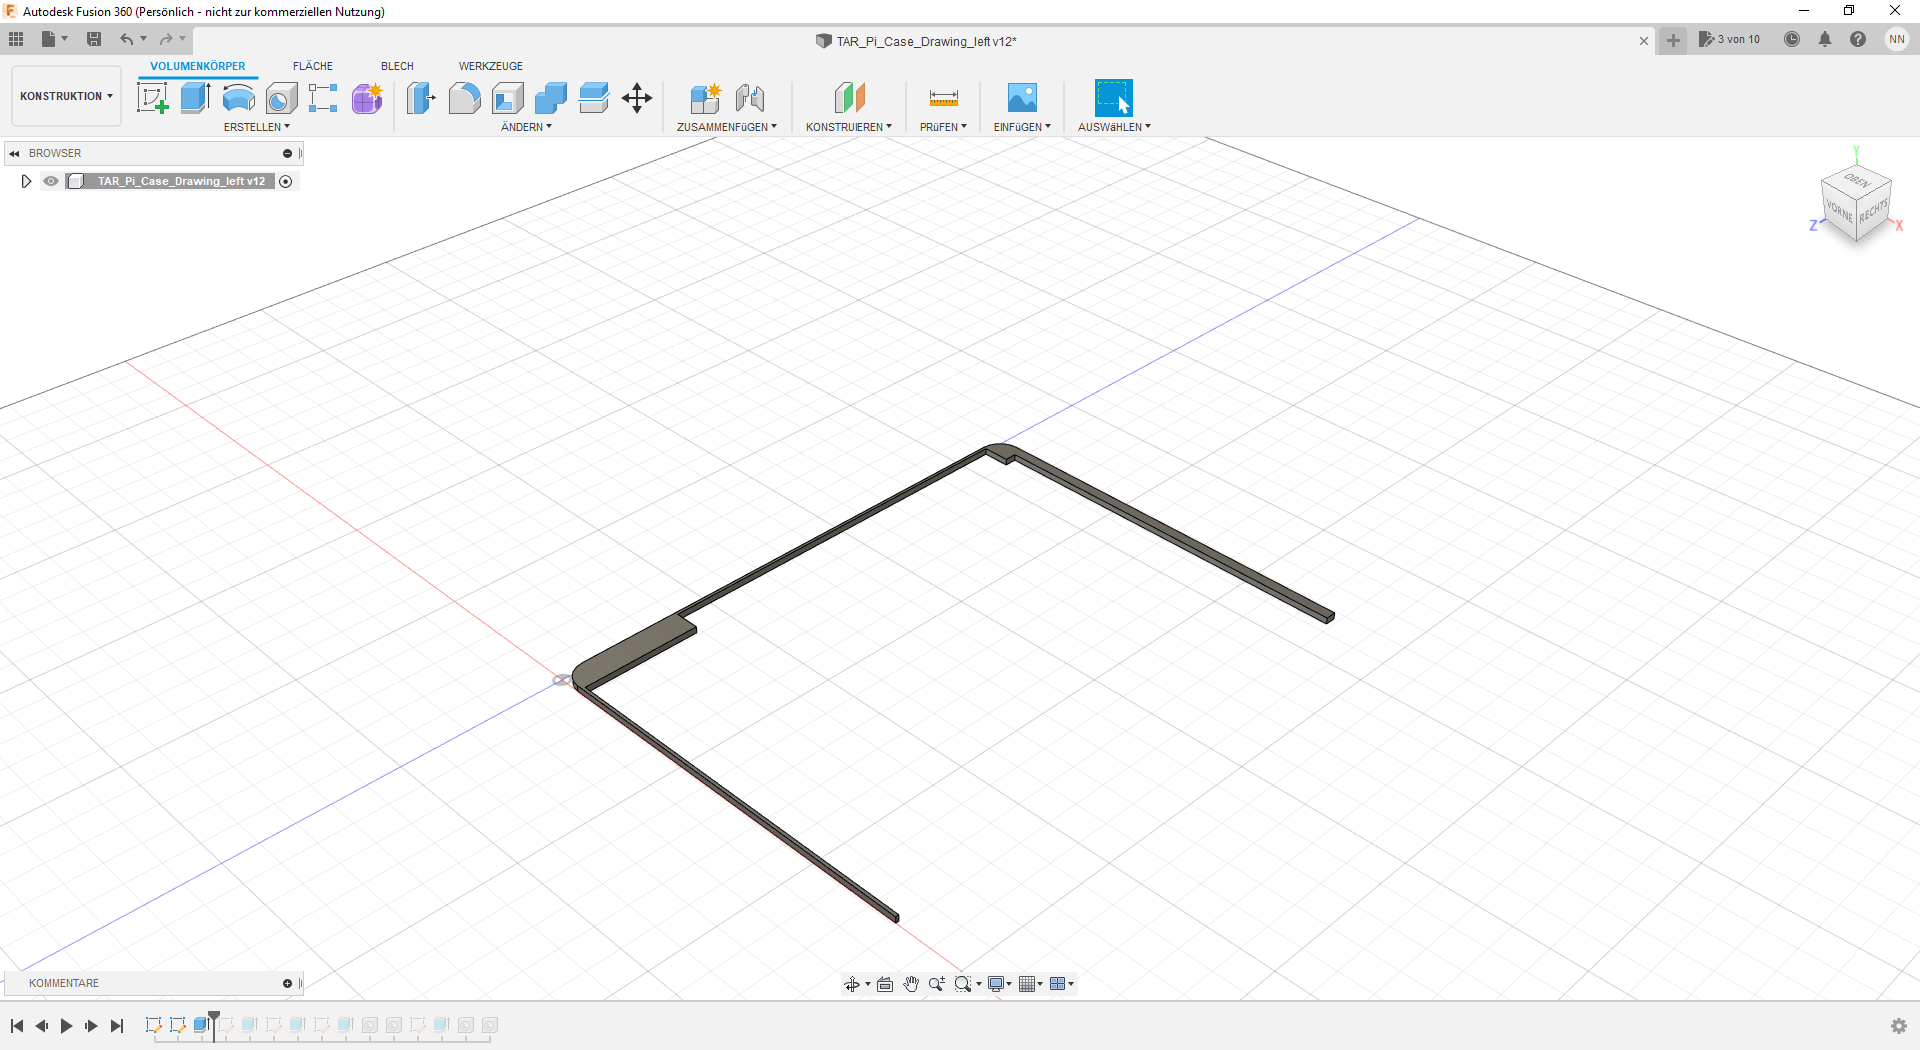
\includegraphics[width=\linewidth]{img/konstruktion_gehaeuse_links_001.png}
		\caption[Extrusion der Grundzeichnung]{Extrusion der Grundzeichnung}
		\label{fig:design-left-01}
	\end{subfigure}
	\begin{subfigure}[t]{.3\linewidth}
		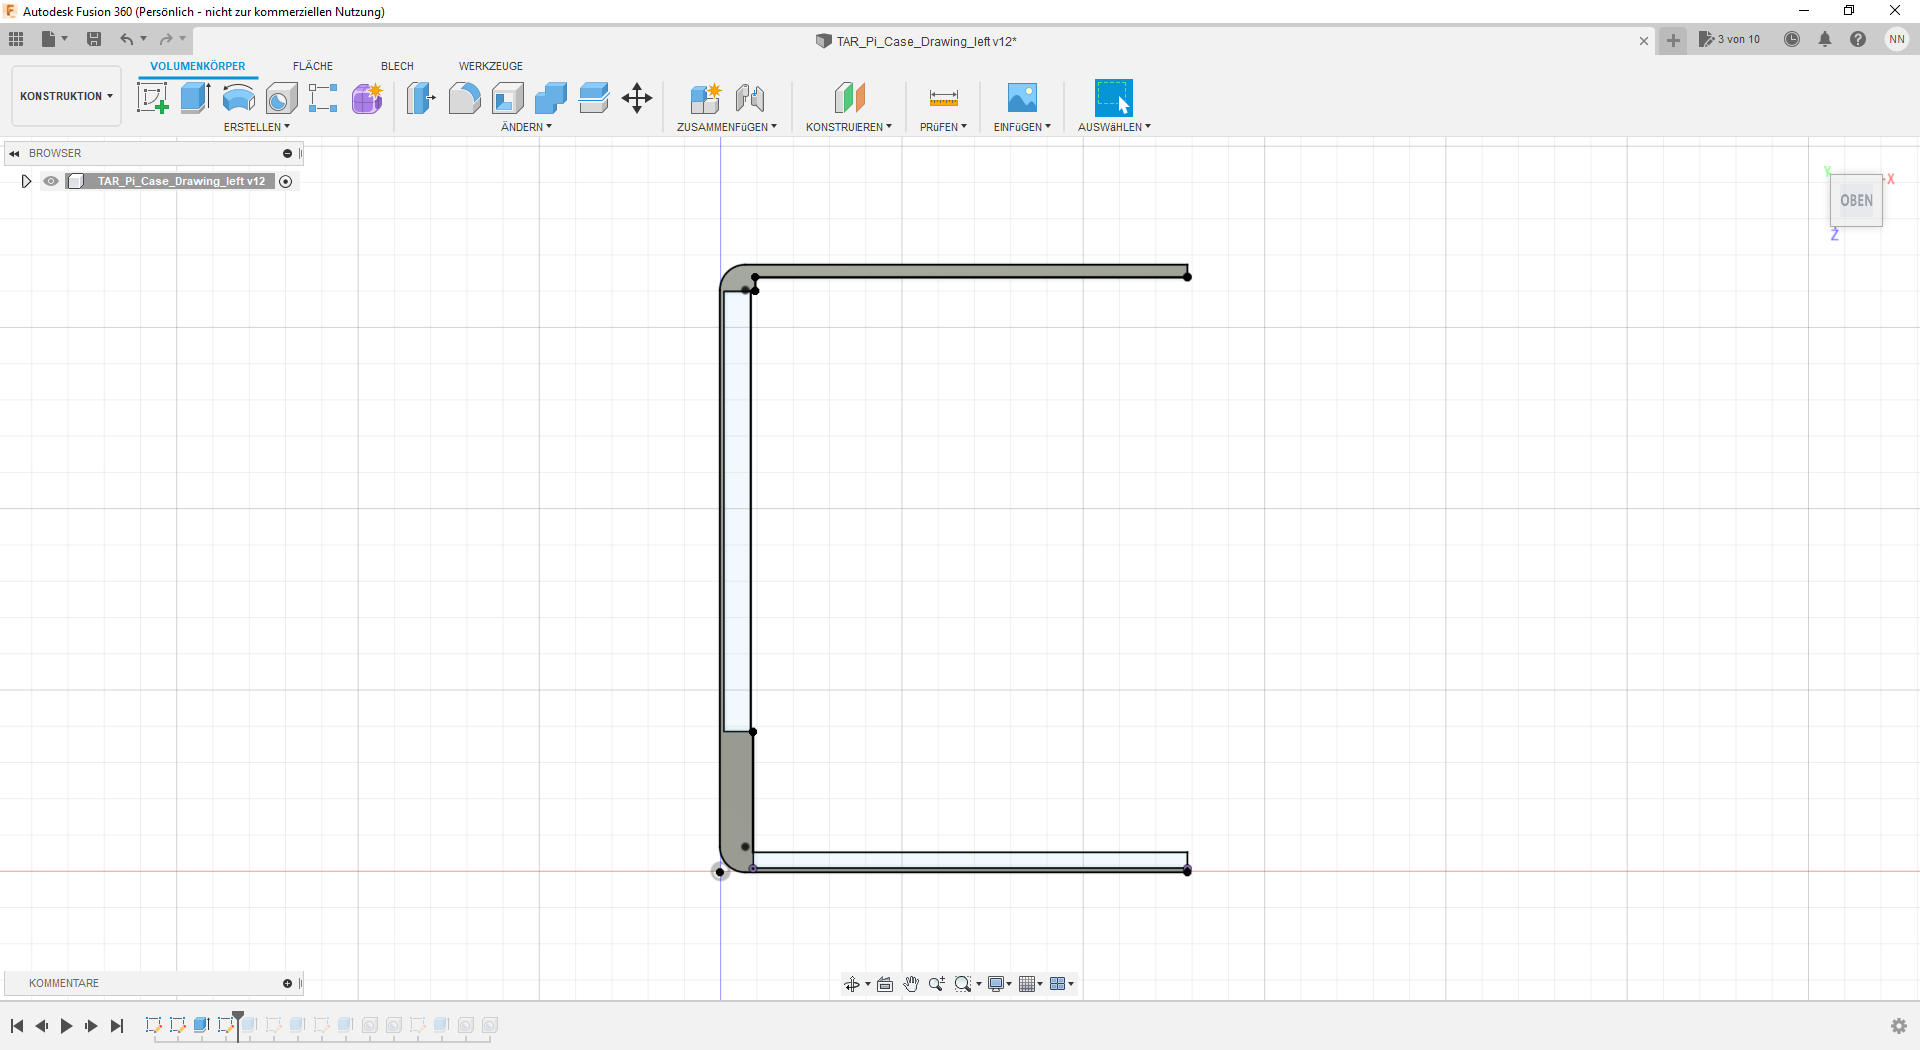
\includegraphics[width=\linewidth]{img/konstruktion_gehaeuse_links_002.png}
		\caption[Erstellung der Folgezeichnung um Blech]{Erstellung der Folgezeichnung um Blech}
		\label{fig:design-left-02}
	\end{subfigure}
	\begin{subfigure}[t]{.3\linewidth}
		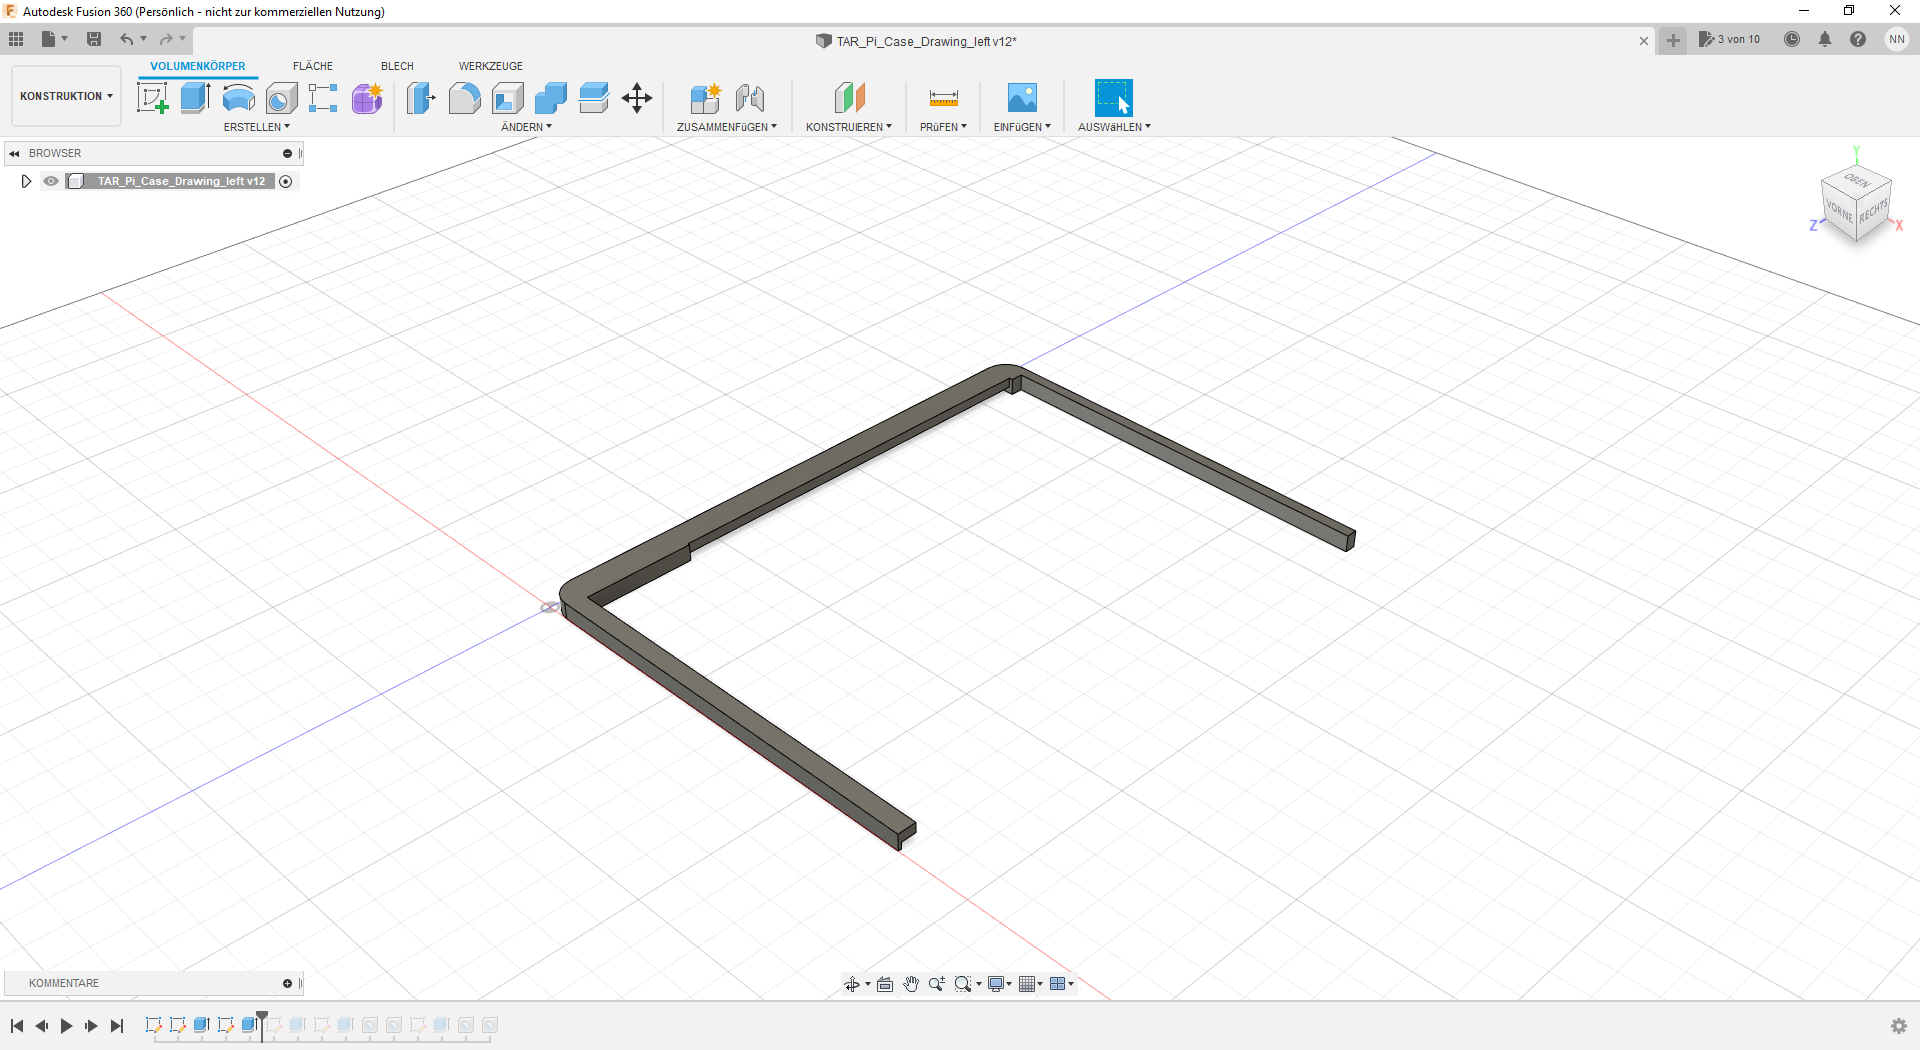
\includegraphics[width=\linewidth]{img/konstruktion_gehaeuse_links_003.png}
		\caption[Extrusion der neuen Zeichnung]{Extrusion der neuen Zeichnung}
		\label{fig:design-left-03}
	\end{subfigure}
	\begin{subfigure}[t]{.3\linewidth}
		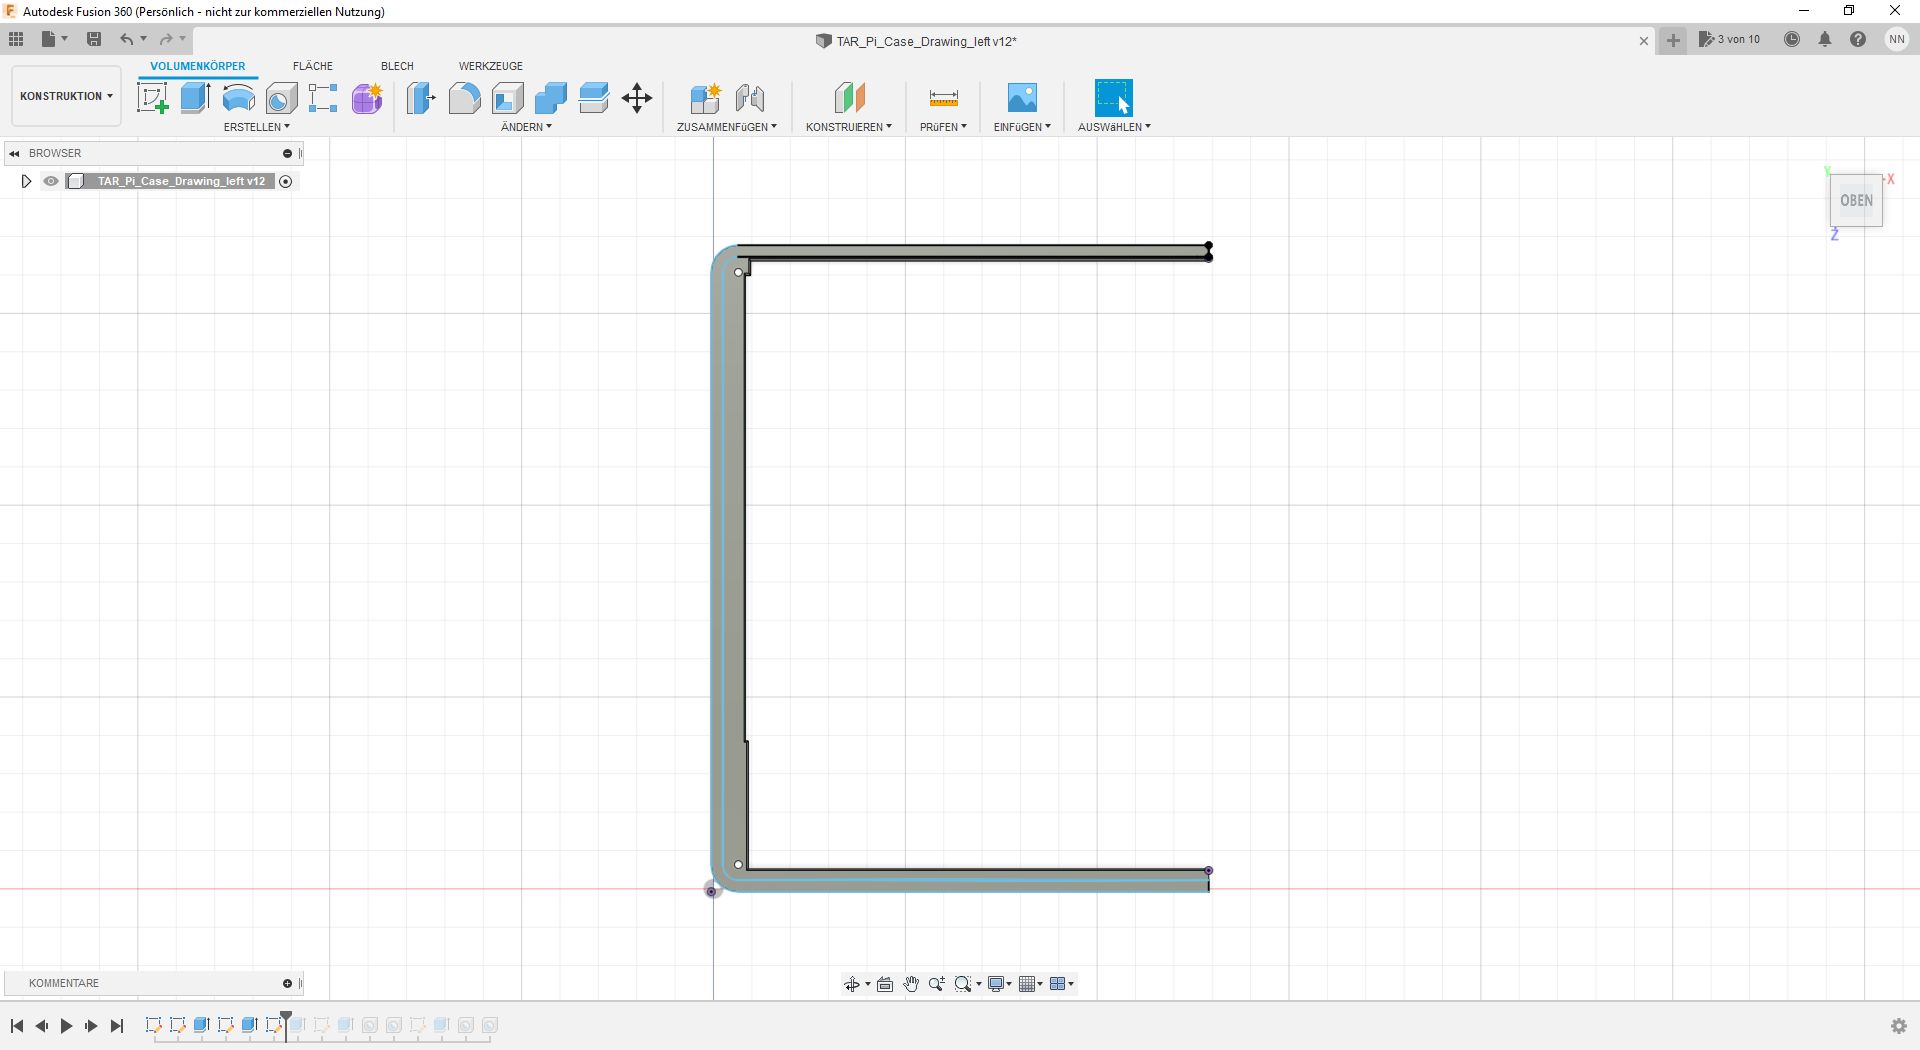
\includegraphics[width=\linewidth]{img/konstruktion_gehaeuse_links_004.png}
		\caption[Zeichnung der Hauptwandstärke]{Zeichnung der Hauptwandstärke}
		\label{fig:design-left-04}
	\end{subfigure}
	\begin{subfigure}[t]{.3\linewidth}
		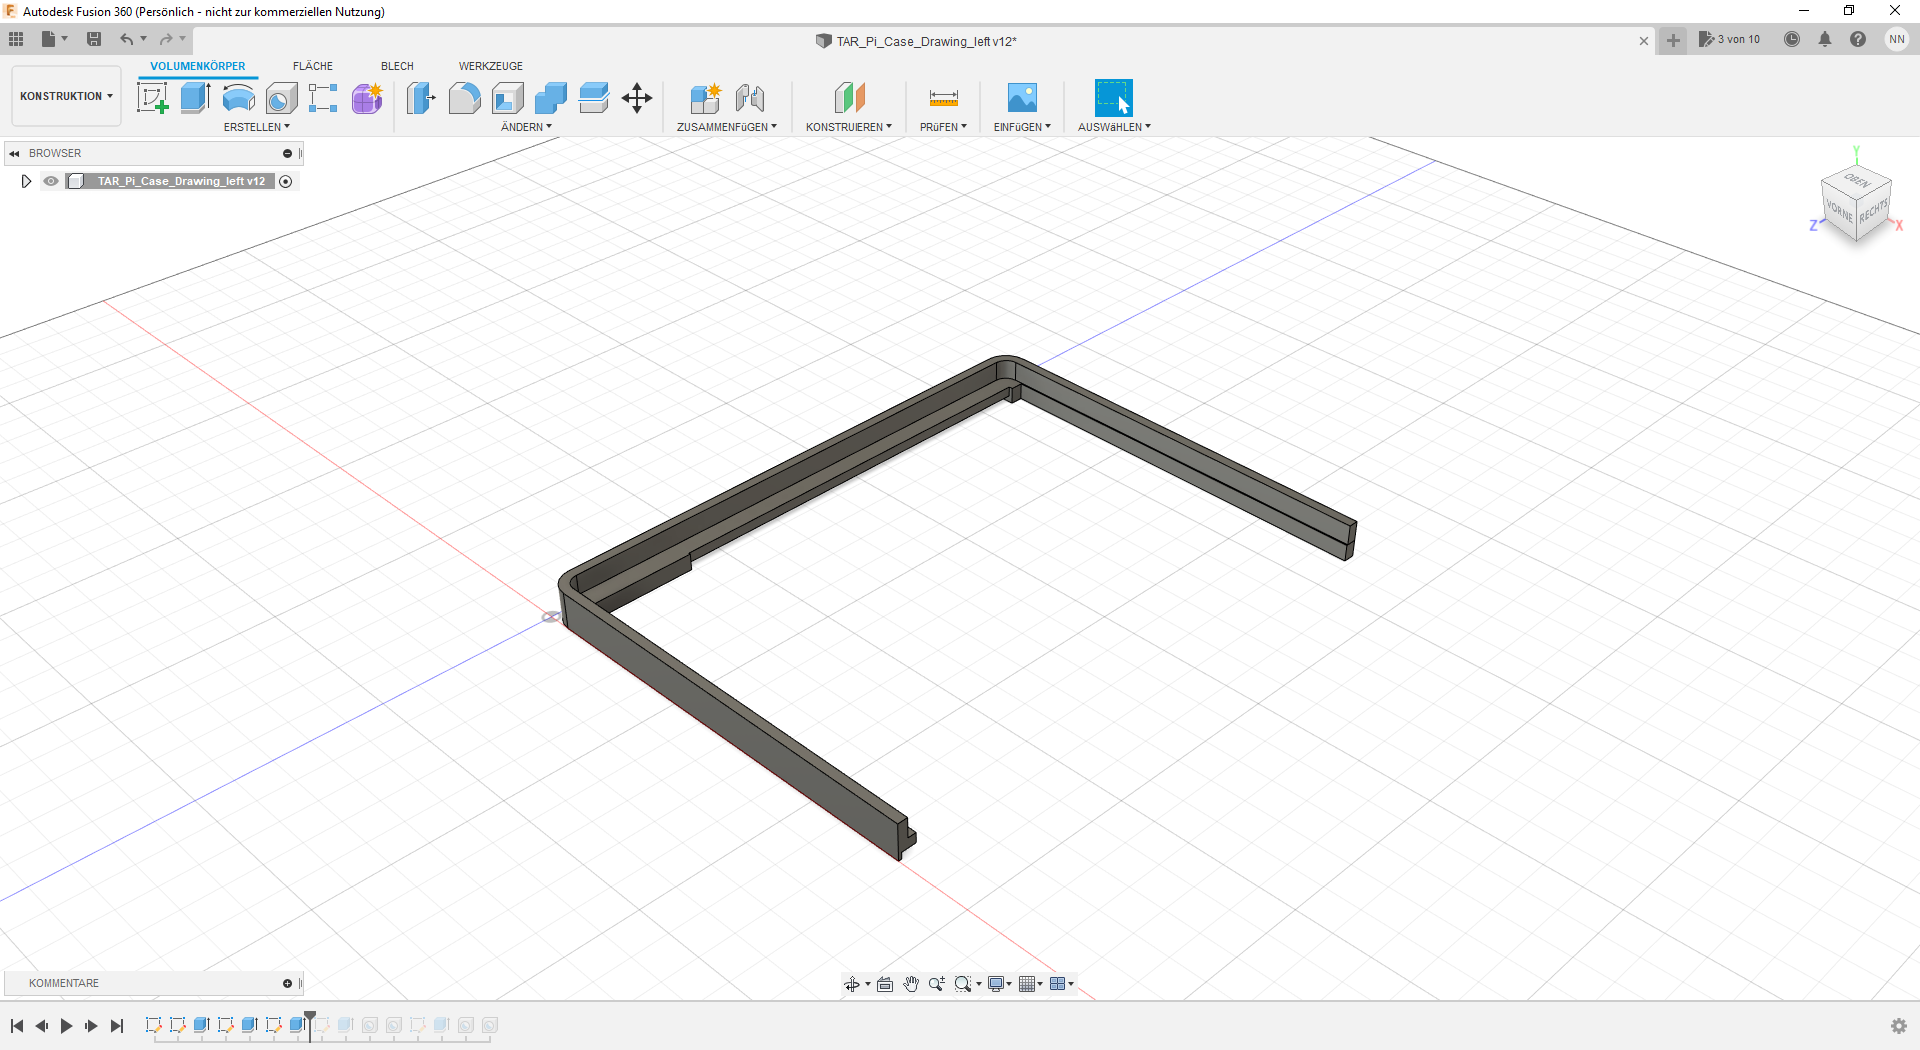
\includegraphics[width=\linewidth]{img/konstruktion_gehaeuse_links_005.png}
		\caption[Extrusion der Hauptwand]{Extrusion der Hauptwand}
		\label{fig:design-left-05}
	\end{subfigure}
	\begin{subfigure}[t]{.3\linewidth}
		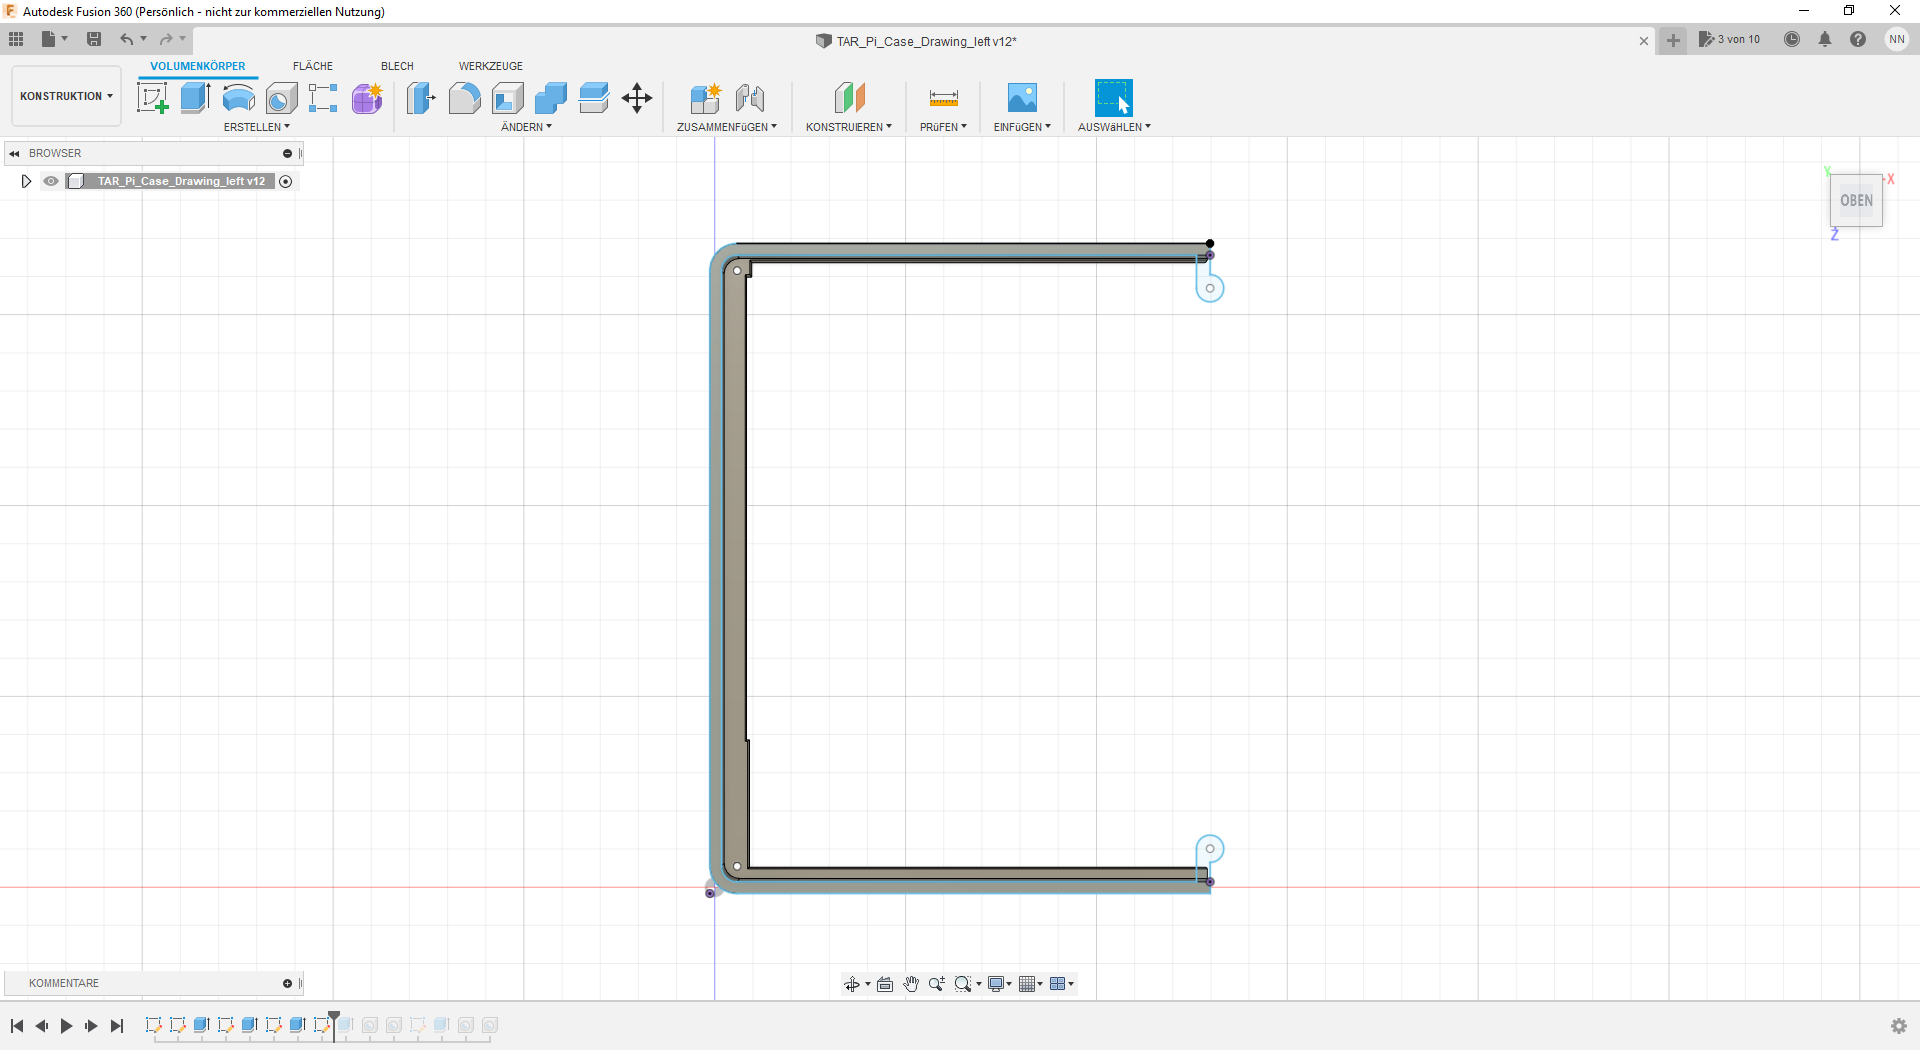
\includegraphics[width=\linewidth]{img/konstruktion_gehaeuse_links_006.png}
		\caption[Zeichnung der Verbindungsstücke]{Zeichnung der Verbindungsstücke}
		\label{fig:design-left-06}
	\end{subfigure}
	\begin{subfigure}[t]{.3\linewidth}
		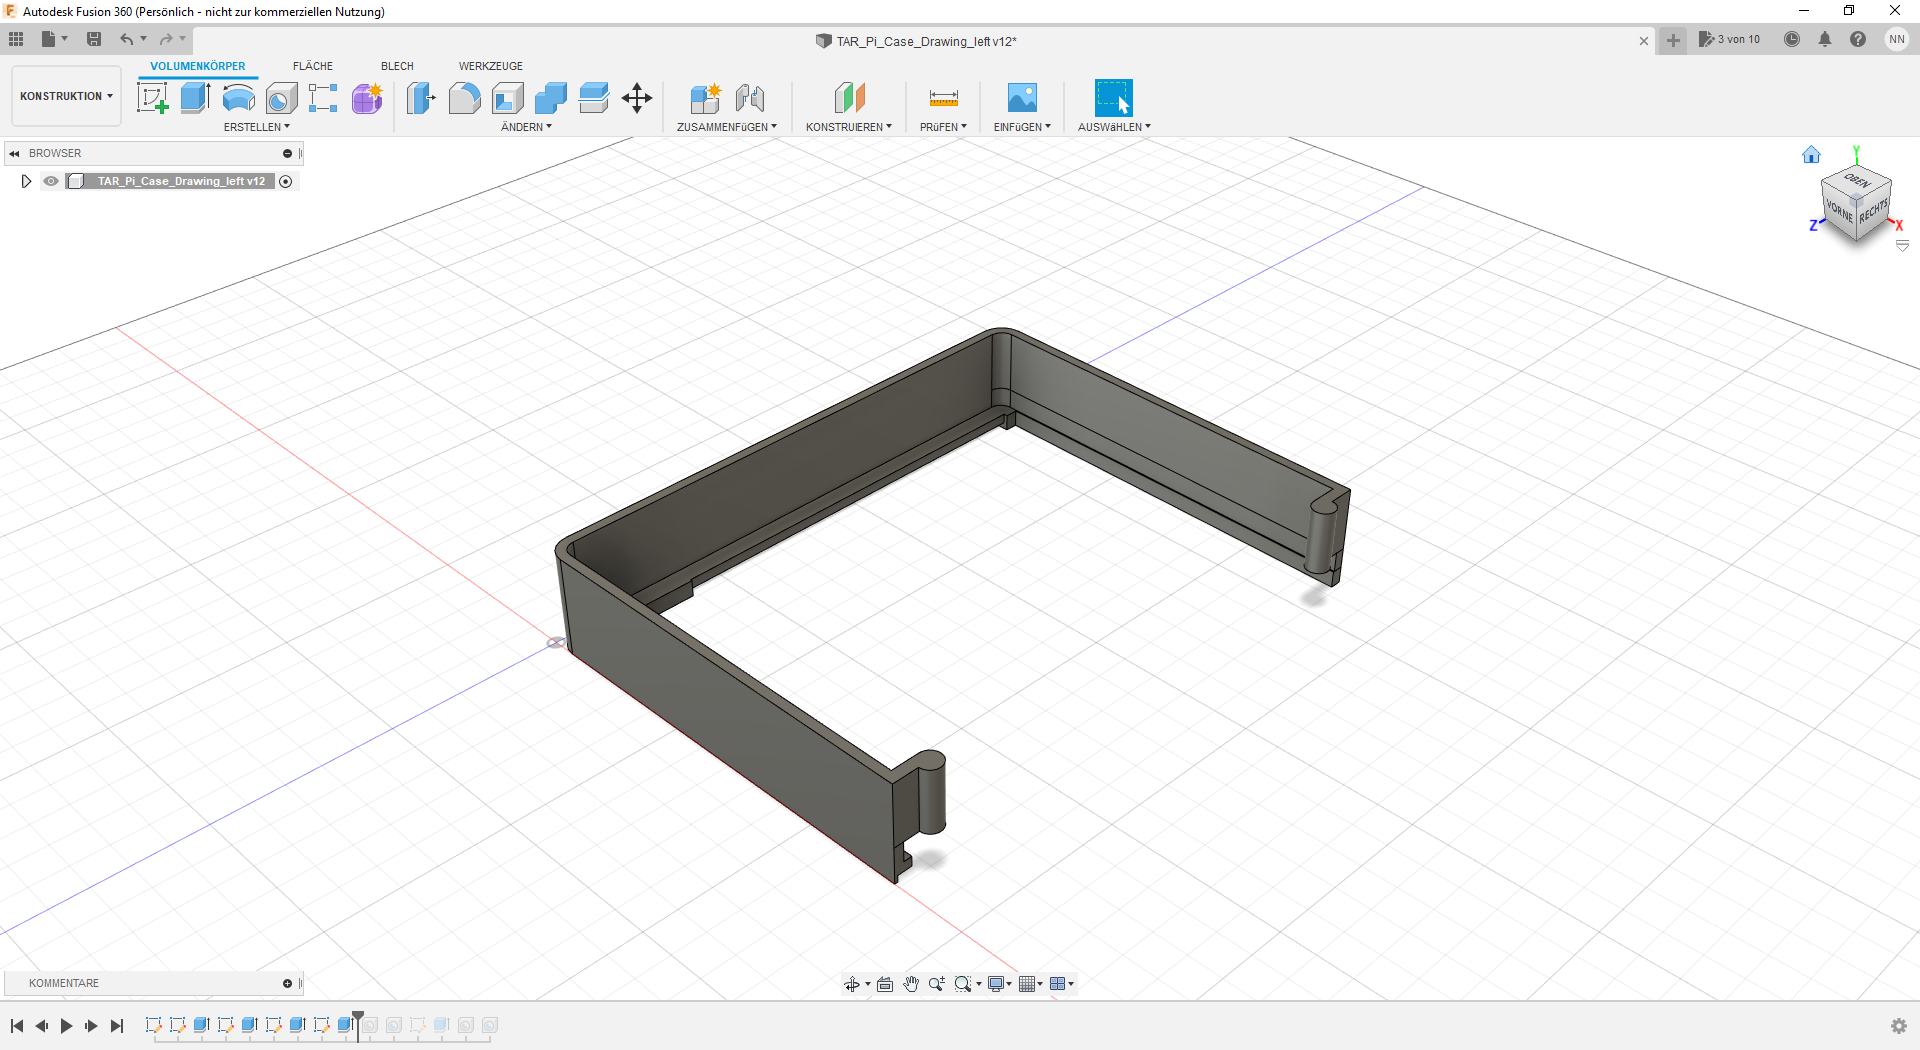
\includegraphics[width=\linewidth]{img/konstruktion_gehaeuse_links_007.png}
		\caption[Extrusion der Hauptwand mit Verbindungsstücken]{Extrusion der Hauptwand mit Verbindungsstücken}
		\label{fig:design-left-07}
	\end{subfigure}
	\begin{subfigure}[t]{.3\linewidth}
		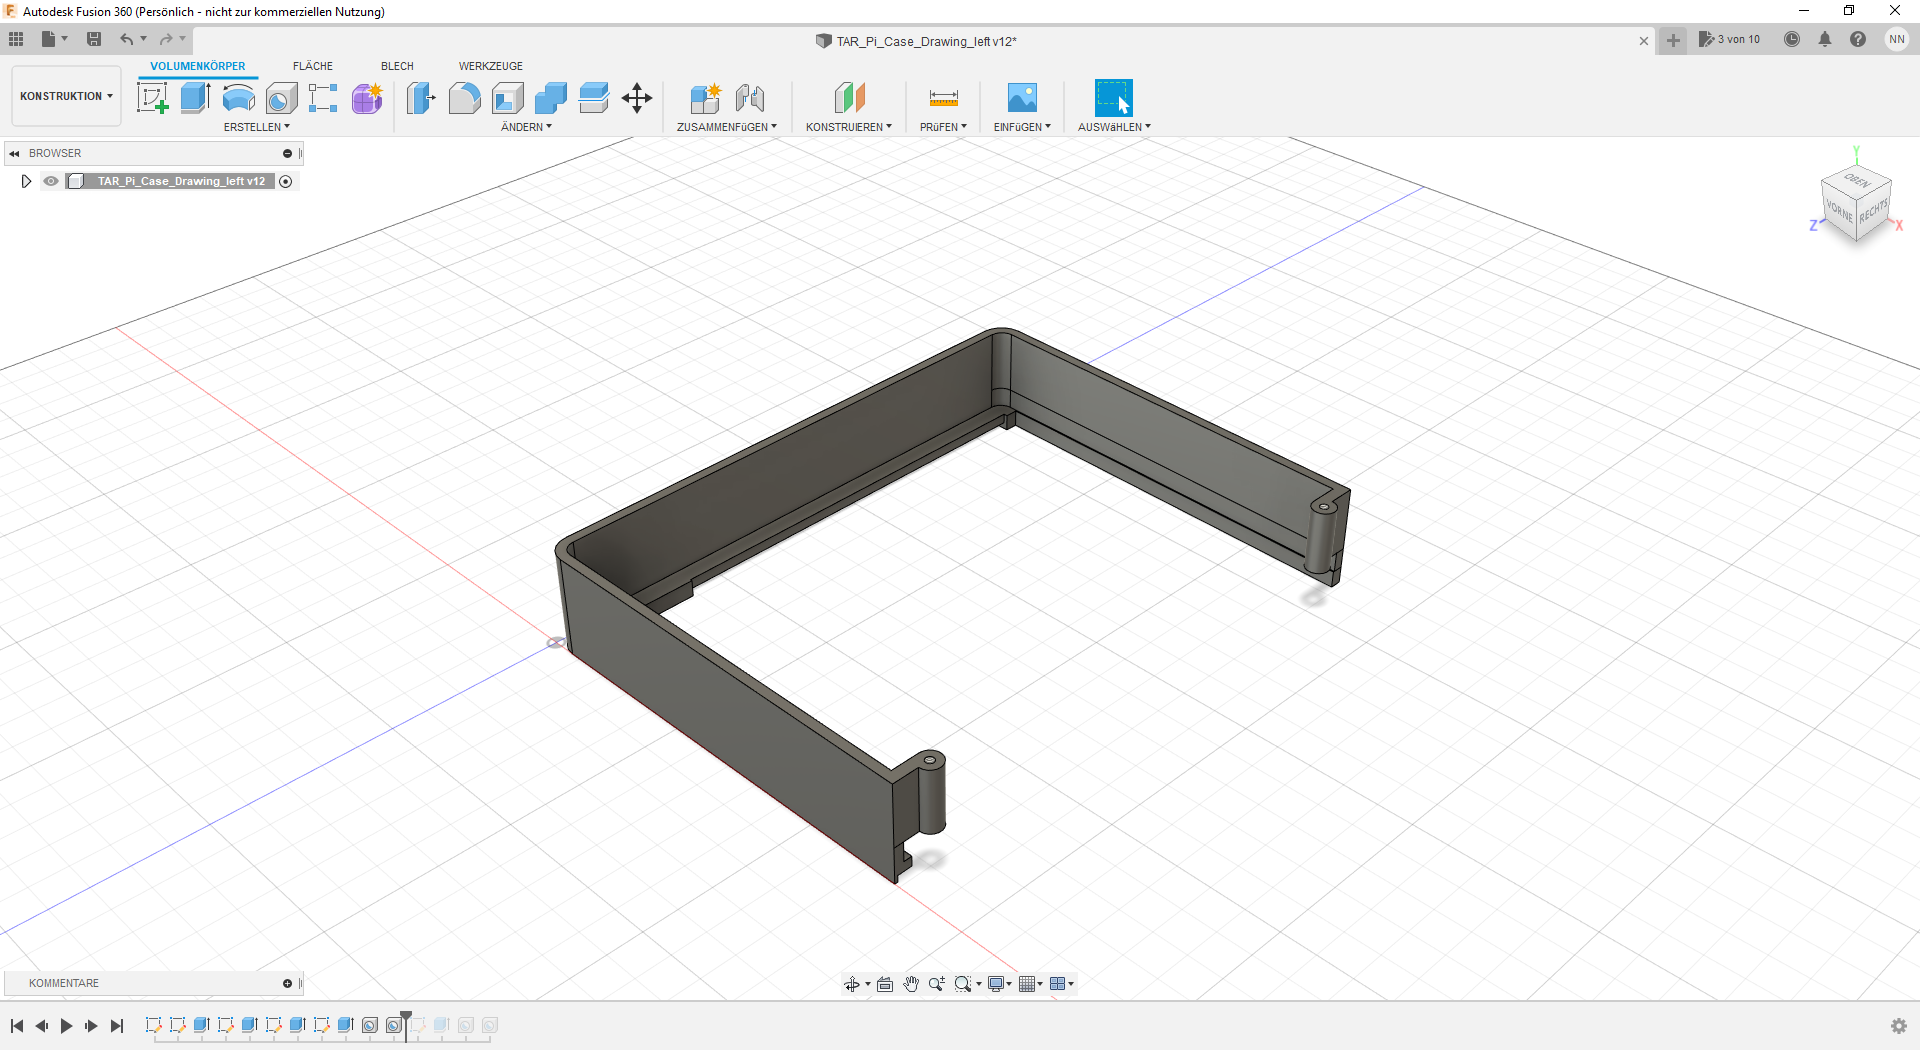
\includegraphics[width=\linewidth]{img/konstruktion_gehaeuse_links_008.png}
		\caption[Bohrung für Schrauben]{Bohrung für Schrauben}
		\label{fig:design-left-08}
	\end{subfigure}
	\begin{subfigure}[t]{.3\linewidth}
		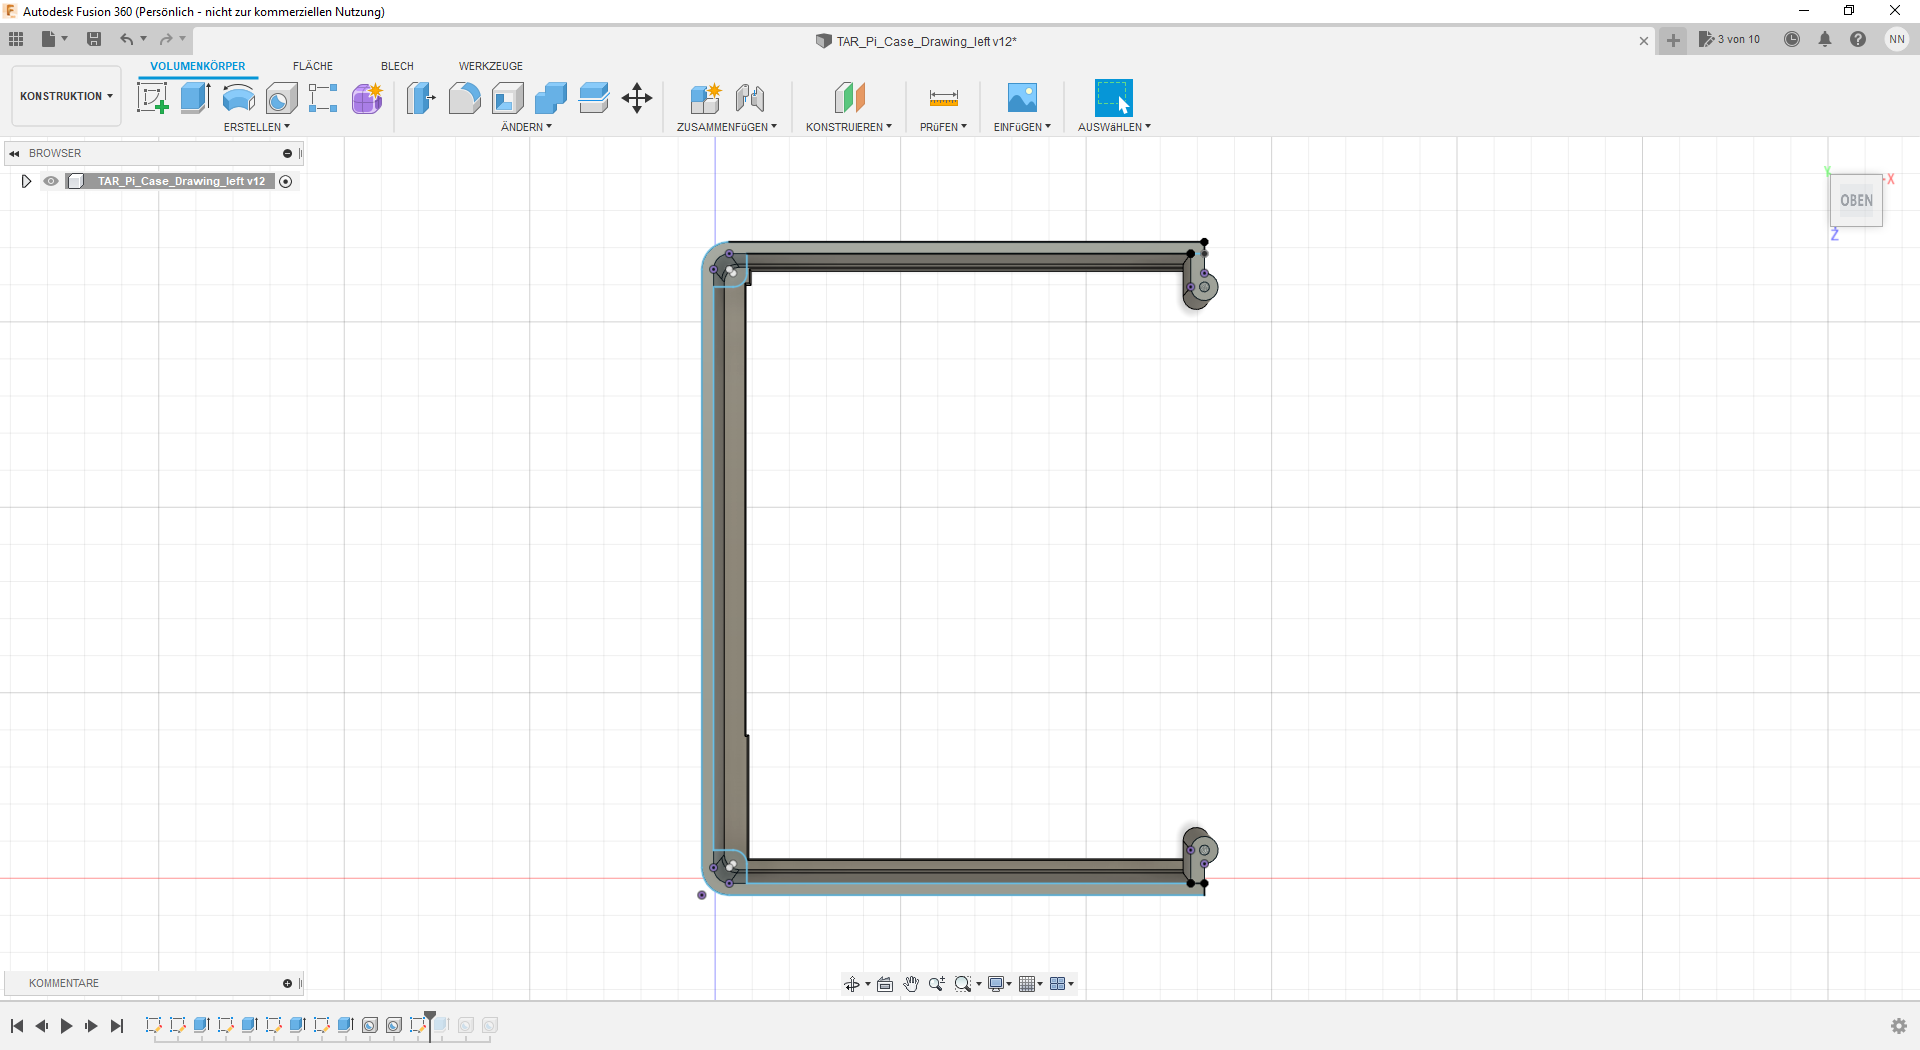
\includegraphics[width=\linewidth]{img/konstruktion_gehaeuse_links_009.png}
		\caption[Zeichnung der Deckelverbindung]{Zeichnung der Deckelverbindung}
		\label{fig:design-left-09}
	\end{subfigure}
	\begin{subfigure}[t]{.3\linewidth}
		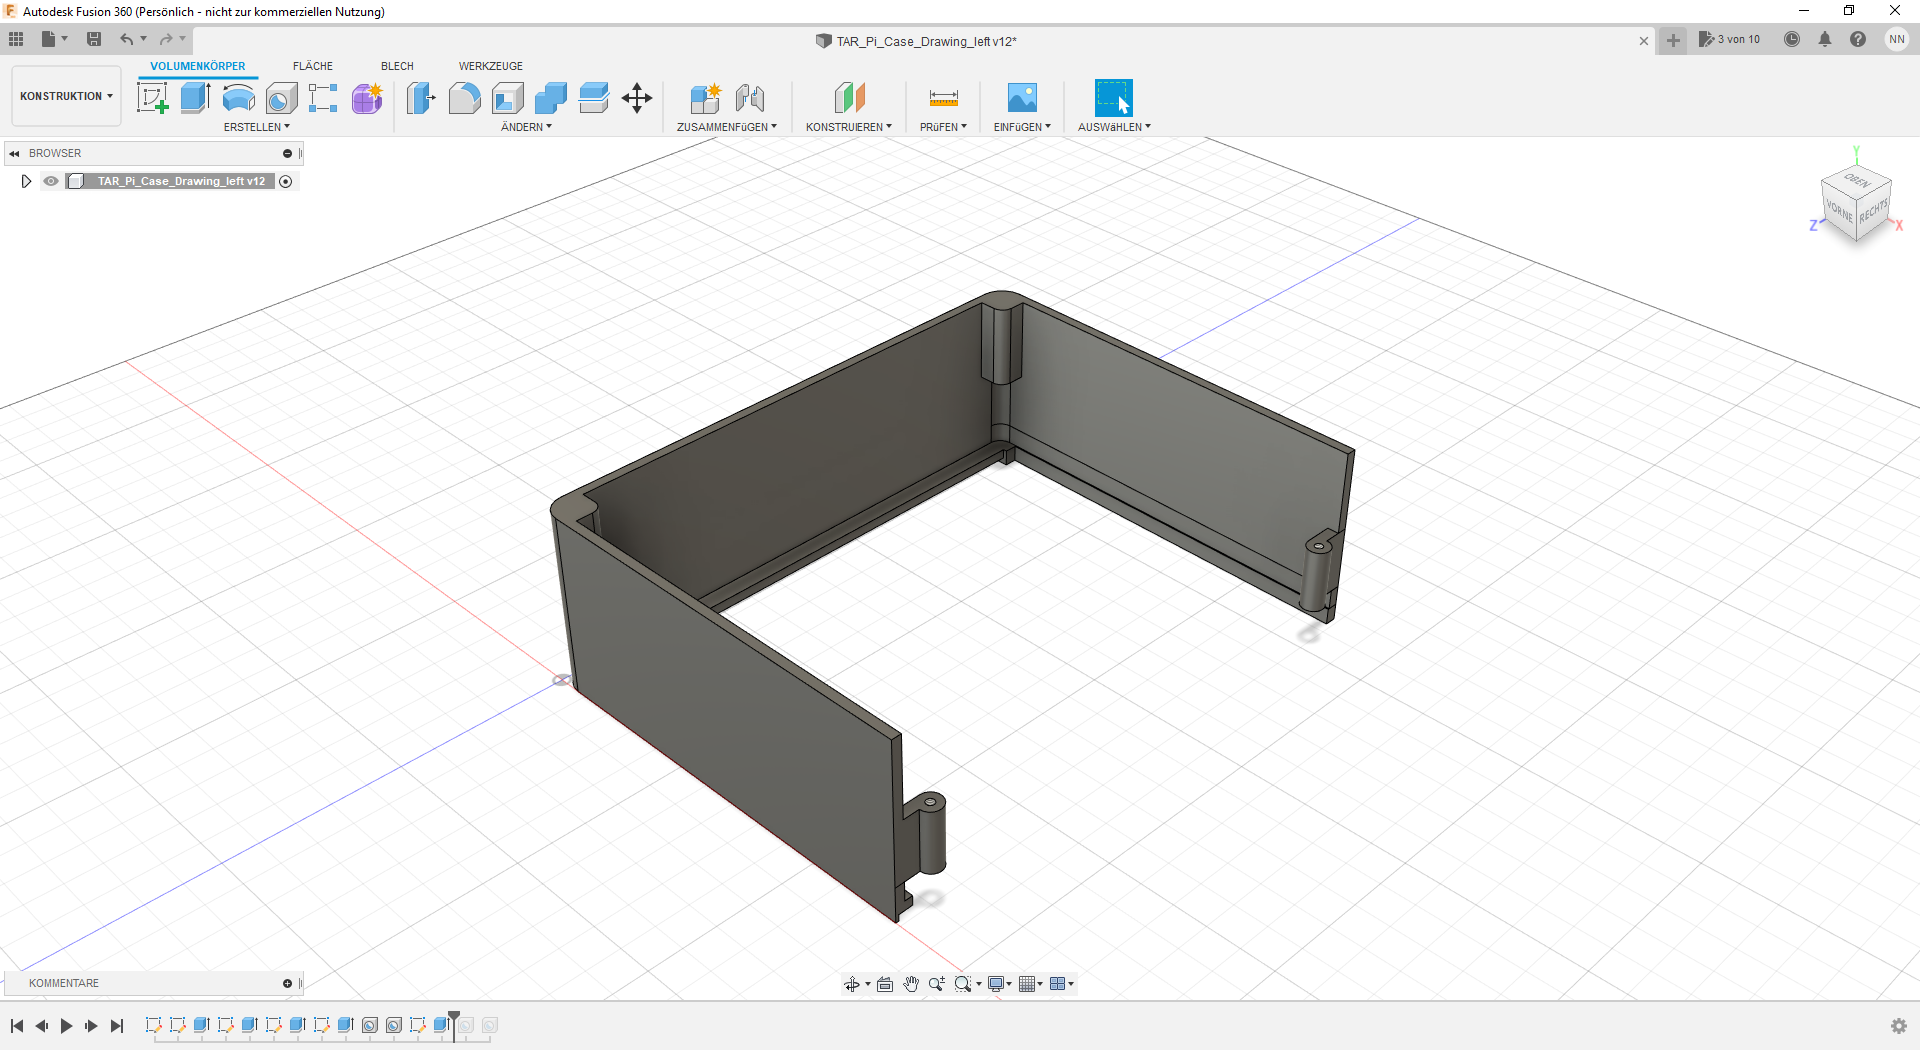
\includegraphics[width=\linewidth]{img/konstruktion_gehaeuse_links_010.png}
		\caption[Extrusion der Hauptwand mit Deckelverbindung]{Extrusion der Hauptwand mit Deckelverbindung}
		\label{fig:design-left-10}
	\end{subfigure}
	\begin{subfigure}[t]{.3\linewidth}
		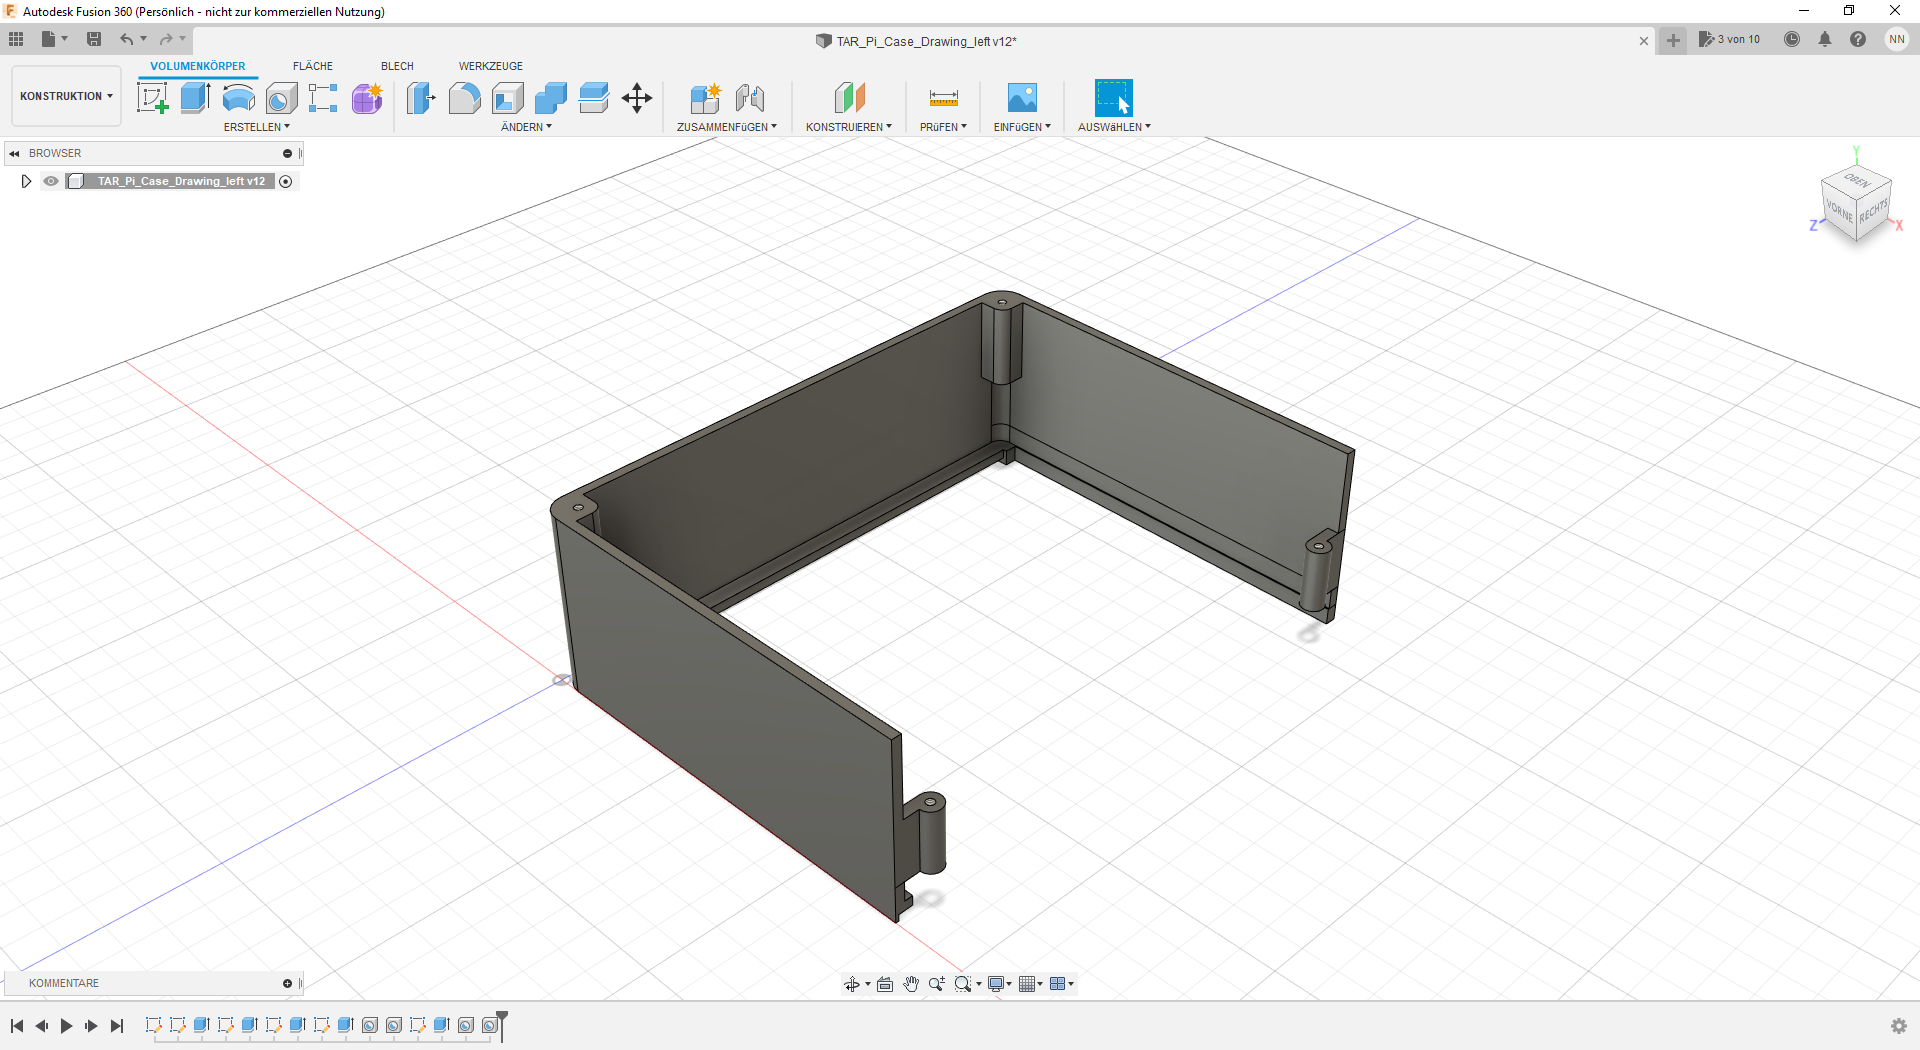
\includegraphics[width=\linewidth]{img/konstruktion_gehaeuse_links_011.png}
		\caption[Bohrungen der Deckelverbindung]{Bohrungen der Deckelverbindung}
		\label{fig:design-left-11}
	\end{subfigure}
	\caption[Entwurf des linken Wandteils]{Entwurf des linken Wandteils}
	\label{fig:design-left}
\end{figure}\par
\newpage
\paragraph{Rechtes Wandteil}
Beim rechten Teil des Gehäuses ist die Vorgehensweise weitestgehend die selbe wie beim linken Gehäuseteil (vgl. Abb. \ref{fig:design-right-01}: \nameref{fig:design-right-01} - Abb. \ref{fig:design-right-08}: \nameref{fig:design-right-08} mit Abb. \ref{fig:design-left}: \nameref{fig:design-left}). 
Der Unterschied zwischen beiden Teilen, abgesehen von den Verbindungsstücken und der Aussparung für das Flachkabel des Bildschirms, sind zusätzlich die Aussparungen für Lüfter, Antenne, Netzwerkanschluss und Strombuchse. \\
\noindent Für den Lüfter und die Antenne haben wir auf dem oberen Teil des Gehäuses eine Zeichnung aufgelegt (vgl. Abb. \ref{fig:design-right-09}: \nameref{fig:design-right-09}), die  wir dann ins Negative extrudiert haben, um die gezeichnete Fläche aus dem Gehäuse zu löschen (vgl. Abb. \ref{fig:design-right-10}: \nameref{fig:design-right-10}). 
Mit der selben Vorgehensweise haben wir die Aussparung für eine RJ45-Verlängerung und eine 5,5 mm DC-Buchse gesetzt. 
Zuerst haben wir die Zeichnung für die Aussparung auf die Seite gelegt (vgl. Abb.  \ref{fig:design-right-11}: \nameref{fig:design-right-11}) und diese dann ebenfalls ins Negative extrudiert (vgl. Abb. \ref{fig:design-right-12}: \nameref{fig:design-right-12}). \\
\noindent Um für die Befestigung der 5,5 mm DC-Buchse eine Unterlage im Gehäuse zu haben, haben wir der Grundriss eines Rechtecks auf die Innenseite des Gehäusebodens gelegt (vgl. Abb.  \ref{fig:design-right-13}: \nameref{fig:design-right-13}) und extrudiert (vgl. Abb. \ref{fig:design-right-14}: \nameref{fig:design-right-14}), um die Möglichkeit zu haben, die Buchse mit dem Gehäuse zu verkleben. 
Damit die Buchse nicht zu tief im Gehäuse steckt, haben wir eine Zeichnung eines konzentrischen Kreises auf die bereits vorhandene Aussparung auf die Innenseite gelegt  (vgl. Abb.  \ref{fig:design-right-15}: \nameref{fig:design-right-15}) und dann um einige Millimeter ins Negative verkürzt, um die Aussparung zu generieren (vgl. Abb. \ref{fig:design-right}: \nameref{fig:design-right}).\par
\begin{figure}[H]
	\begin{subfigure}[t]{.3\linewidth}
		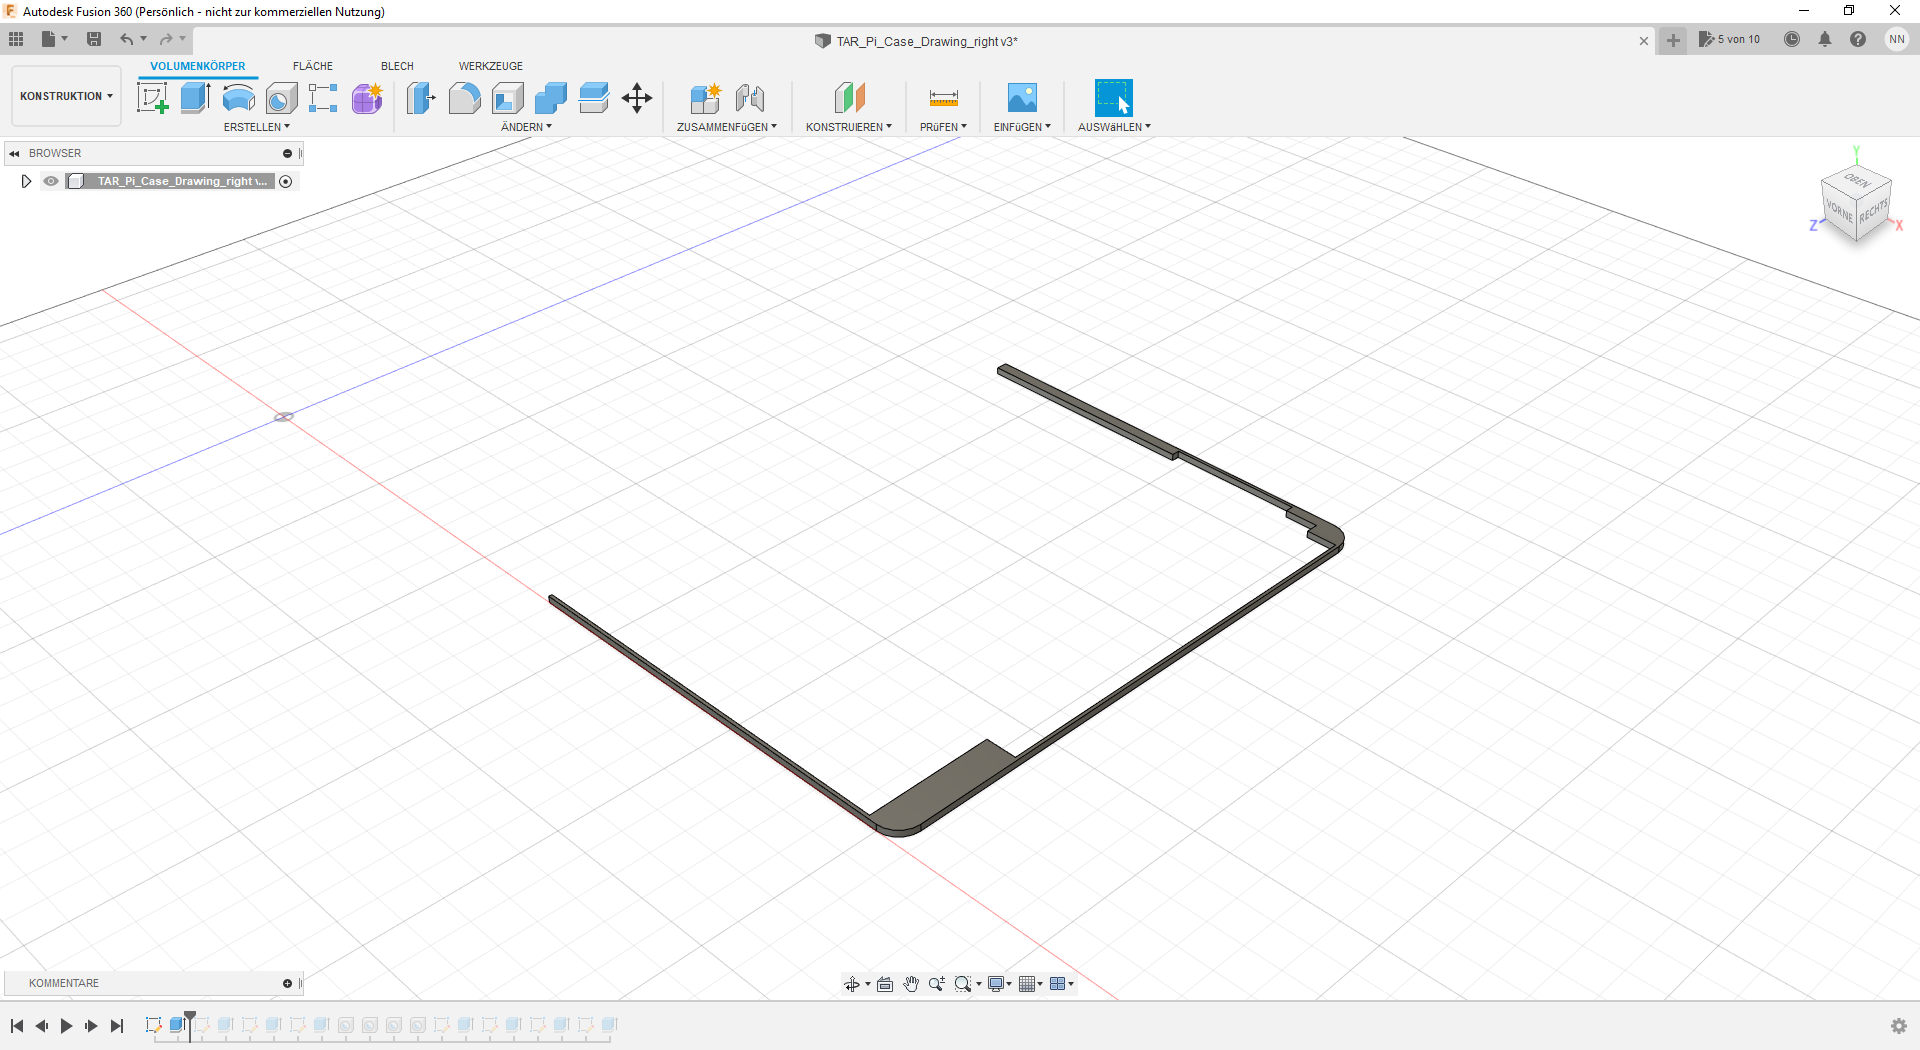
\includegraphics[width=\linewidth]{img/konstruktion_gehaeuse_rechts_001.png}
		\caption[Extrusion der Grundzeichnung]{Extrusion der Grundzeichnung}
		\label{fig:design-right-01}
	\end{subfigure}
	\begin{subfigure}[t]{.3\linewidth}
		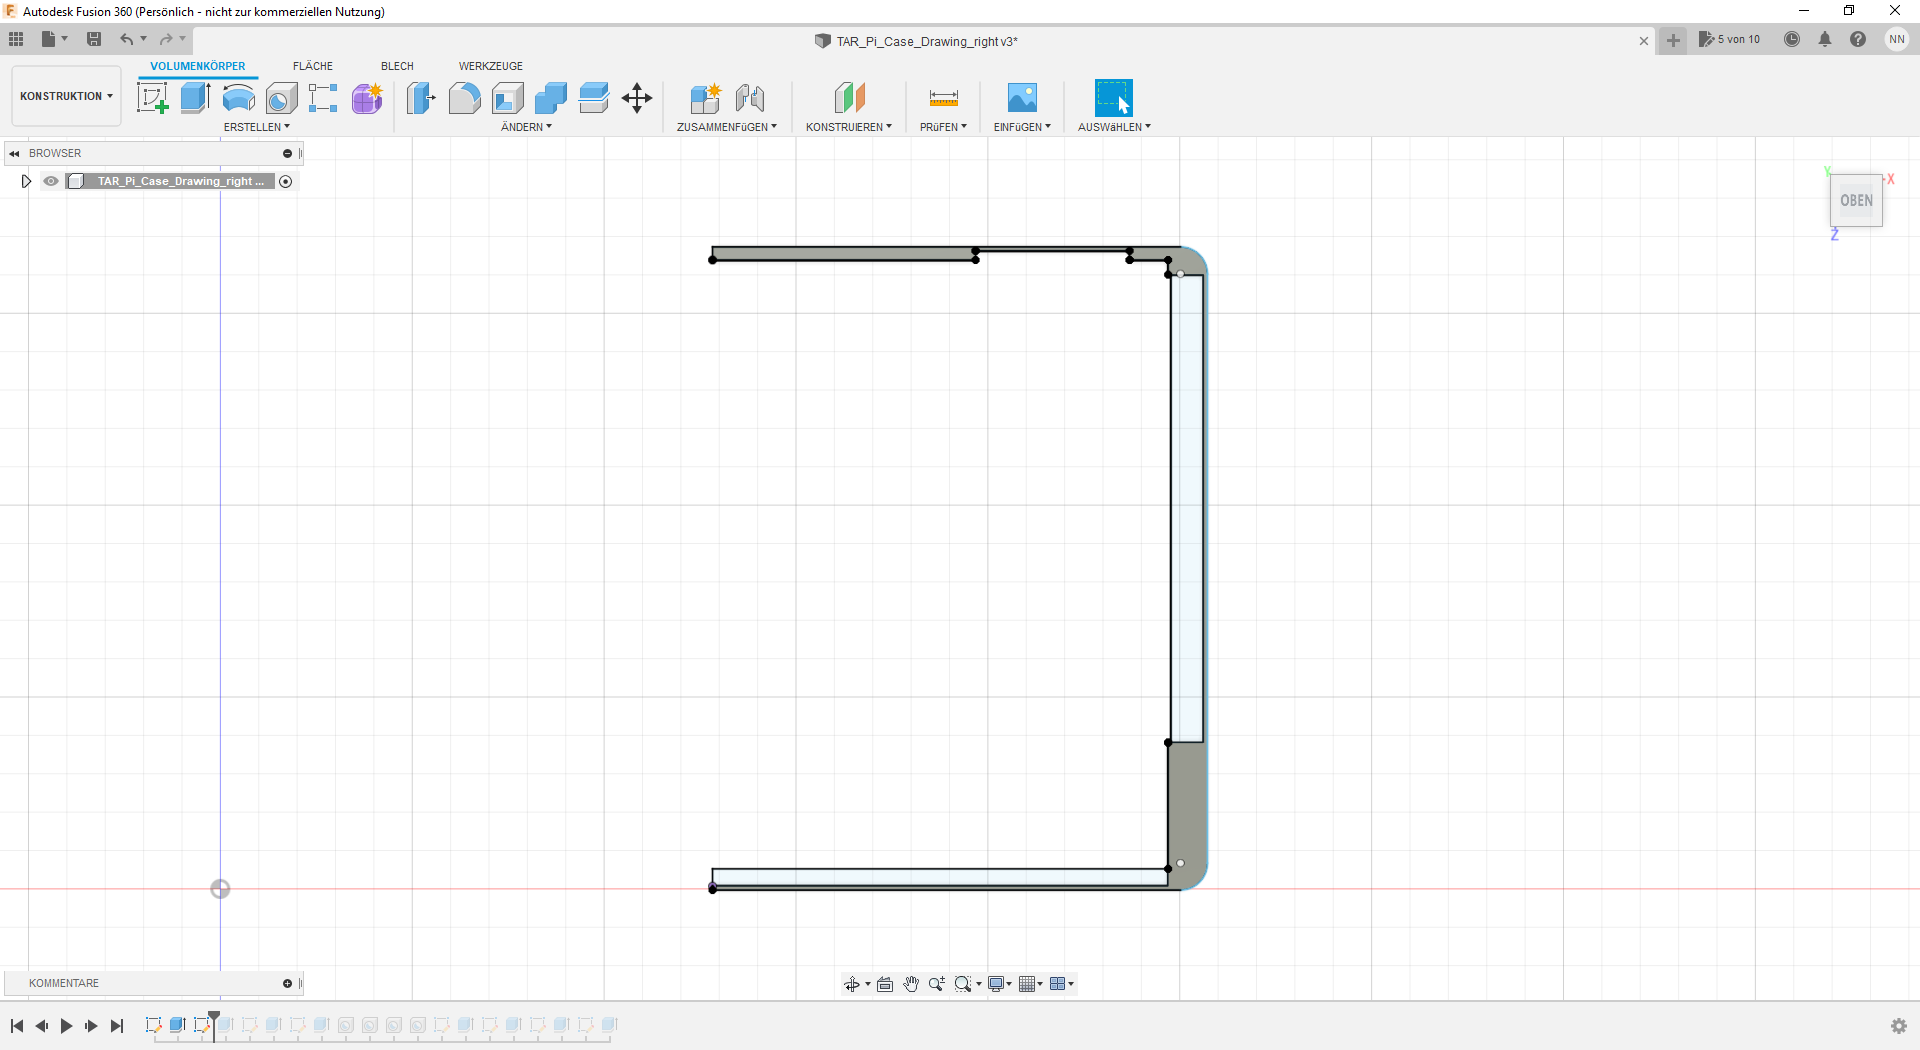
\includegraphics[width=\linewidth]{img/konstruktion_gehaeuse_rechts_002.png}
		\caption[Erstellung der Folgezeichnung um Blech]{Erstellung der Folgezeichnung um Blech}
		\label{fig:design-right-02}
	\end{subfigure}
	\begin{subfigure}[t]{.3\linewidth}
		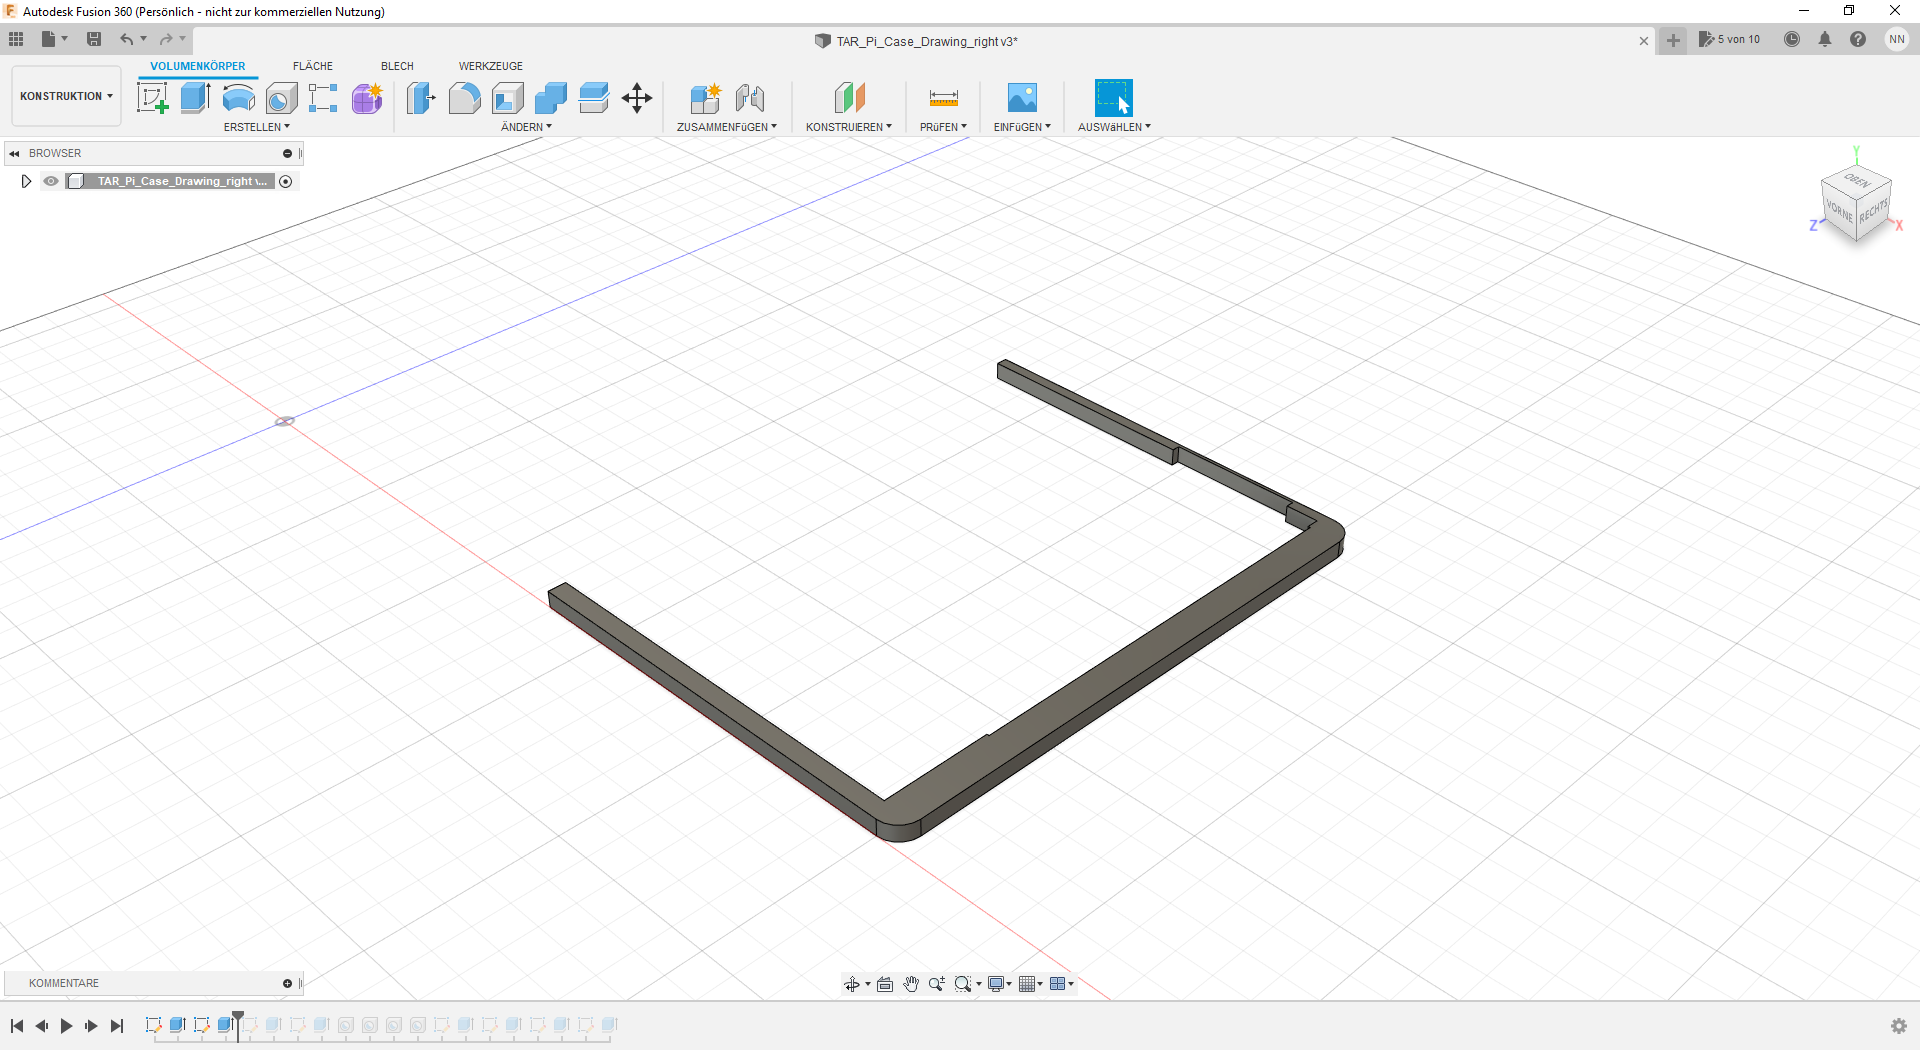
\includegraphics[width=\linewidth]{img/konstruktion_gehaeuse_rechts_003.png}
		\caption[Extrusion der neuen Zeichnung]{Extrusion der neuen Zeichnung}
		\label{fig:design-right-03}
	\end{subfigure}
	\begin{subfigure}[t]{.3\linewidth}
		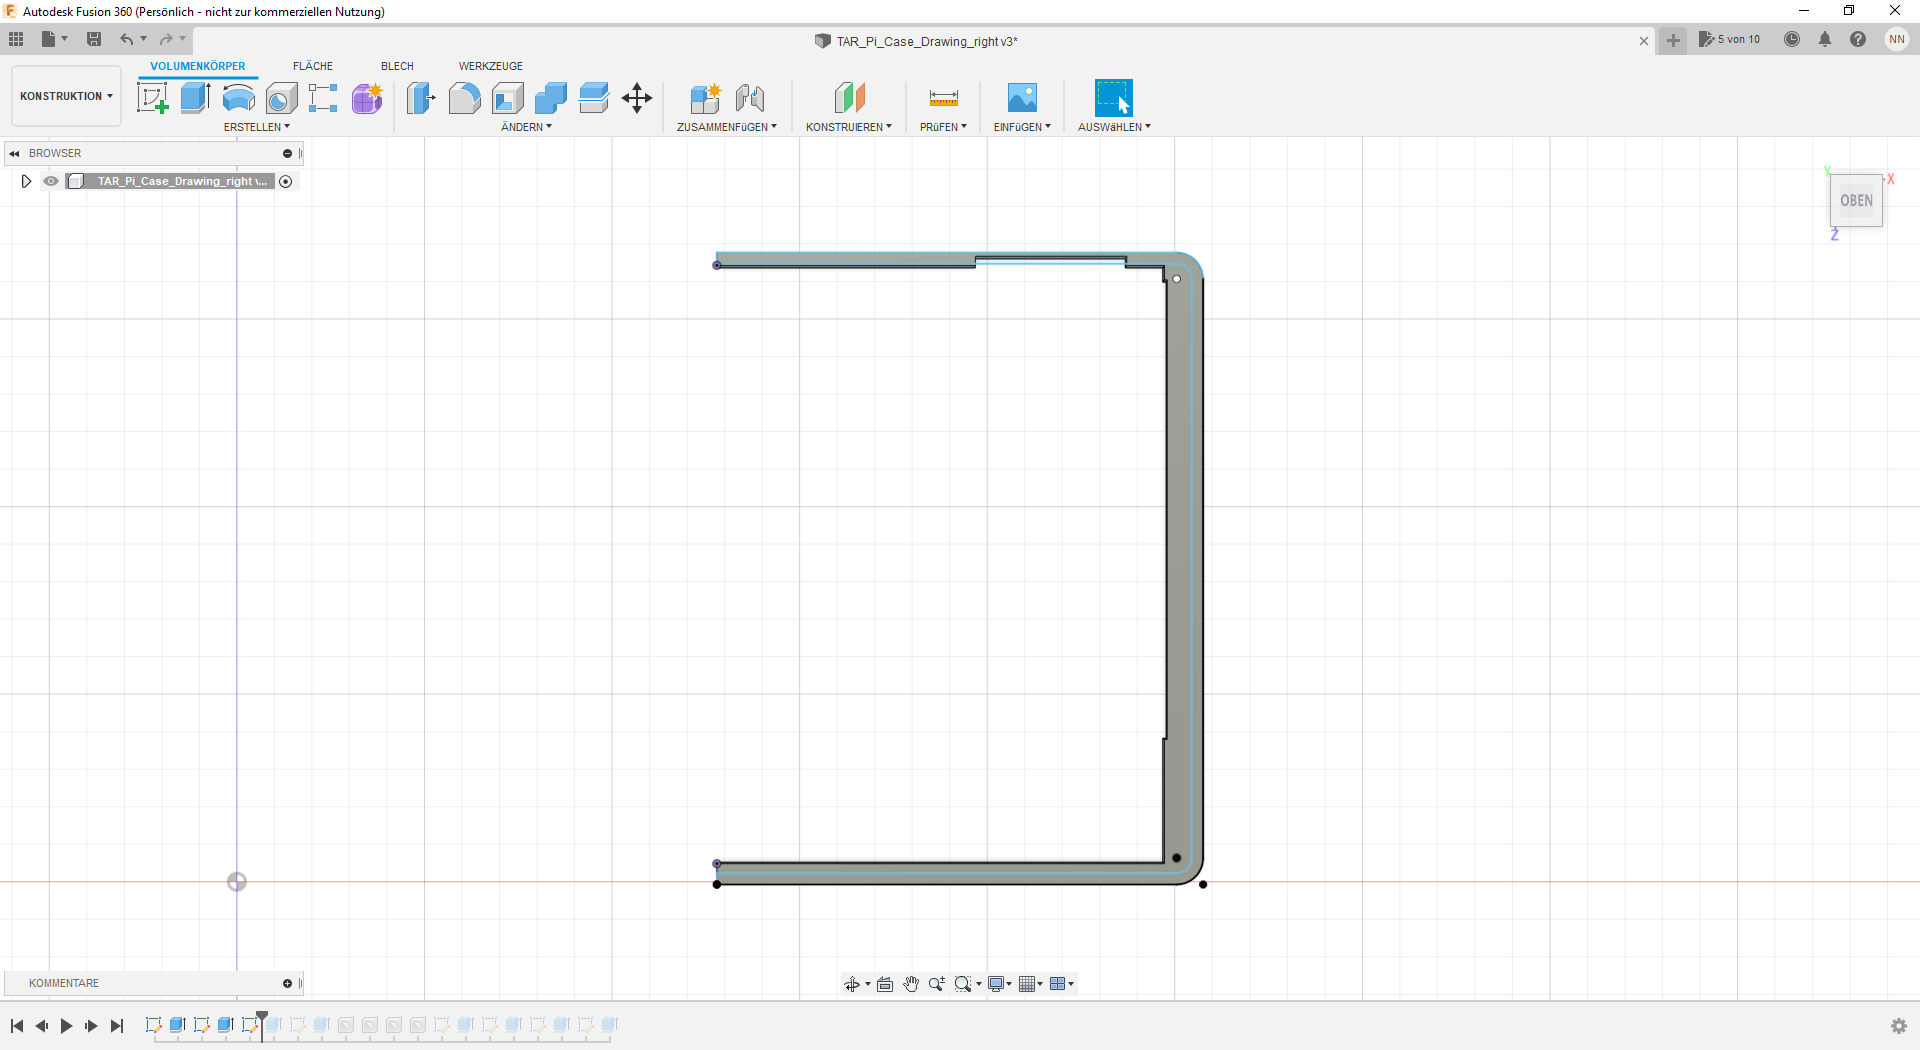
\includegraphics[width=\linewidth]{img/konstruktion_gehaeuse_rechts_004.png}
		\caption[Zeichnung der Hauptwandstärke]{Zeichnung der Hauptwandstärke}
		\label{fig:design-right-04}
	\end{subfigure}
	\begin{subfigure}[t]{.3\linewidth}
		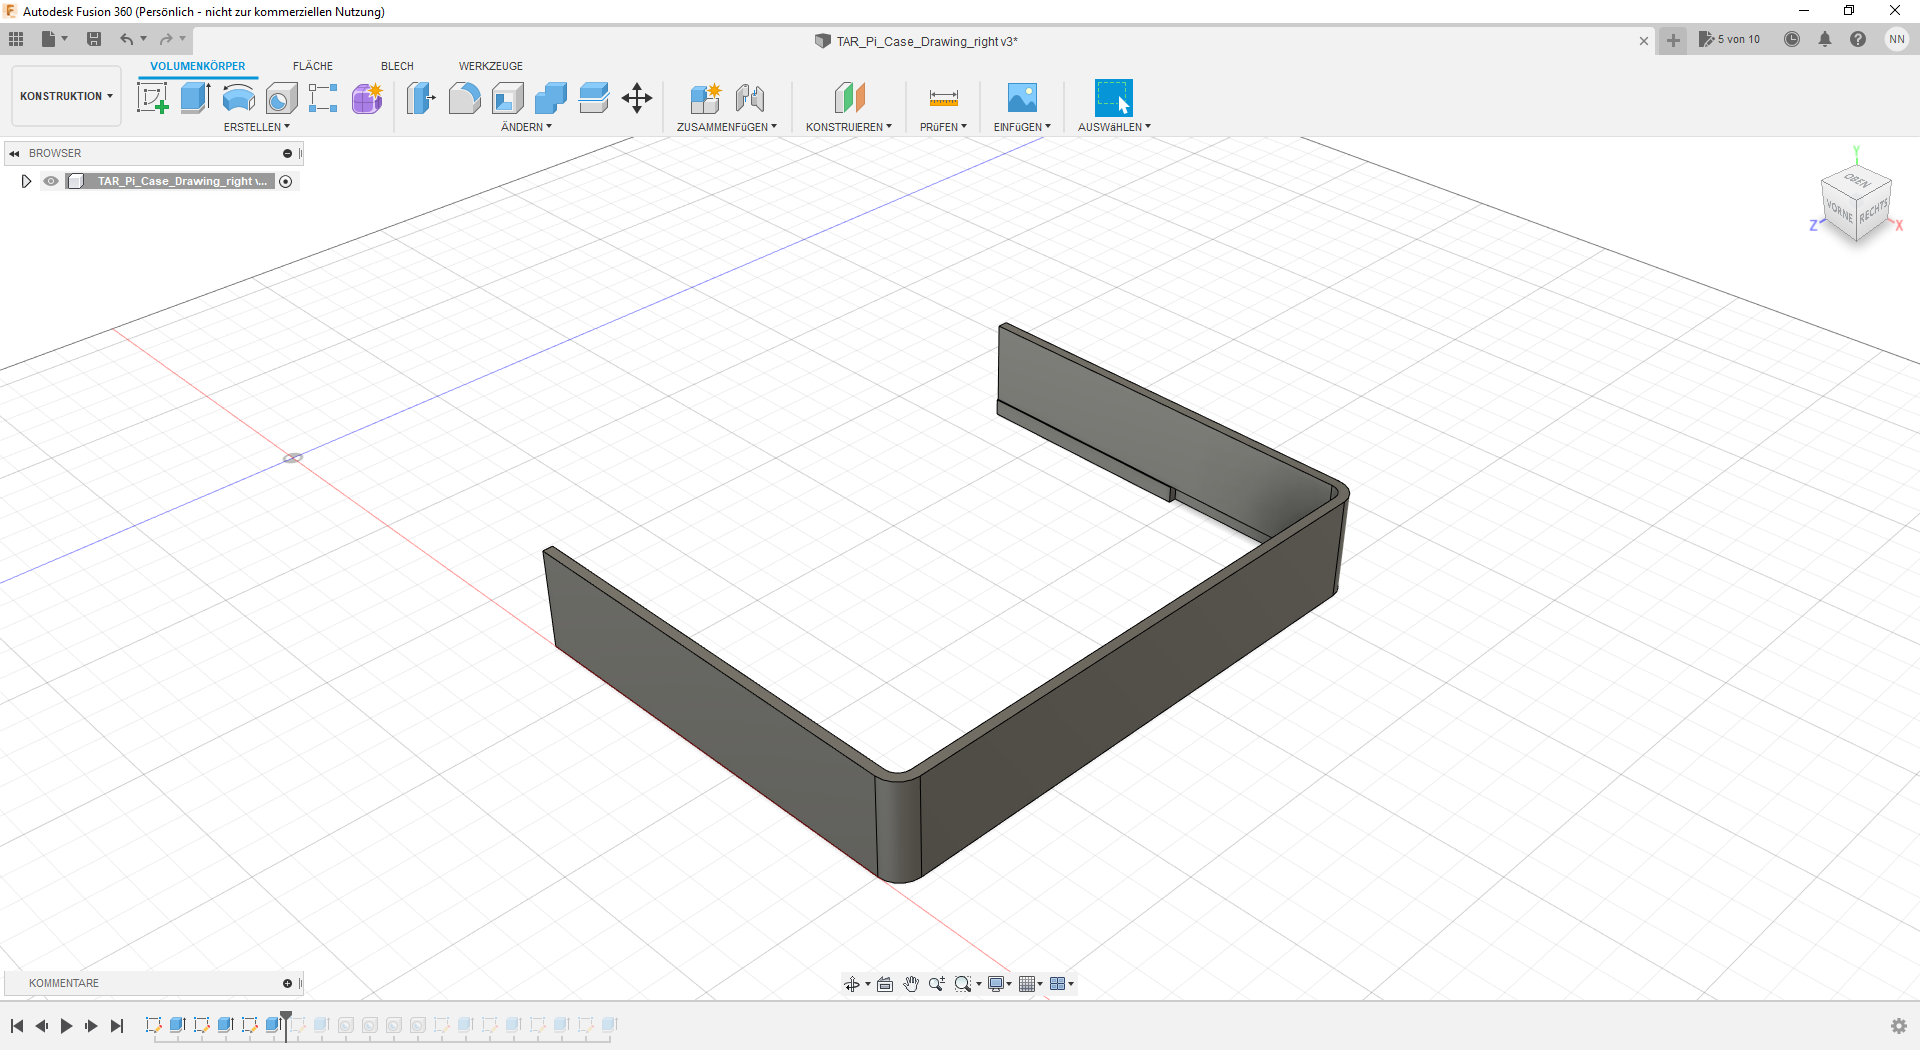
\includegraphics[width=\linewidth]{img/konstruktion_gehaeuse_rechts_005.png}
		\caption[Extrusion der Hauptwand]{Extrusion der Hauptwand}
		\label{fig:design-right-05}
	\end{subfigure}
	\begin{subfigure}[t]{.3\linewidth}
		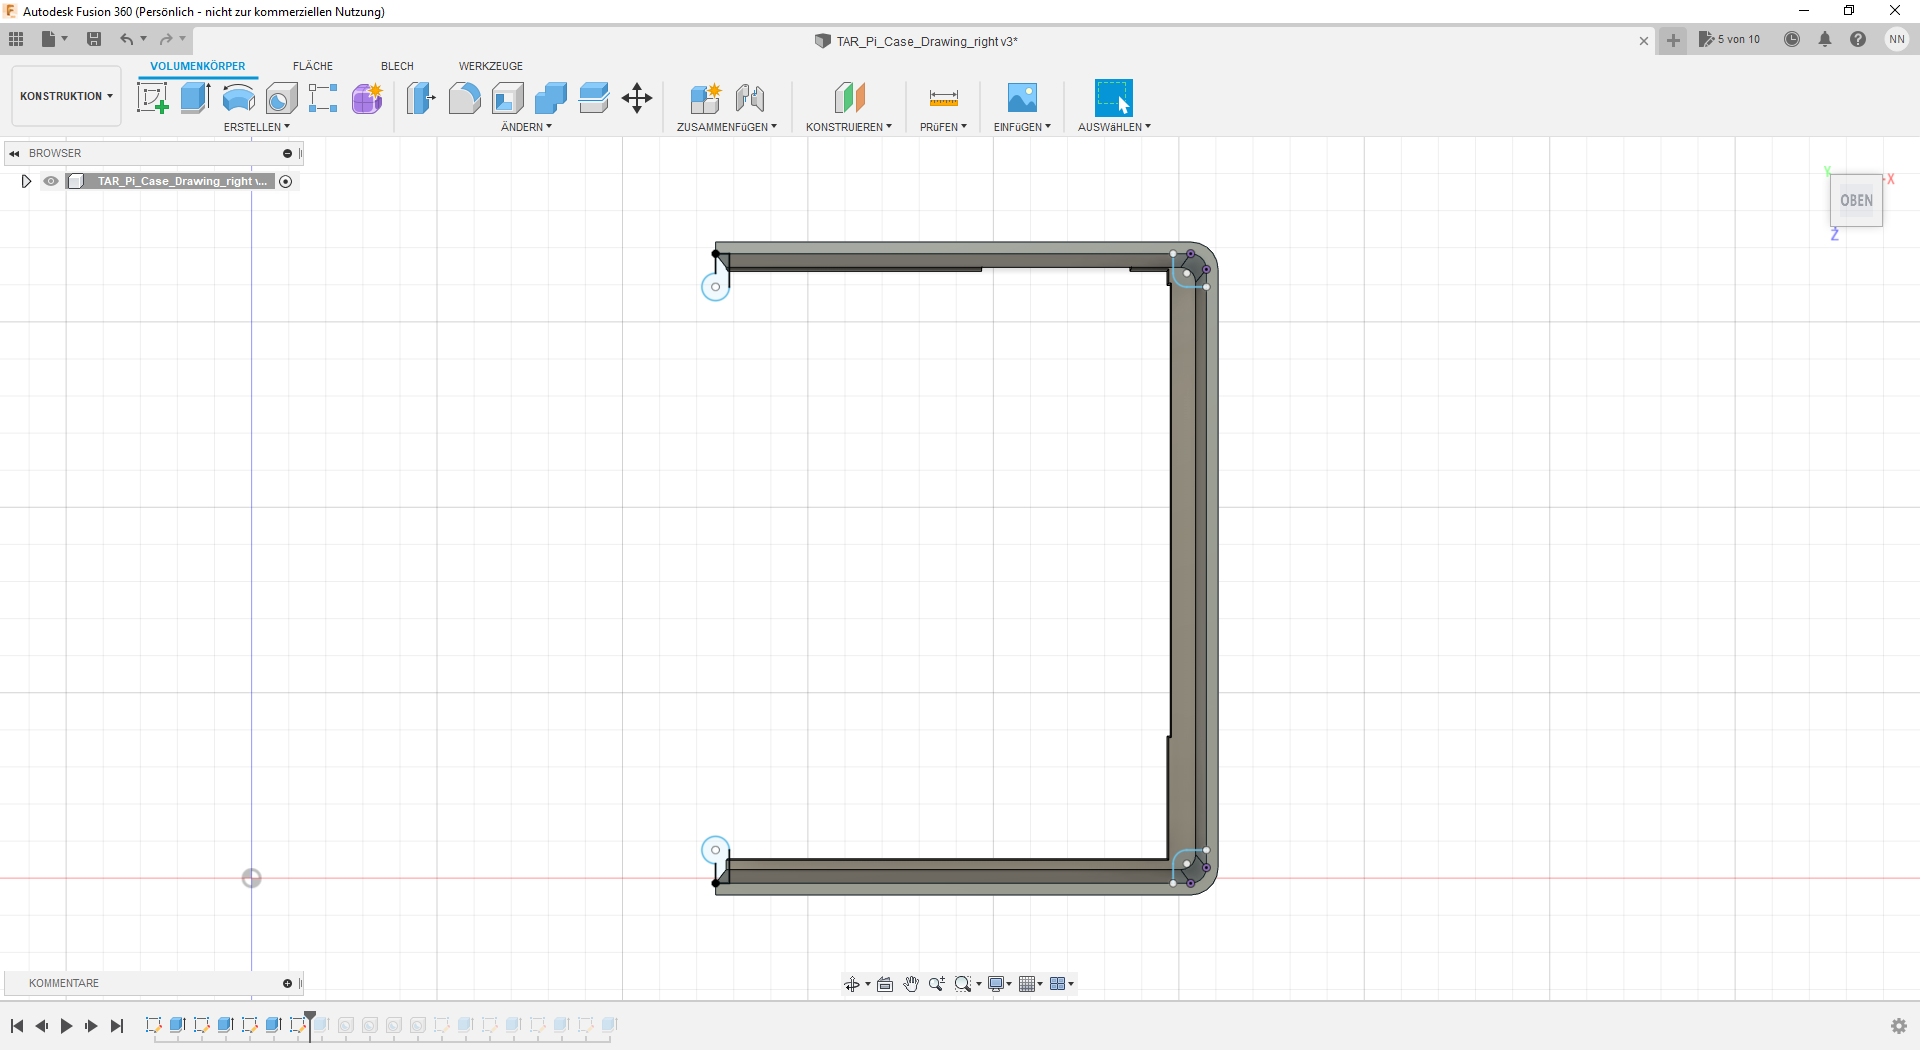
\includegraphics[width=\linewidth]{img/konstruktion_gehaeuse_rechts_006.png}
		\caption[Zeichnung der Verbindungsstücke \& Deckelverbindung]{Zeichnung der Verbindungsstücke \& Deckelverbindung}
		\label{fig:design-right-06}
	\end{subfigure}
	\begin{subfigure}[t]{.3\linewidth}
		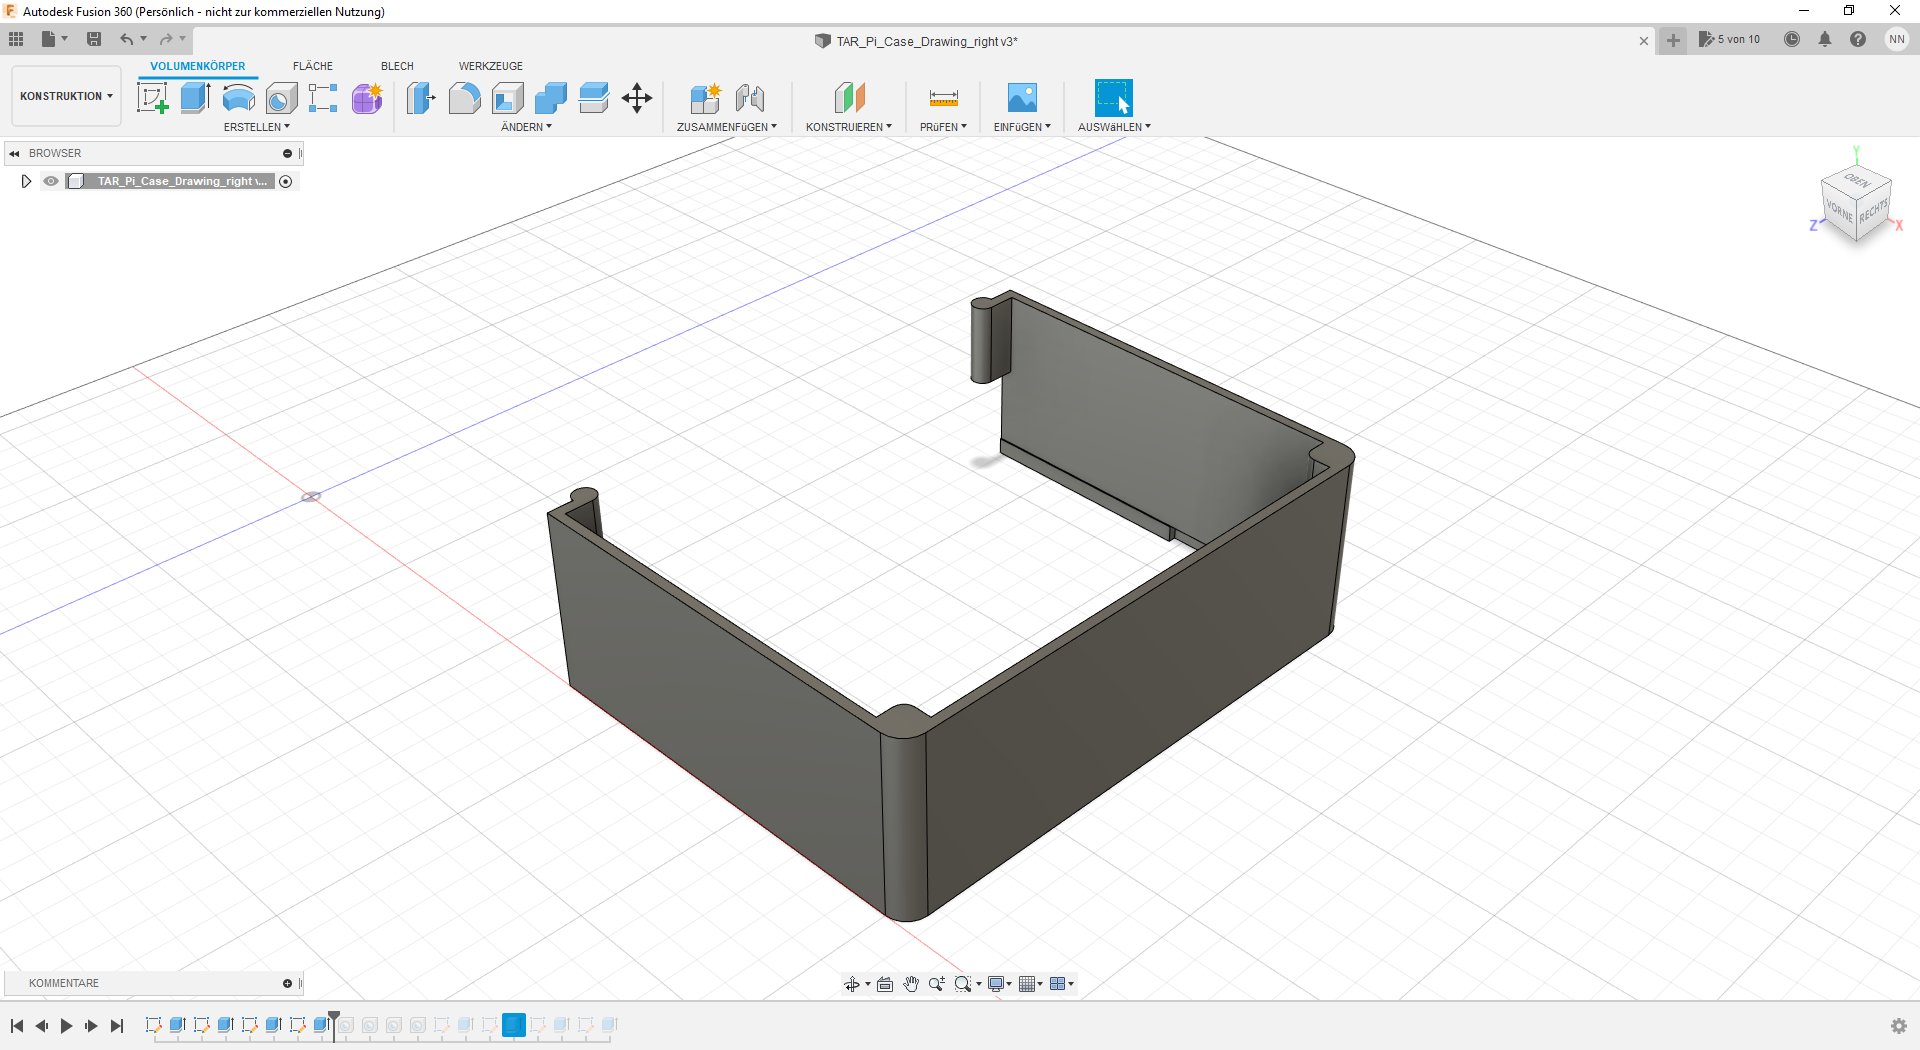
\includegraphics[width=\linewidth]{img/konstruktion_gehaeuse_rechts_007.png}
		\caption[Extrusion der Hauptwand mit Deckelverbindung]{Extrusion der Hauptwand mit Deckelverbindung}
		\label{fig:design-right-07}
	\end{subfigure}
	\begin{subfigure}[t]{.3\linewidth}
		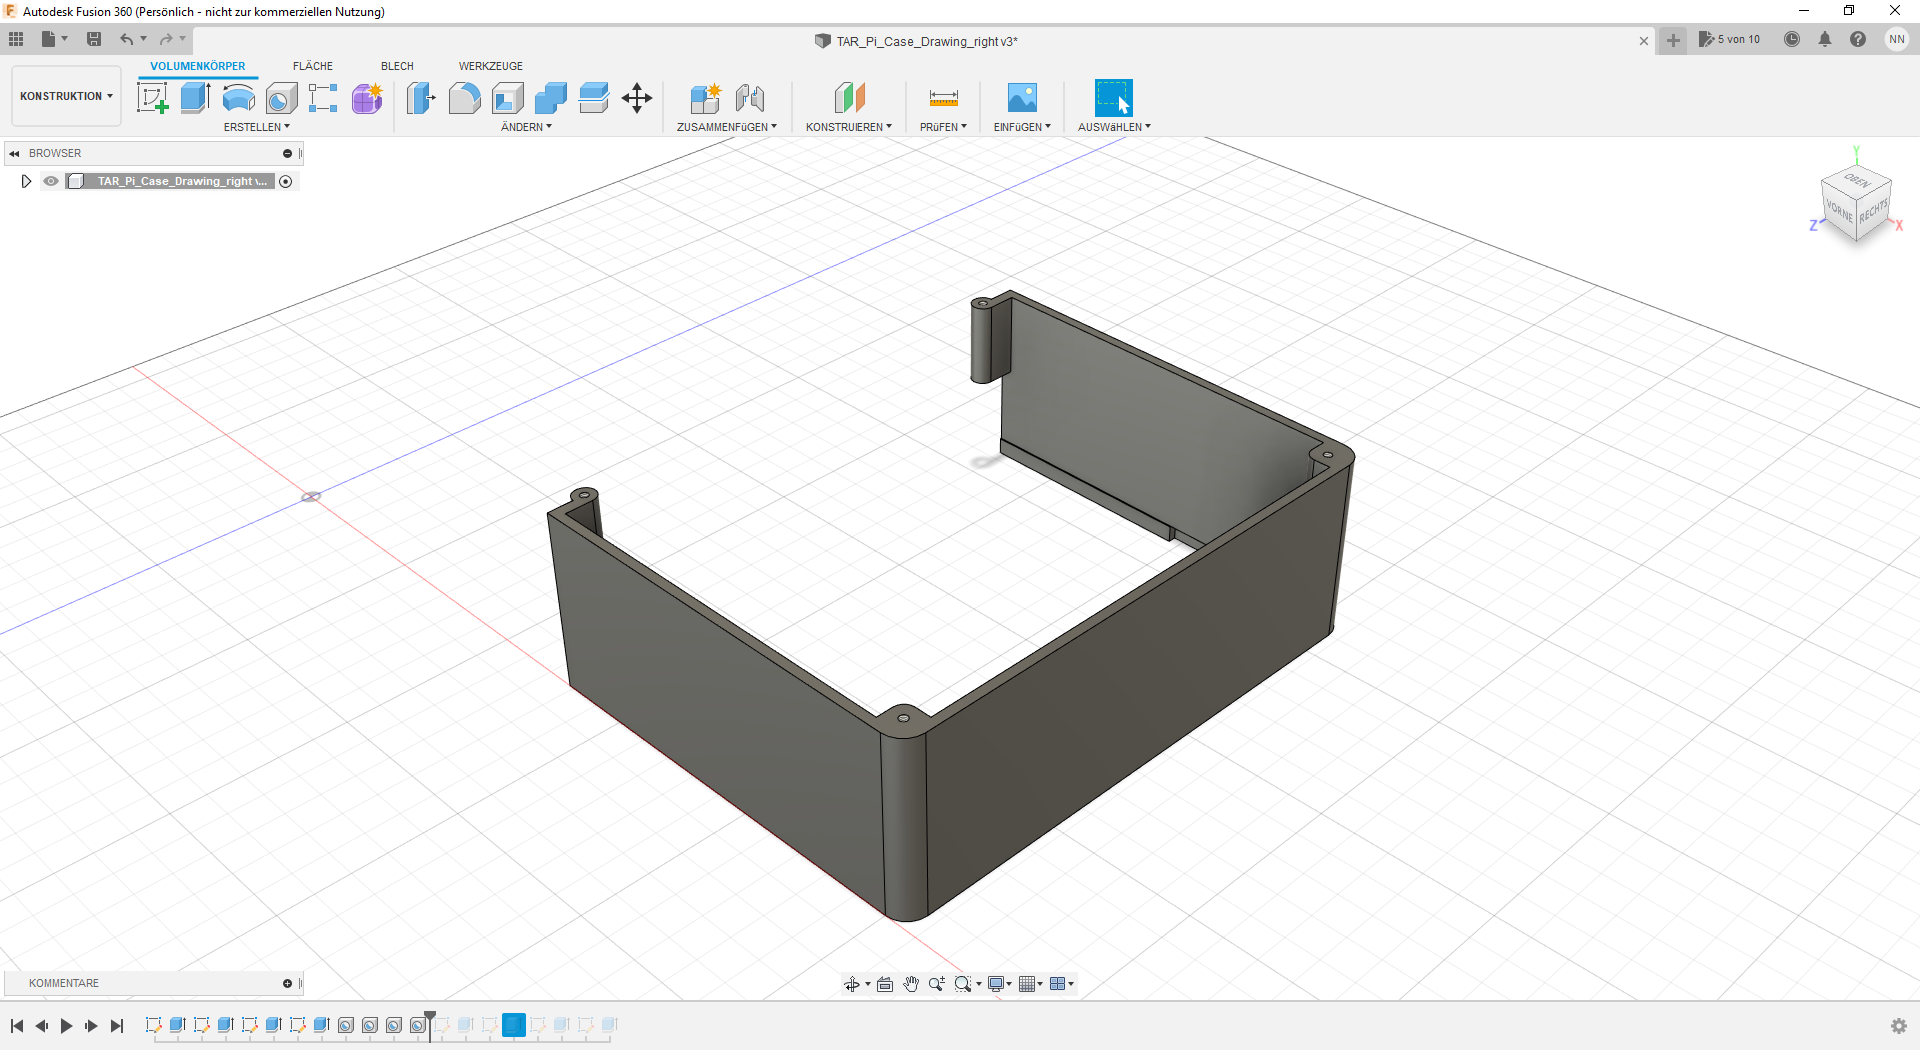
\includegraphics[width=\linewidth]{img/konstruktion_gehaeuse_rechts_008.png}
		\caption[Bohrung für Schrauben]{Bohrung für Schrauben}
		\label{fig:design-right-08}
	\end{subfigure}
	\begin{subfigure}[t]{.3\linewidth}
		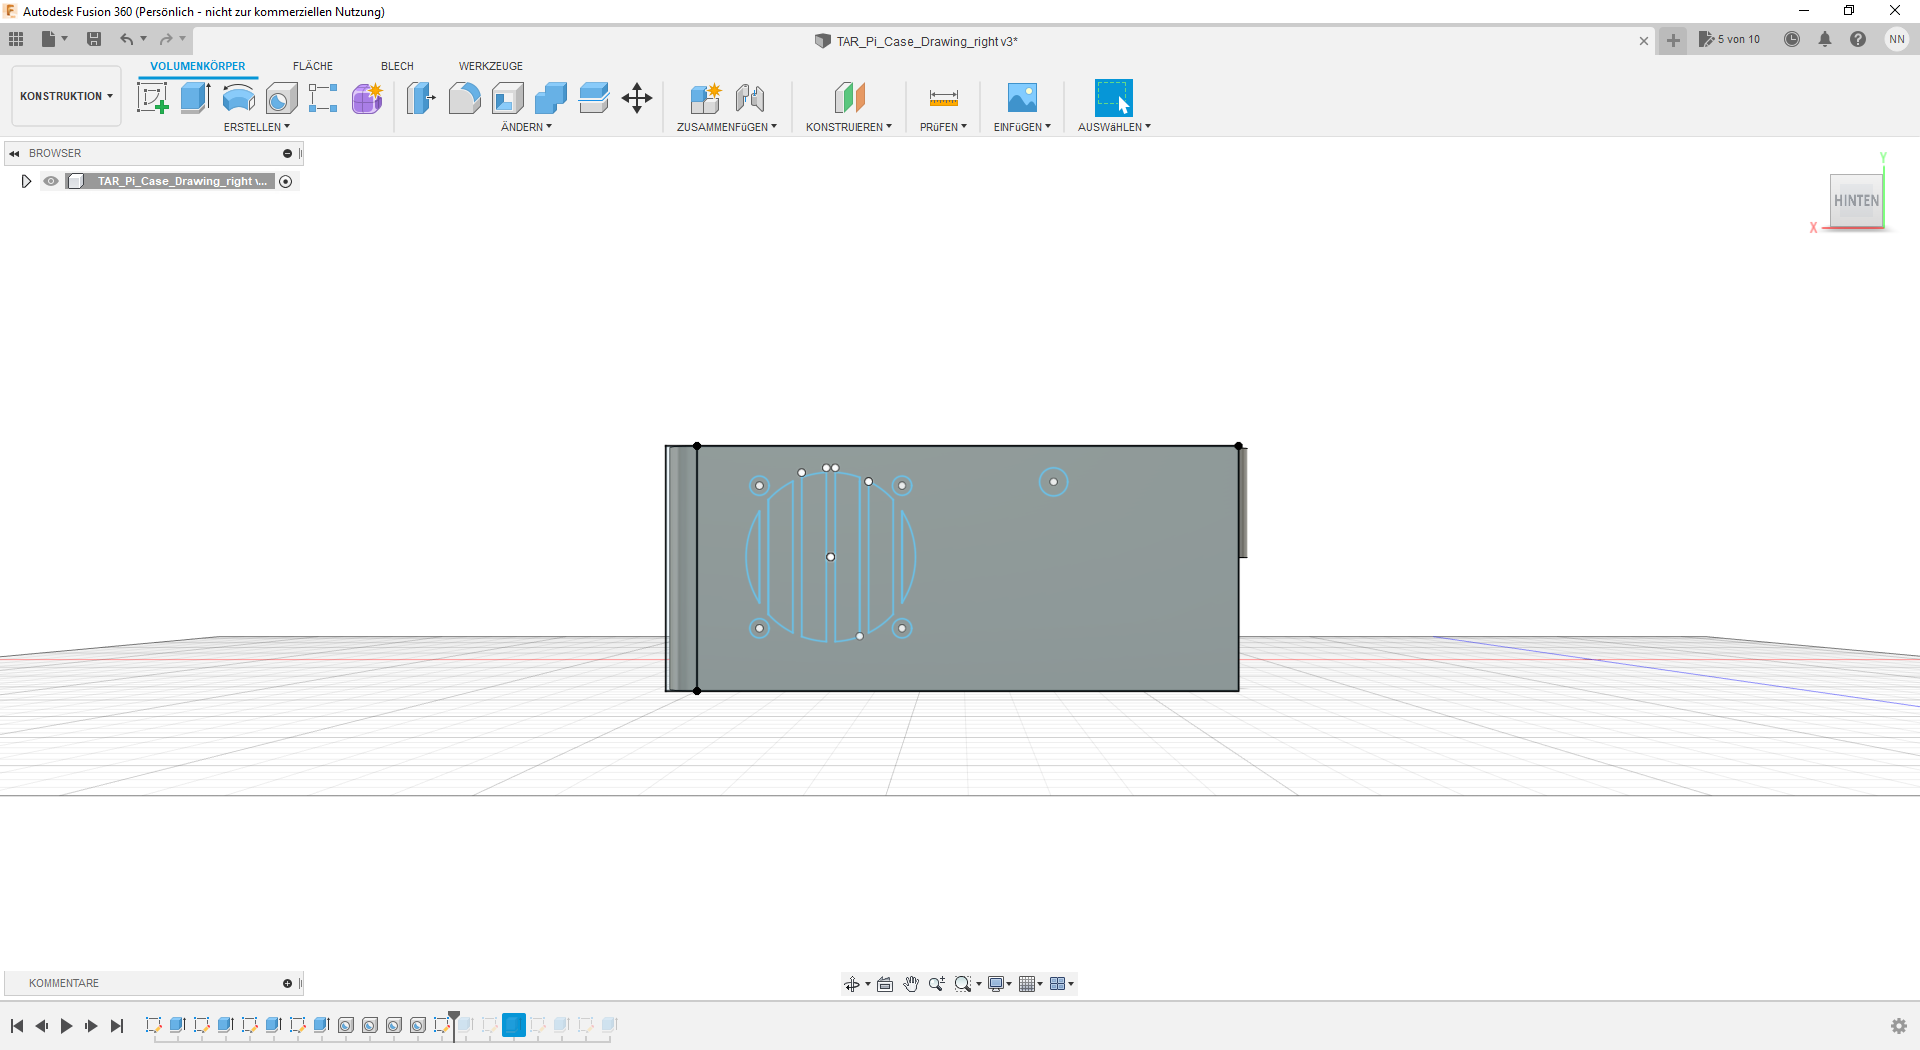
\includegraphics[width=\linewidth]{img/konstruktion_gehaeuse_rechts_009.png}
		\caption[Zeichnung für Lüfteröffnung \& Antennenausgang]{Zeichnung für Lüfteröffnung \& Antennenausgang}
		\label{fig:design-right-09}
	\end{subfigure}
	\begin{subfigure}[t]{.3\linewidth}
		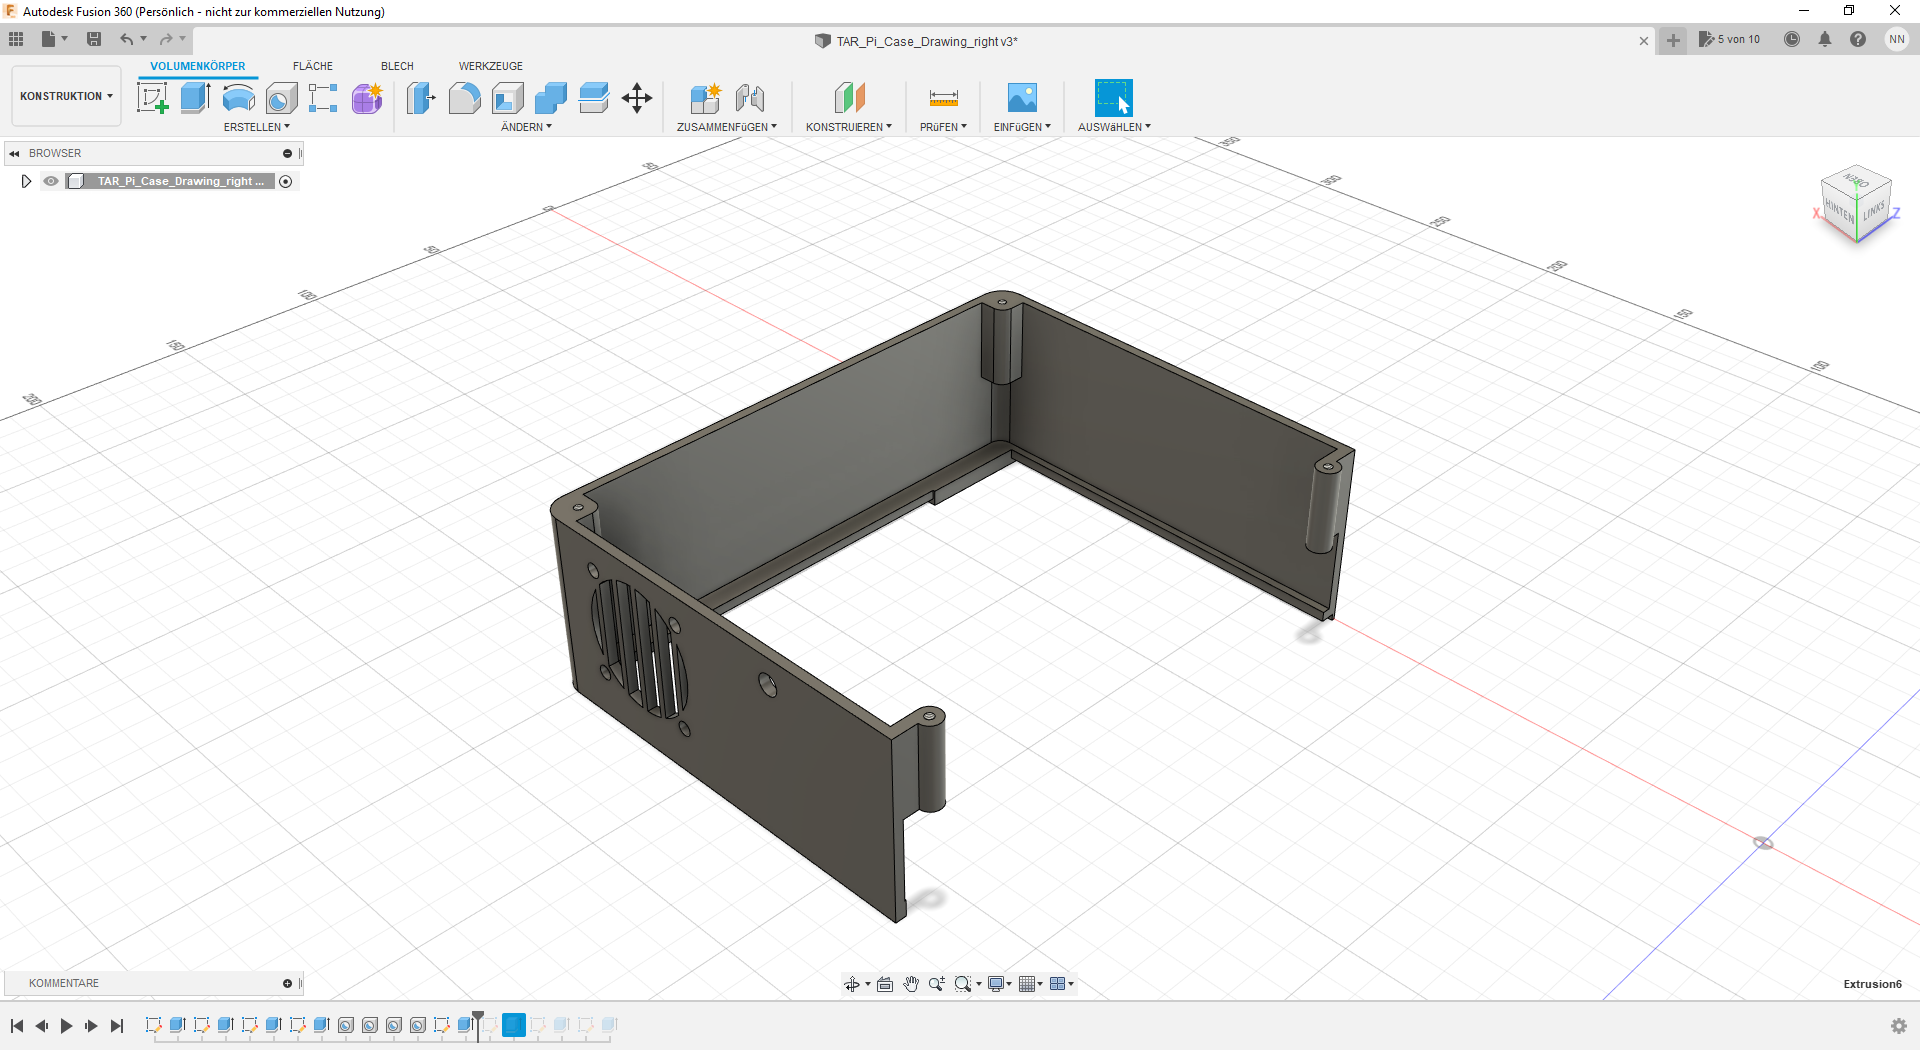
\includegraphics[width=\linewidth]{img/konstruktion_gehaeuse_rechts_010.png}
		\caption[Extrusion der Lüfteröffnung]{Extrusion der Lüfteröffnung}
		\label{fig:design-right-10}
	\end{subfigure}
	\begin{subfigure}[t]{.3\linewidth}
		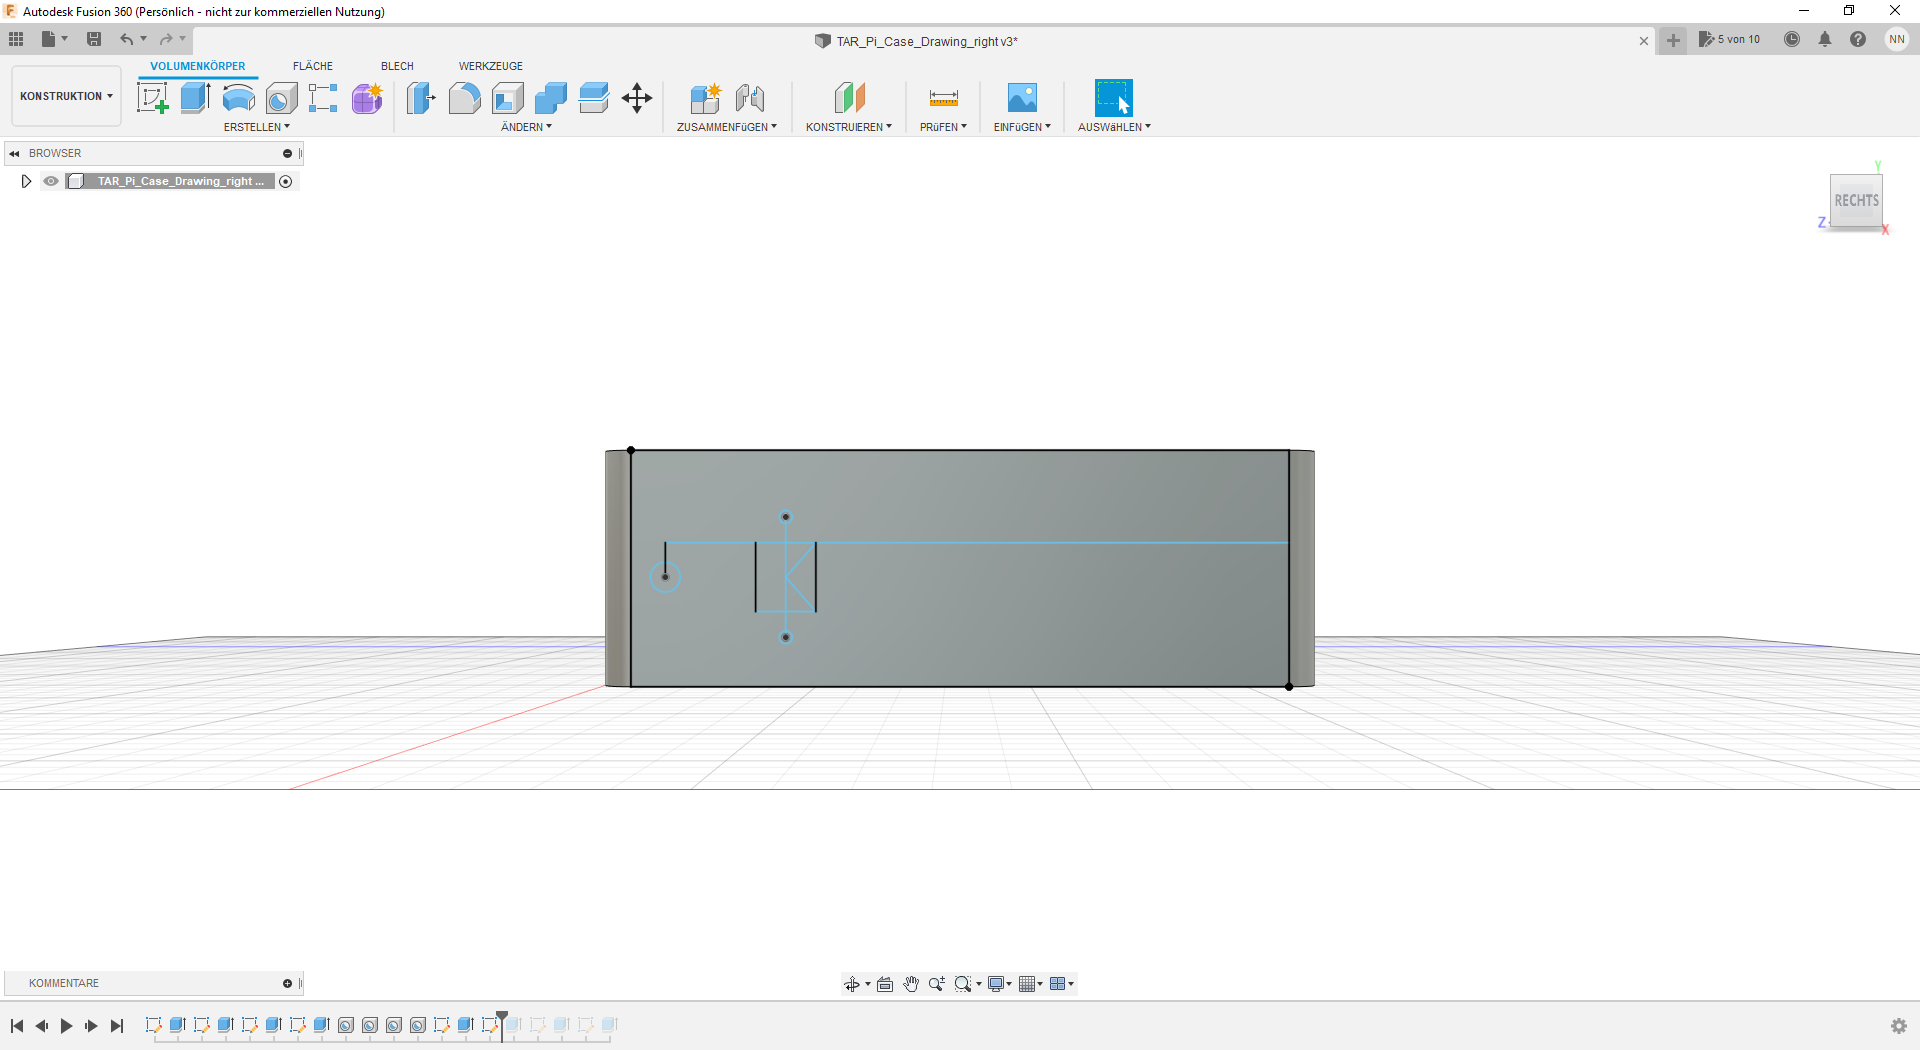
\includegraphics[width=\linewidth]{img/konstruktion_gehaeuse_rechts_011.png}
		\caption[Zeichnung der Aussparung für Stromanschluss \& Netzwerkbuchse]{Zeichnung der Aussparung für Stromanschluss \& Netzwerkbuchse}
		\label{fig:design-right-11}
	\end{subfigure}
	\begin{subfigure}[t]{.3\linewidth}
		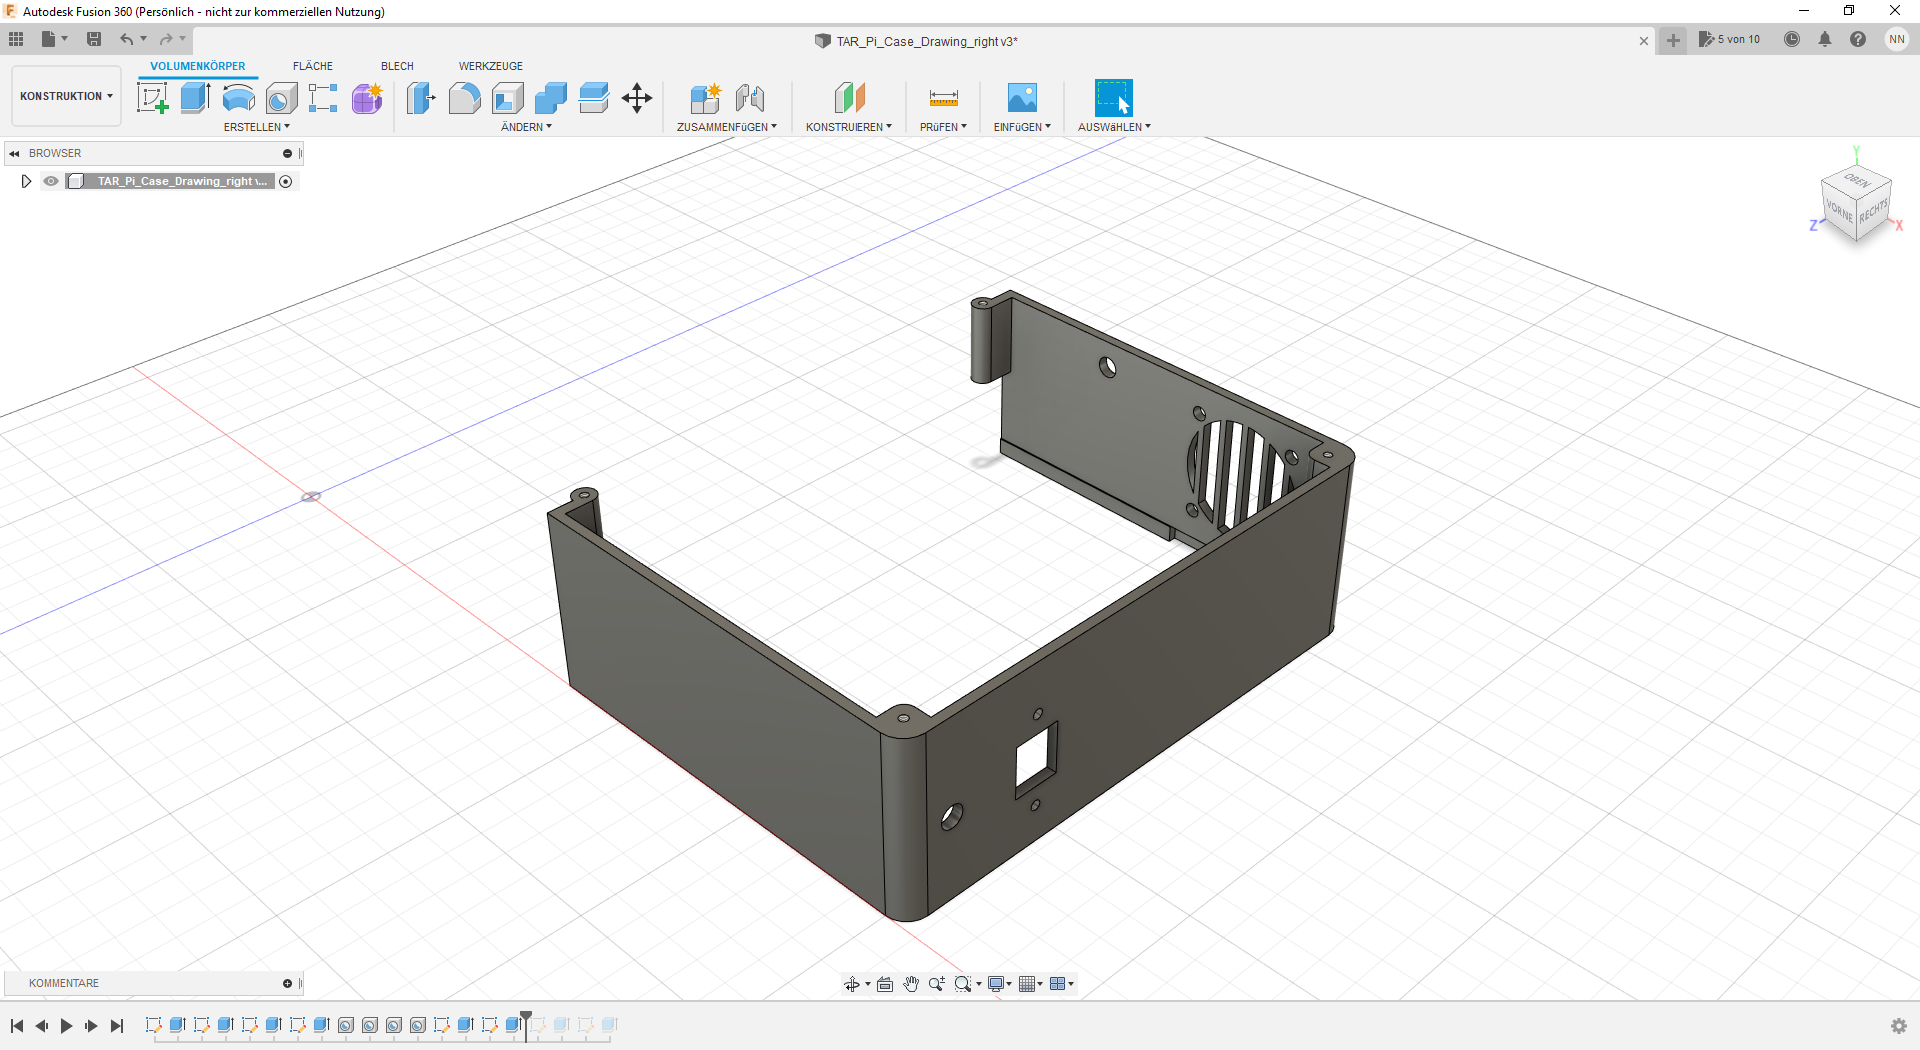
\includegraphics[width=\linewidth]{img/konstruktion_gehaeuse_rechts_012.png}
		\caption[Extrusion der Netzwerkbuchse]{Extrusion der Netzwerkbuchse}
		\label{fig:design-right-12}
	\end{subfigure}
	\begin{subfigure}[t]{.3\linewidth}
		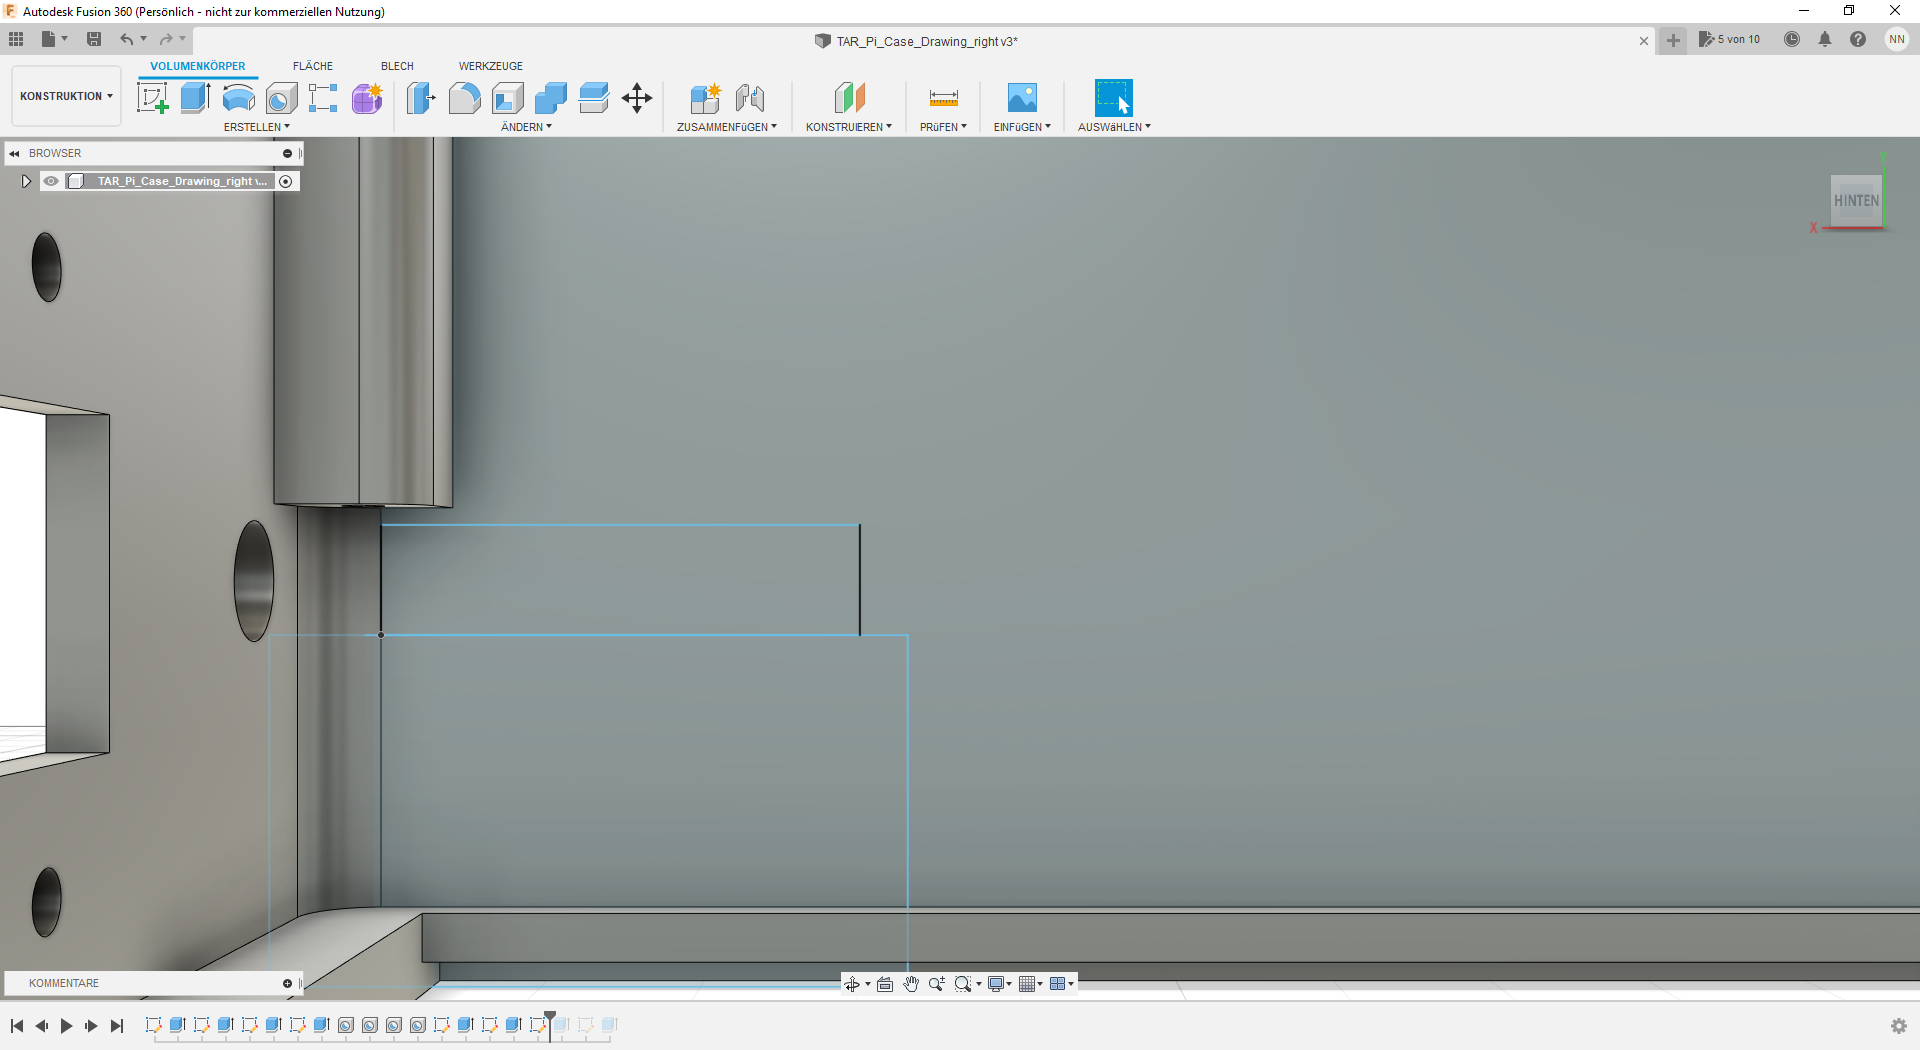
\includegraphics[width=\linewidth]{img/konstruktion_gehaeuse_rechts_013.png}
		\caption[Zeichnung des Stromsteckerblocks]{Zeichnung des Stromsteckerblocks}
		\label{fig:design-right-13}
	\end{subfigure}
	\begin{subfigure}[t]{.3\linewidth}
		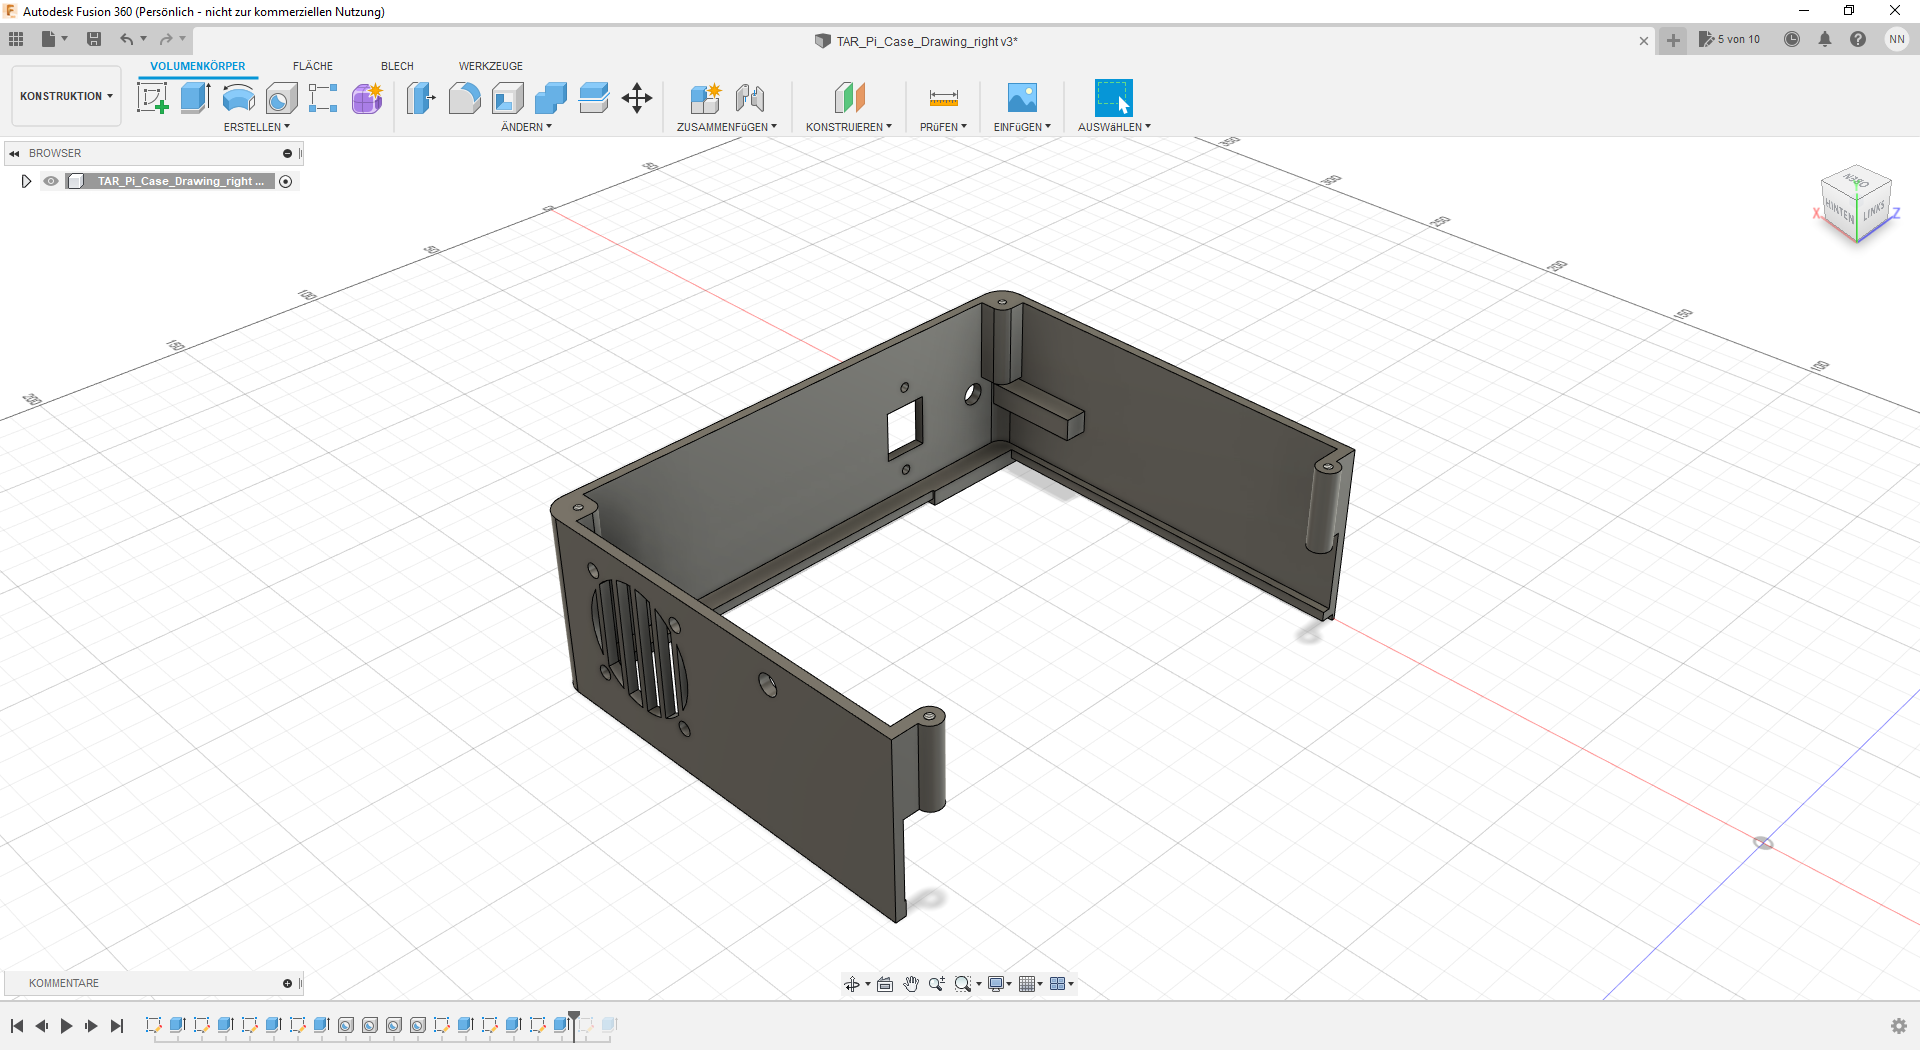
\includegraphics[width=\linewidth]{img/konstruktion_gehaeuse_rechts_014.png}
		\caption[Extrusion des Stromsteckerblocks]{Extrusion des Stromsteckerblocks}
		\label{fig:design-right-14}
	\end{subfigure}
	\begin{subfigure}[t]{.3\linewidth}
		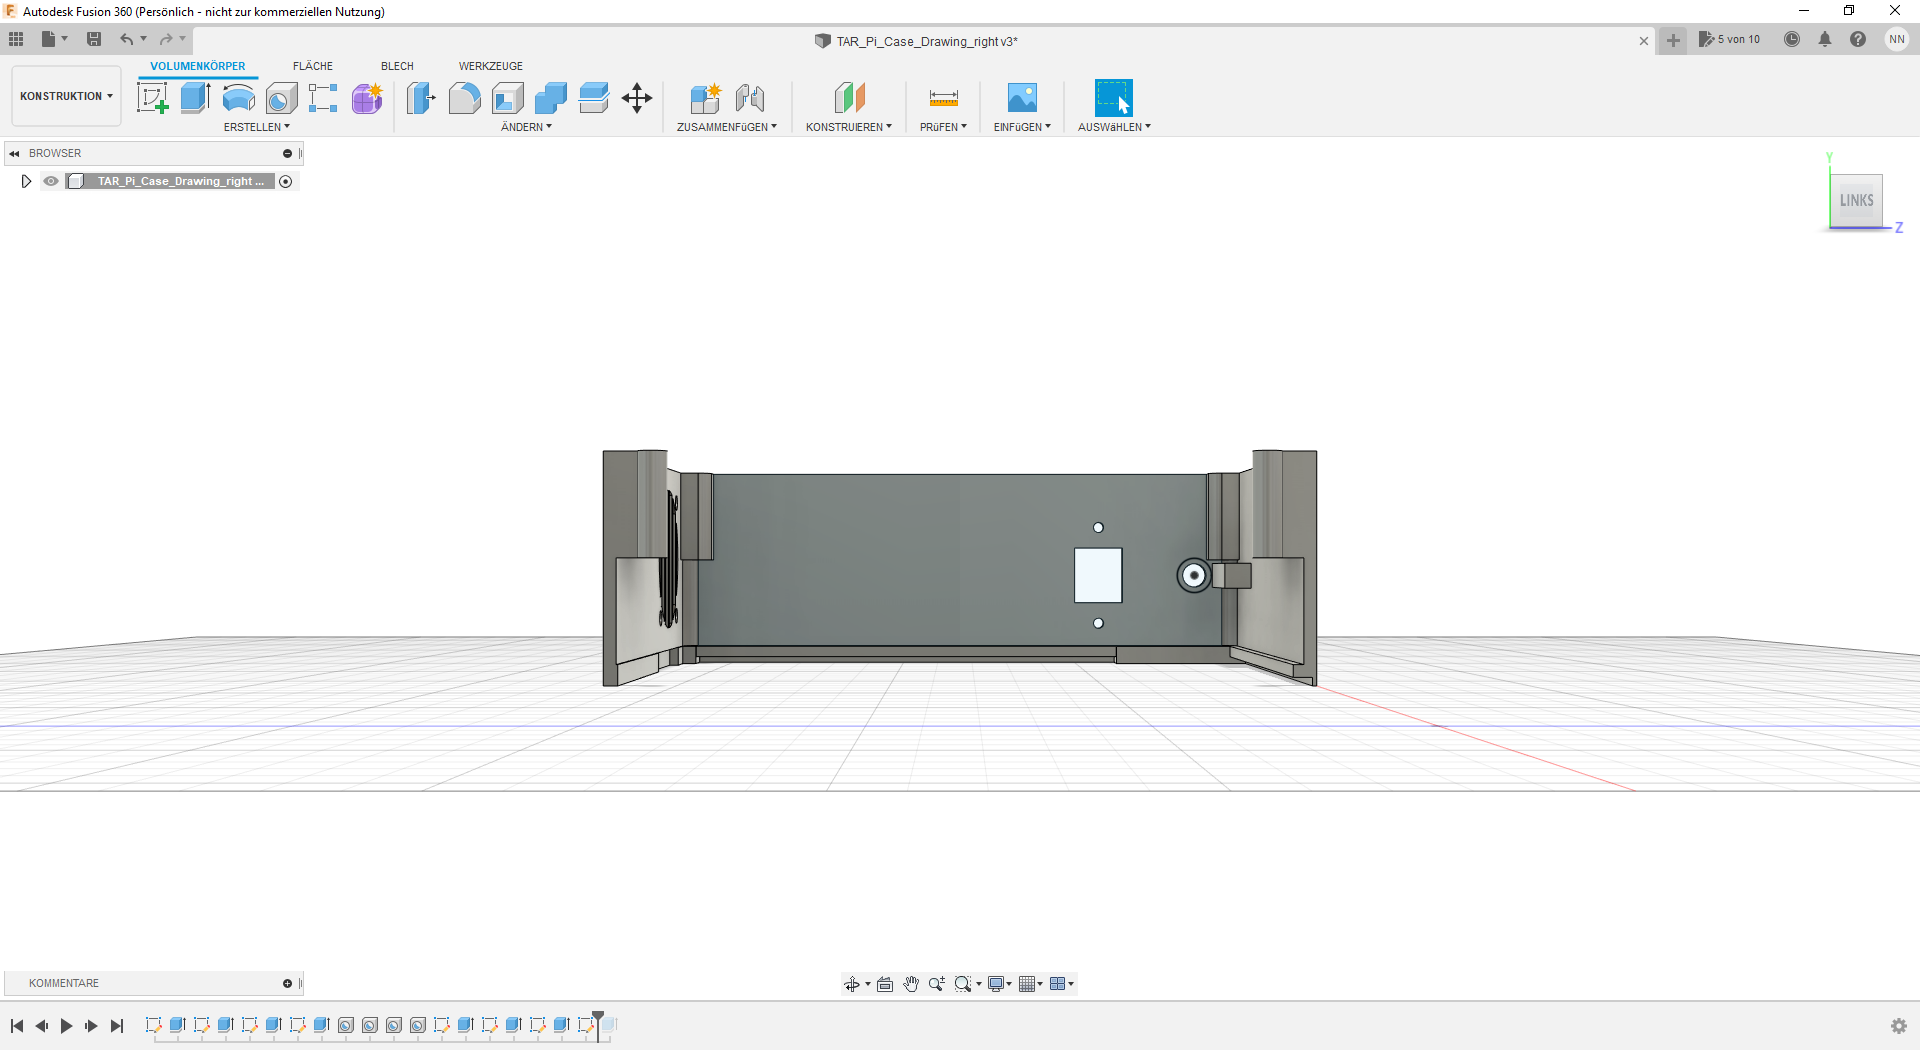
\includegraphics[width=\linewidth]{img/konstruktion_gehaeuse_rechts_015.png}
		\caption[Zeichnung der Aussparung]{Zeichnung der Aussparung}
		\label{fig:design-right-15}
	\end{subfigure}
	\begin{subfigure}[t]{.3\linewidth}
		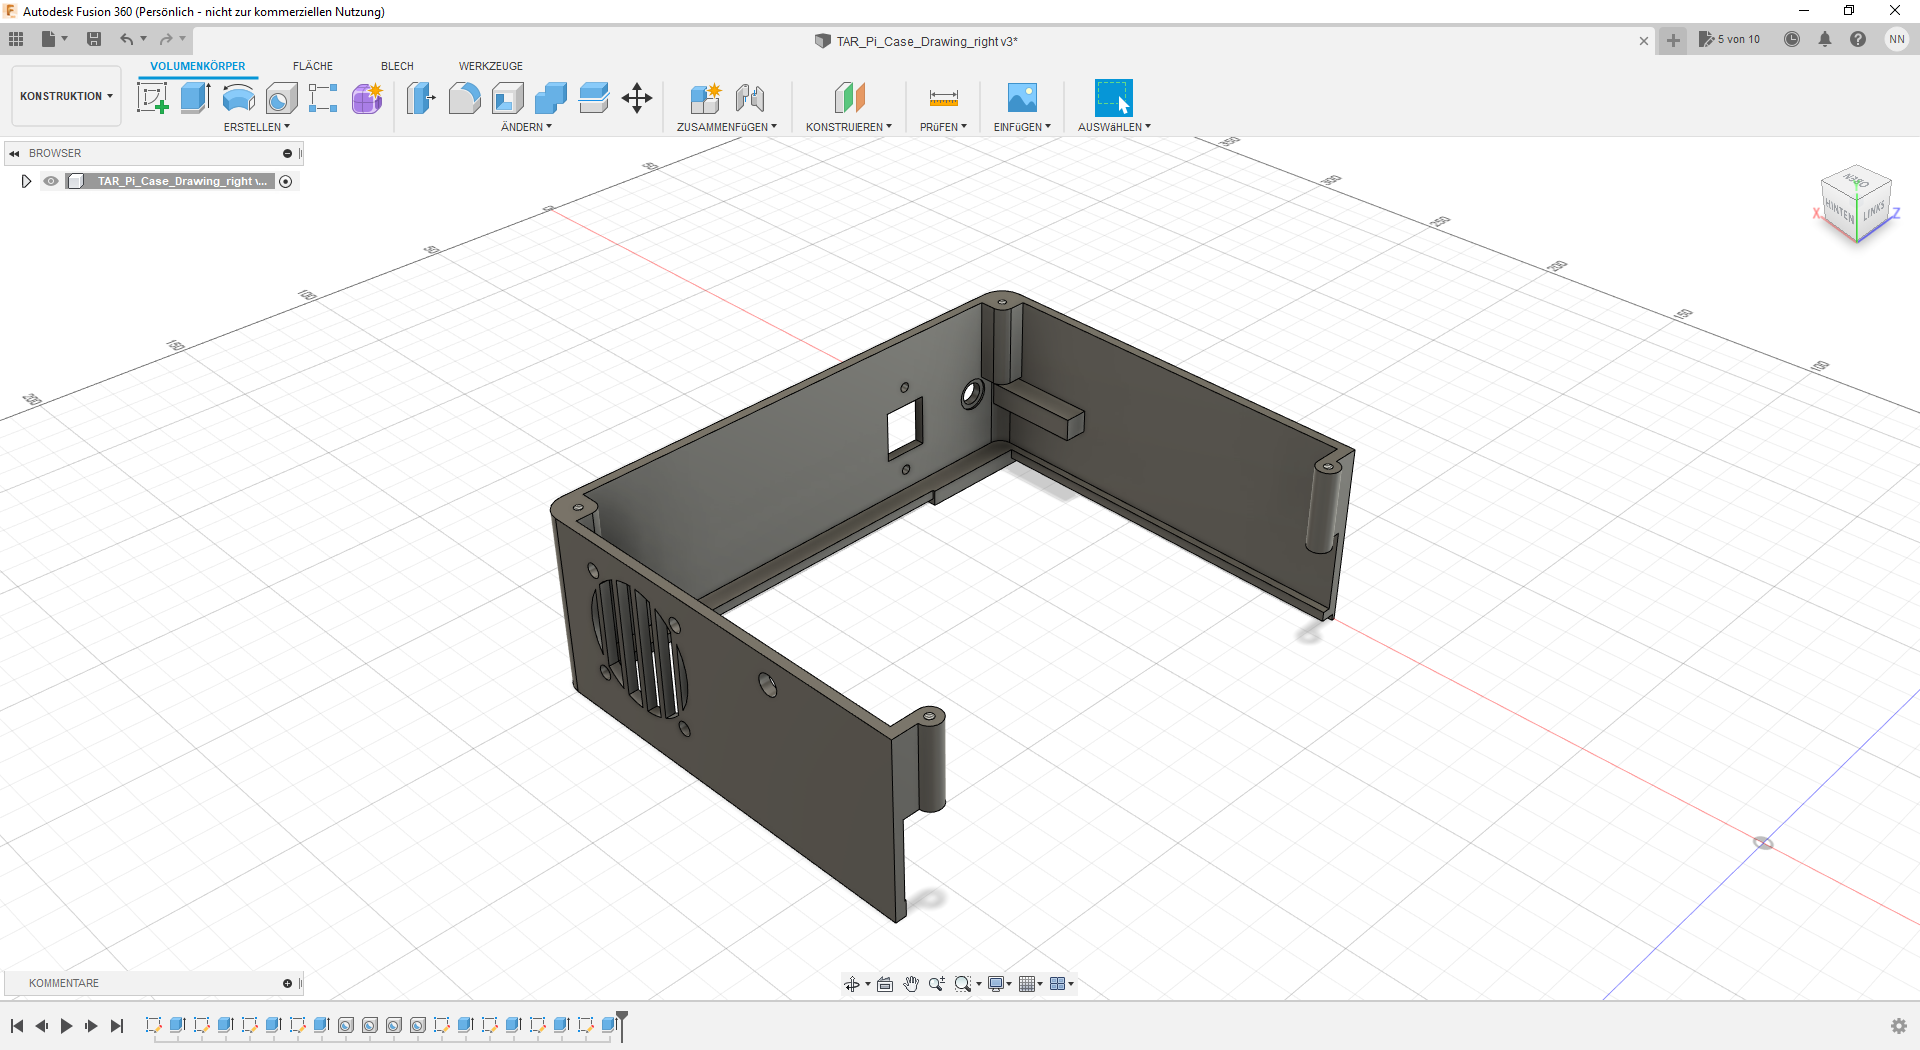
\includegraphics[width=\linewidth]{img/konstruktion_gehaeuse_rechts_016.png}
		\caption[Extrusion der Aussparung]{Extrusion der Aussparung}
		\label{fig:design-right-16}
	\end{subfigure}
	\caption[Entwurf des rechten Wandteils]{Entwurf des rechten Wandteils}
	\label{fig:design-right}
\end{figure}\par
\paragraph{Gehäuserückwand}\par
Das Design der Gehäuserückwand basiert nur rudimentär auf der in Abb. \ref{fig:design-case-base}: \nameref{fig:design-case-base} erstellten Zeichnung. 
Die Außenmaße stimmen zwar überein, die Zeichnung für die Auflage auf den Seitenwänden haben wir aber neu erstellt. 
Zusätzlich haben wir eine Diagonale zur punktsymmetrischen Trennung der Teile eingefügt (vgl. Abb. \ref{fig:design-back-01}: \nameref{fig:design-back-01}), welche den Zeitaufwand für den Druck von zwei unterschiedlichen Teilen für die Rückseite reduzieren soll. \\
\noindent Nachdem wir die  Zeichnung extrudiert haben (vgl. Abb. \ref{fig:design-back-02}: \nameref{fig:design-back-02}), haben wir noch einen Vorsprung auf der kurzen Seite des Bauteils extrudiert (vgl. Abb. \ref{fig:design-back-03}: \nameref{fig:design-back-03}), um die beiden Rückwandteile besser verbinden zu können. 
Anschließend haben wir ein weiter Teil der inneren Zeichnung ins Negative extrudiert, um diesen Bereich freizustellen (vgl. Abb. \ref{fig:design-back-04}: \nameref{fig:design-back-04}) und um beim Druck der Teile Material zu sparen. \\
\noindent Damit für eventuelle Toleranzen zwischen den beiden Teilen Platz ist, haben wir auf dem Vorsprung die Aussparung für die darunterliegende Schraubendurchführung erhöht (vgl. Abb. \ref{fig:design-back-05}: \nameref{fig:design-back-05}) und den Vorsprung von unten mit einer Fase versehen, was den Materialverbrauch für das Teil weiter reduziert (vgl. Abb. \ref{fig:design-back-06}: \nameref{fig:design-back-06}). 
Zudem haben wir die obere Kante (vgl. Abb. \ref{fig:design-back-07}: \nameref{fig:design-back-07}), die Innenseite (vgl. Abb. \ref{fig:design-back-08}: \nameref{fig:design-back-08}) und auch den Vorsprung (vgl. Abbildung \ref{fig:design-back-09}: \nameref{fig:design-back-09}) mit einer Fase versehen. \\
\noindent Um die Bohrungen an die richtige Stellen setzen zu können, haben wir eine Hilfszeichnung auf die Außenfläche, also die Außenseite der Rückwand, aufgelegt (vgl. Abb. \ref{fig:design-back-10}: \nameref{fig:design-back-10}). 
Dort haben wir dann drei M3-Bohrungen für Senkkopfschrauben gesetzt (vgl. Abb. \ref{fig:design-back-11}: \nameref{fig:design-back-11}). \\
\noindent Für die Aufhängungen auf der Rückseite des Gehäuses haben wir eine weitere Zeichnung aufgelegt (vgl. Abb. \ref{fig:design-back-12}: \nameref{fig:design-back-12}) und dann ins Negativ extrudiert (vgl. Abb. \ref{fig:design-back-13}: \nameref{fig:design-back-13}).
So kann das Gehäuse mit zwei Schrauben an der Wand angebracht werden.  
Um beim Aufhängen nicht an einen bestimmten Typ Schrauben gebunden zu sein, haben wir eine kleine Fase an den engeren Teil der Aufhängungen gelegt (vgl. Abb. \ref{fig:design-back-14}: \nameref{fig:design-back-14}). 
\begin{figure}[H]
	\begin{subfigure}[t]{.3\linewidth}
		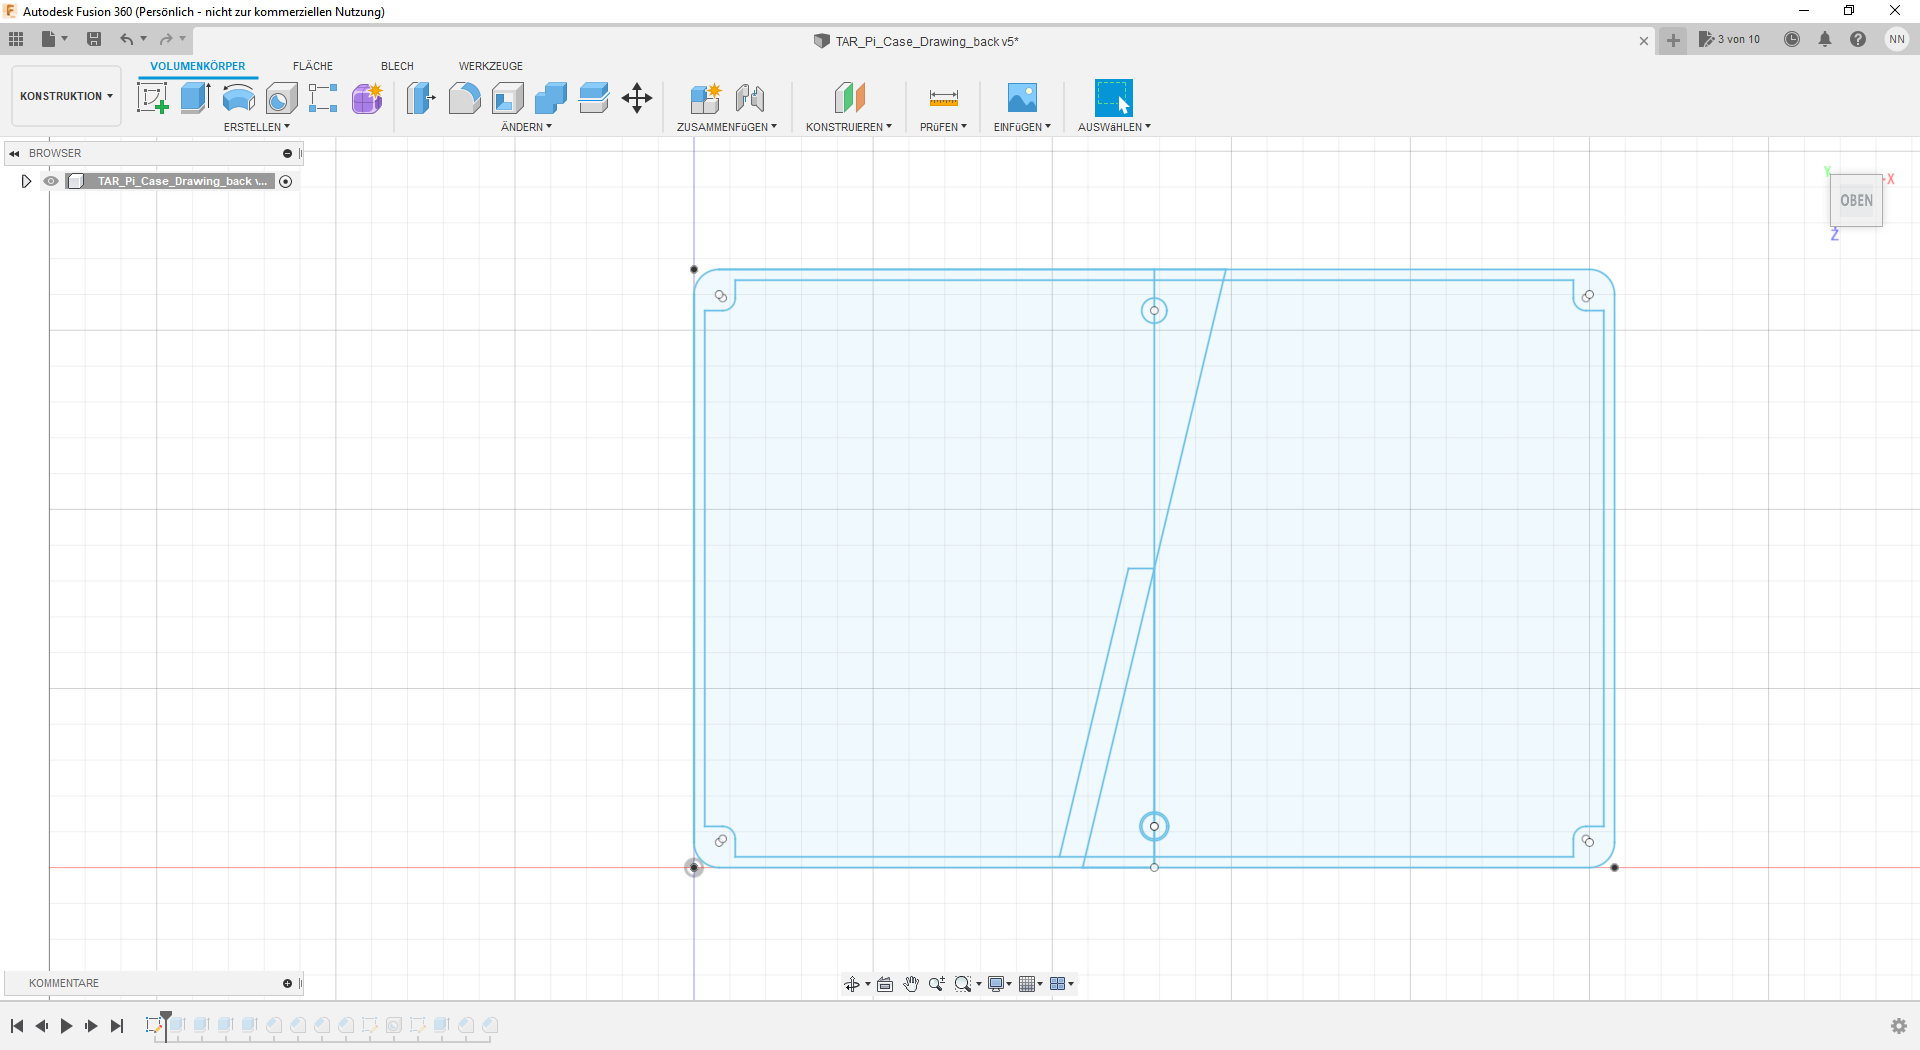
\includegraphics[width=\linewidth]{img/konstruktion_gehaeuse_hinten_001.png}
		\caption[Grundrisszeichnung]{Grundrisszeichnung}
		\label{fig:design-back-01}
	\end{subfigure}	
	\begin{subfigure}[t]{.3\linewidth}
		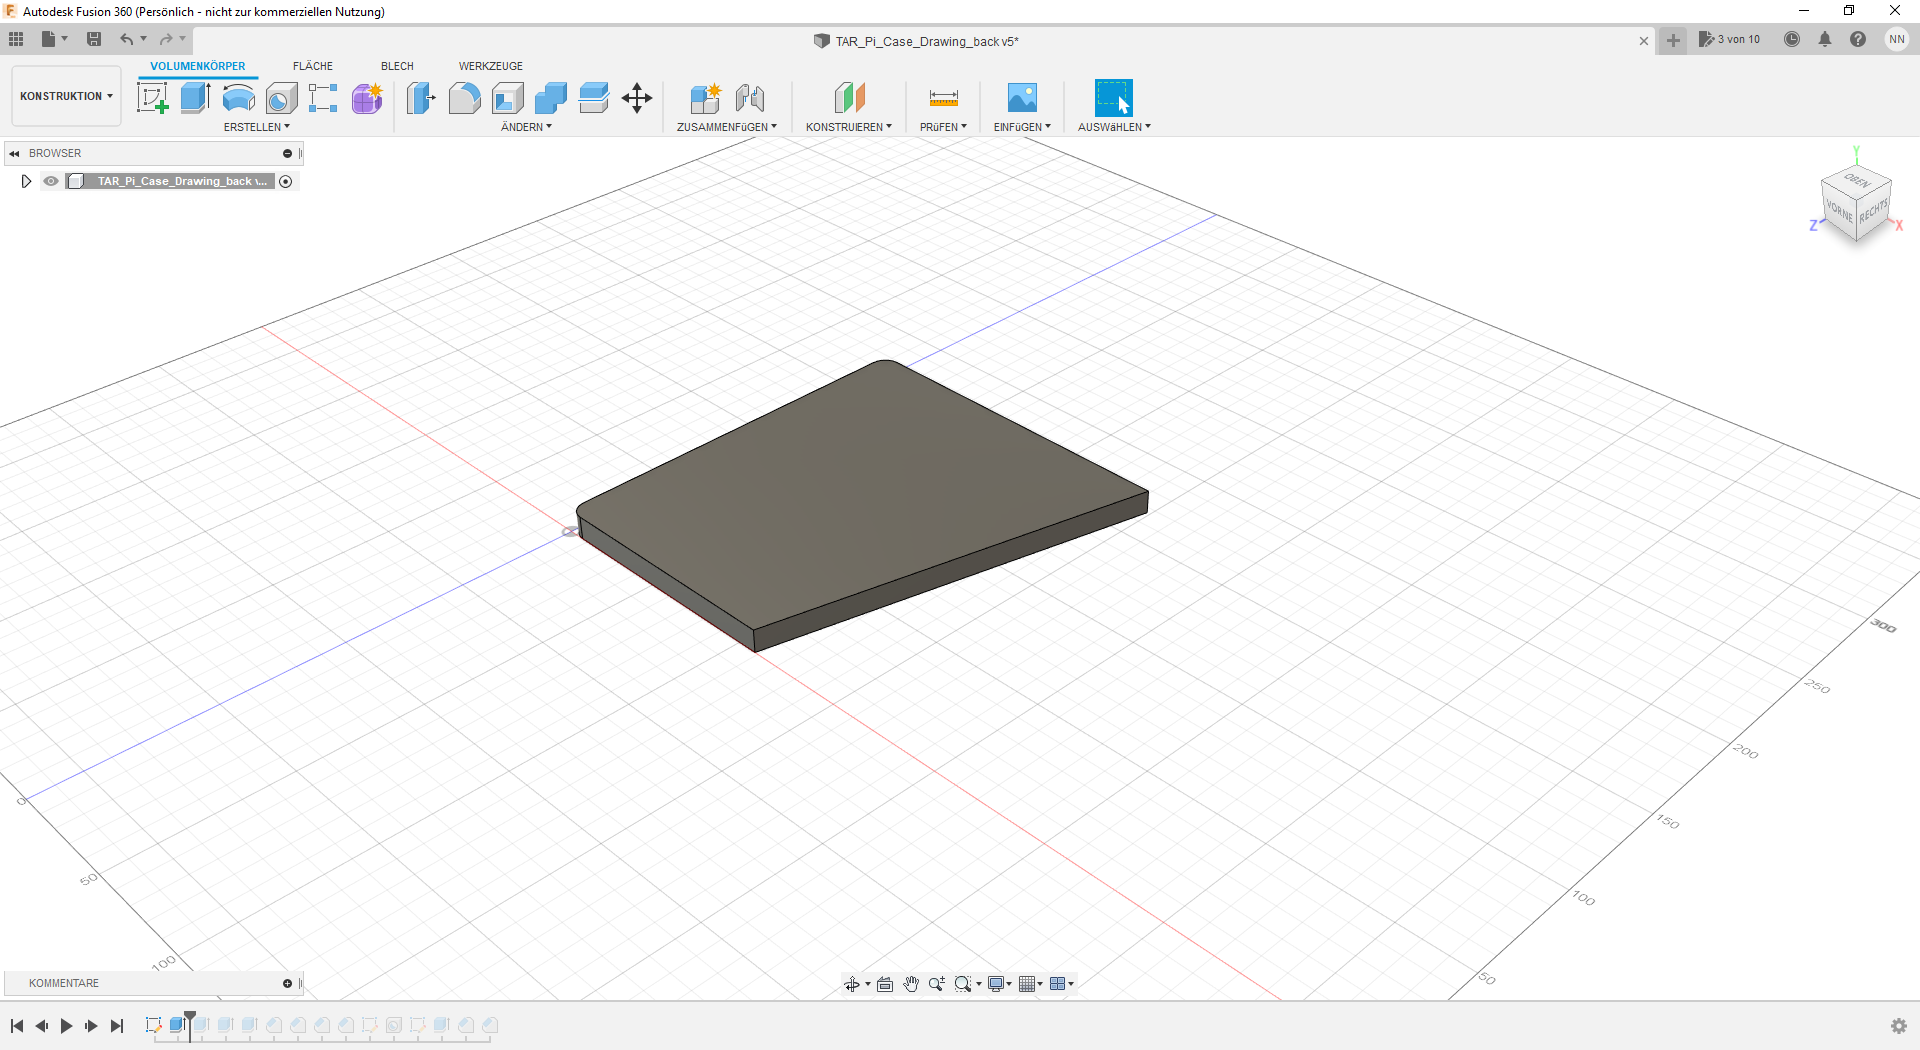
\includegraphics[width=\linewidth]{img/konstruktion_gehaeuse_hinten_002.png}
		\caption[Extrusion der Grundform]{Extrusion der Grundform}
		\label{fig:design-back-02}
	\end{subfigure}
	\begin{subfigure}[t]{.3\linewidth}
		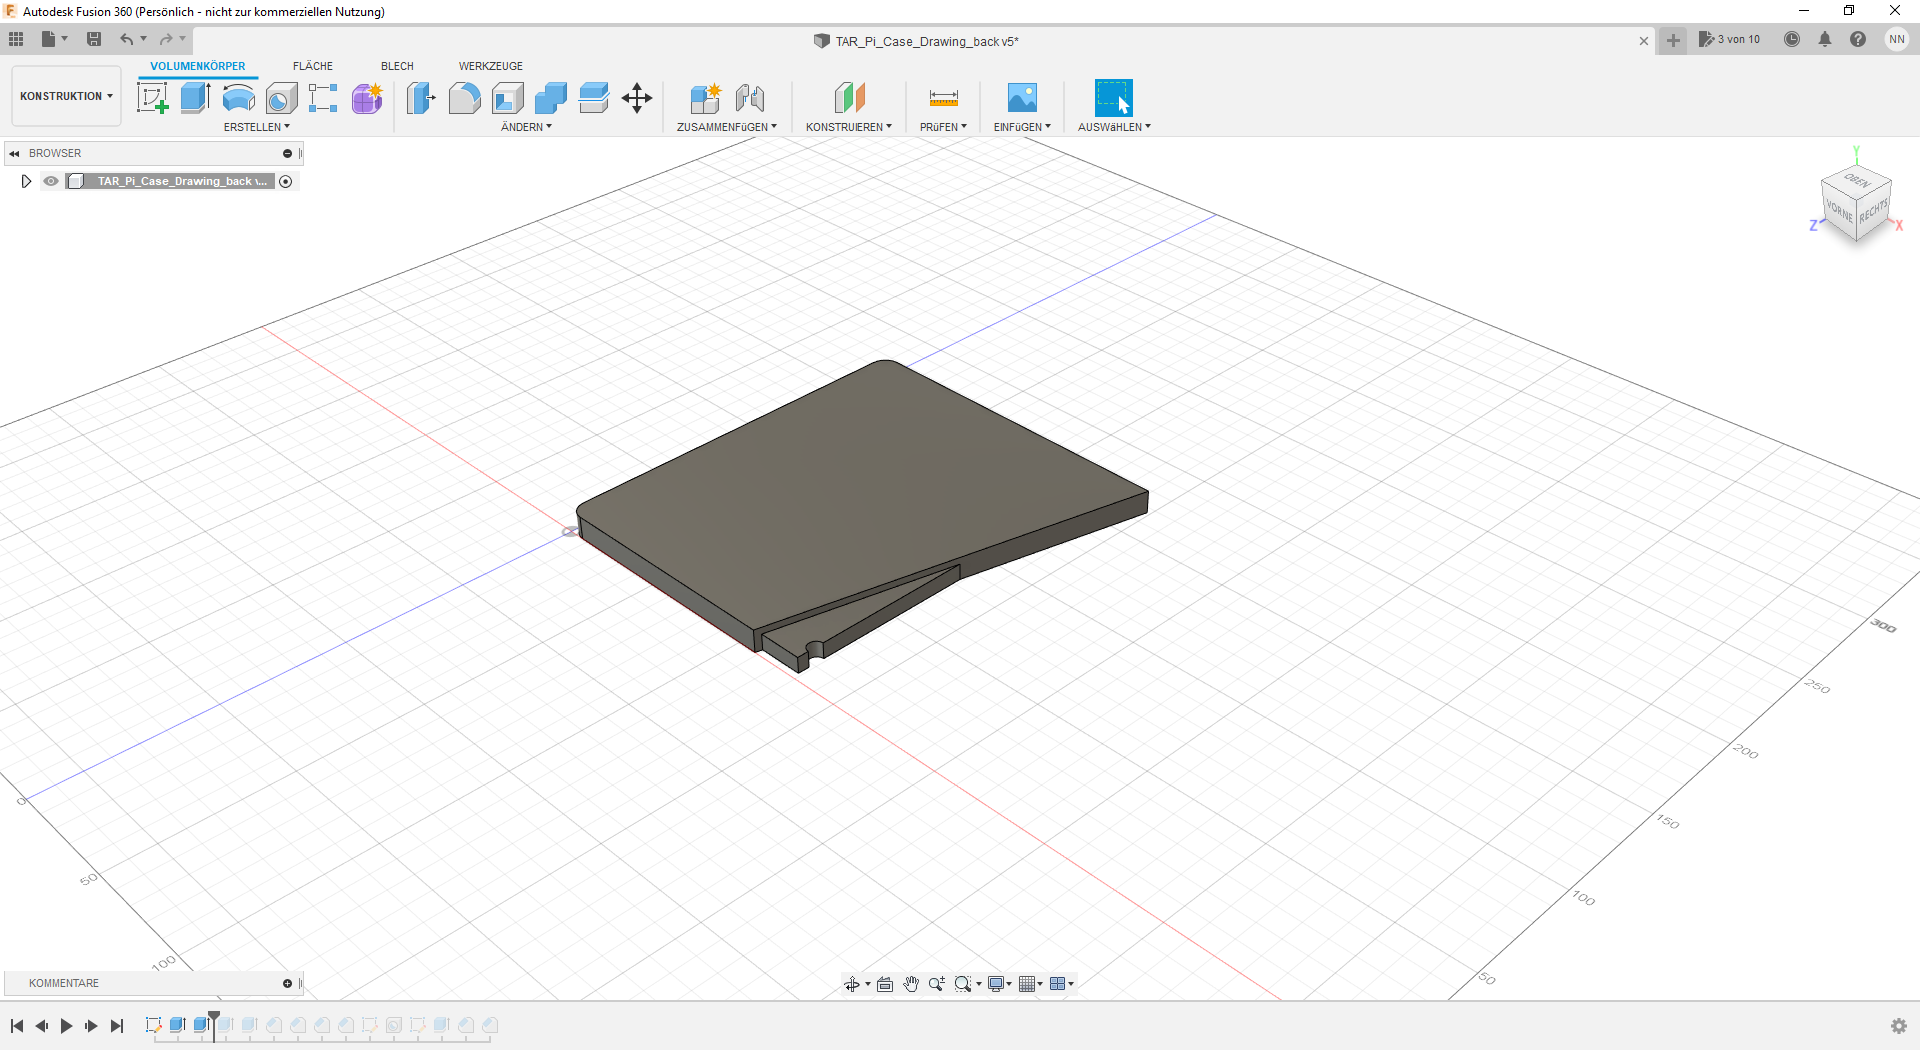
\includegraphics[width=\linewidth]{img/konstruktion_gehaeuse_hinten_003.png}
		\caption[Extrusion des Vorsprungs]{Extrusion des Vorsprungs}
		\label{fig:design-back-03}
	\end{subfigure}
	\begin{subfigure}[t]{.3\linewidth}
		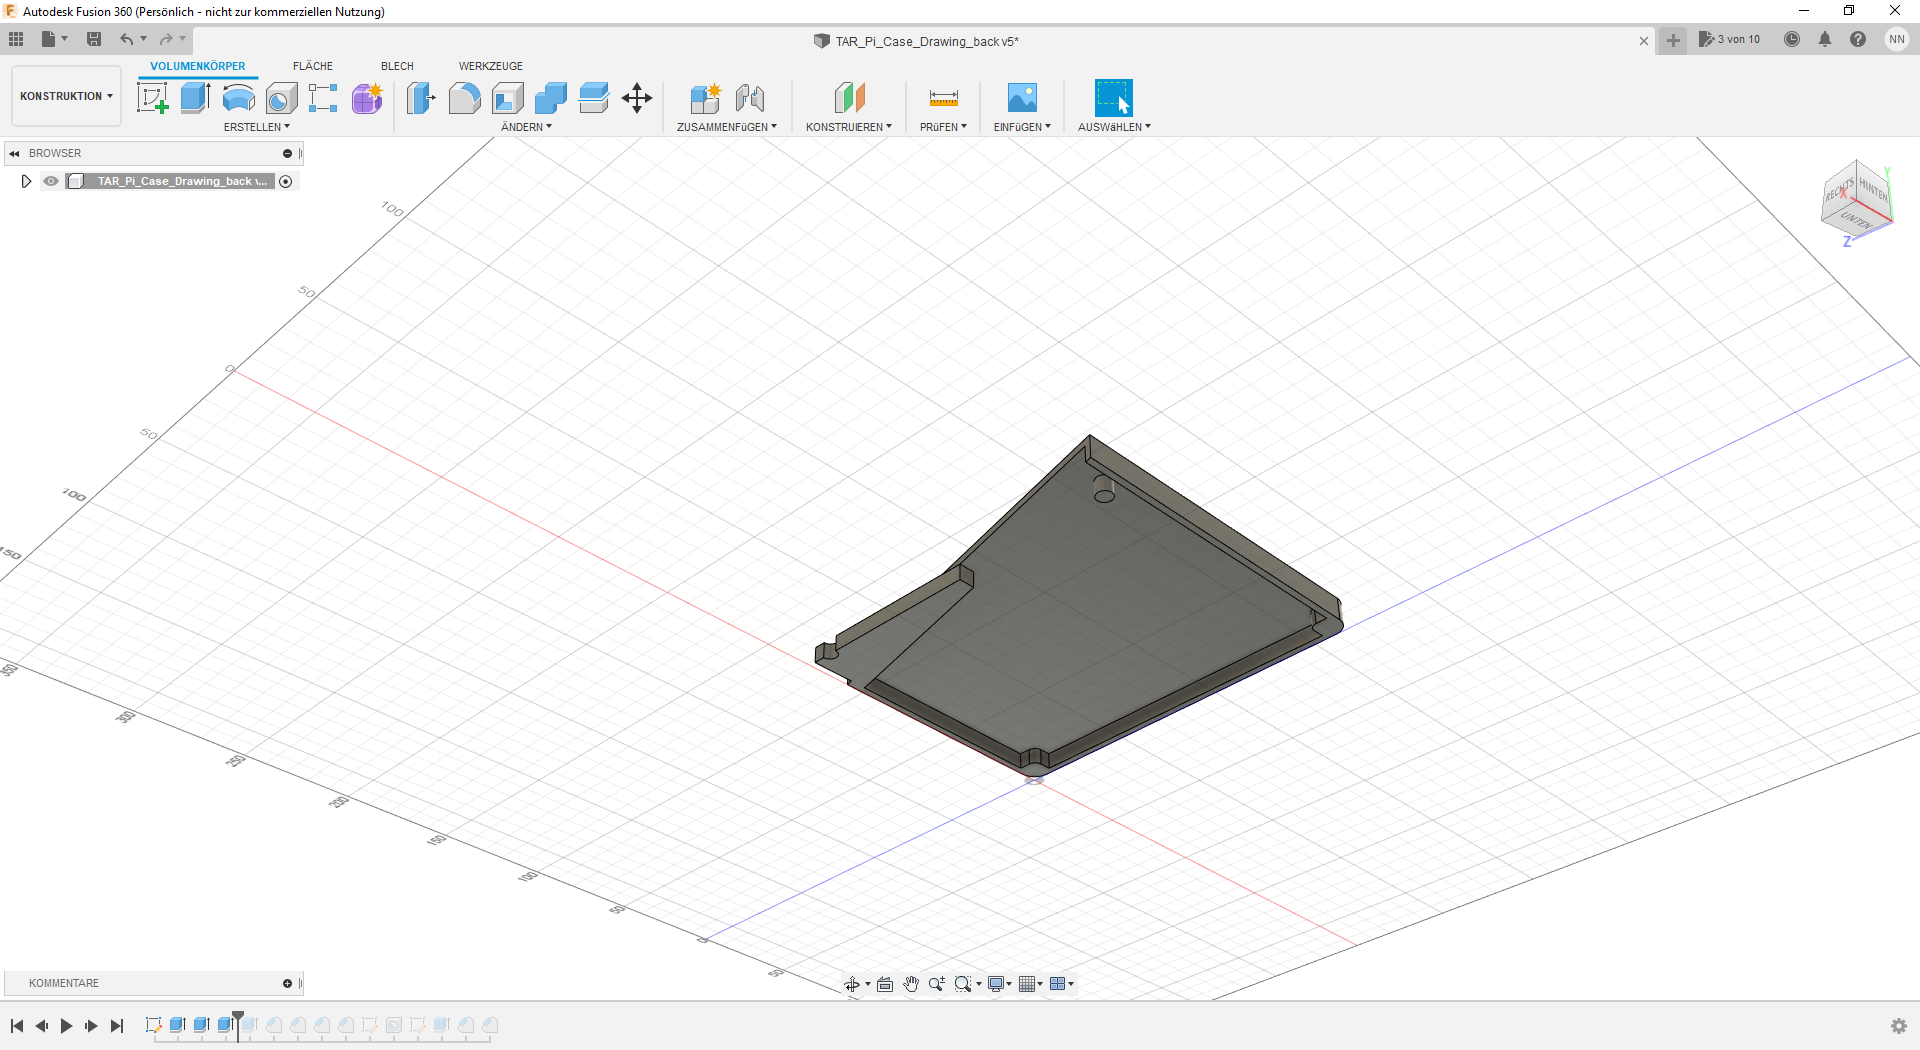
\includegraphics[width=\linewidth]{img/konstruktion_gehaeuse_hinten_004.png}
		\caption[Erstellen der Aussparung]{Erstellen der Aussparung}
		\label{fig:design-back-04}
	\end{subfigure}
	\begin{subfigure}[t]{.3\linewidth}
		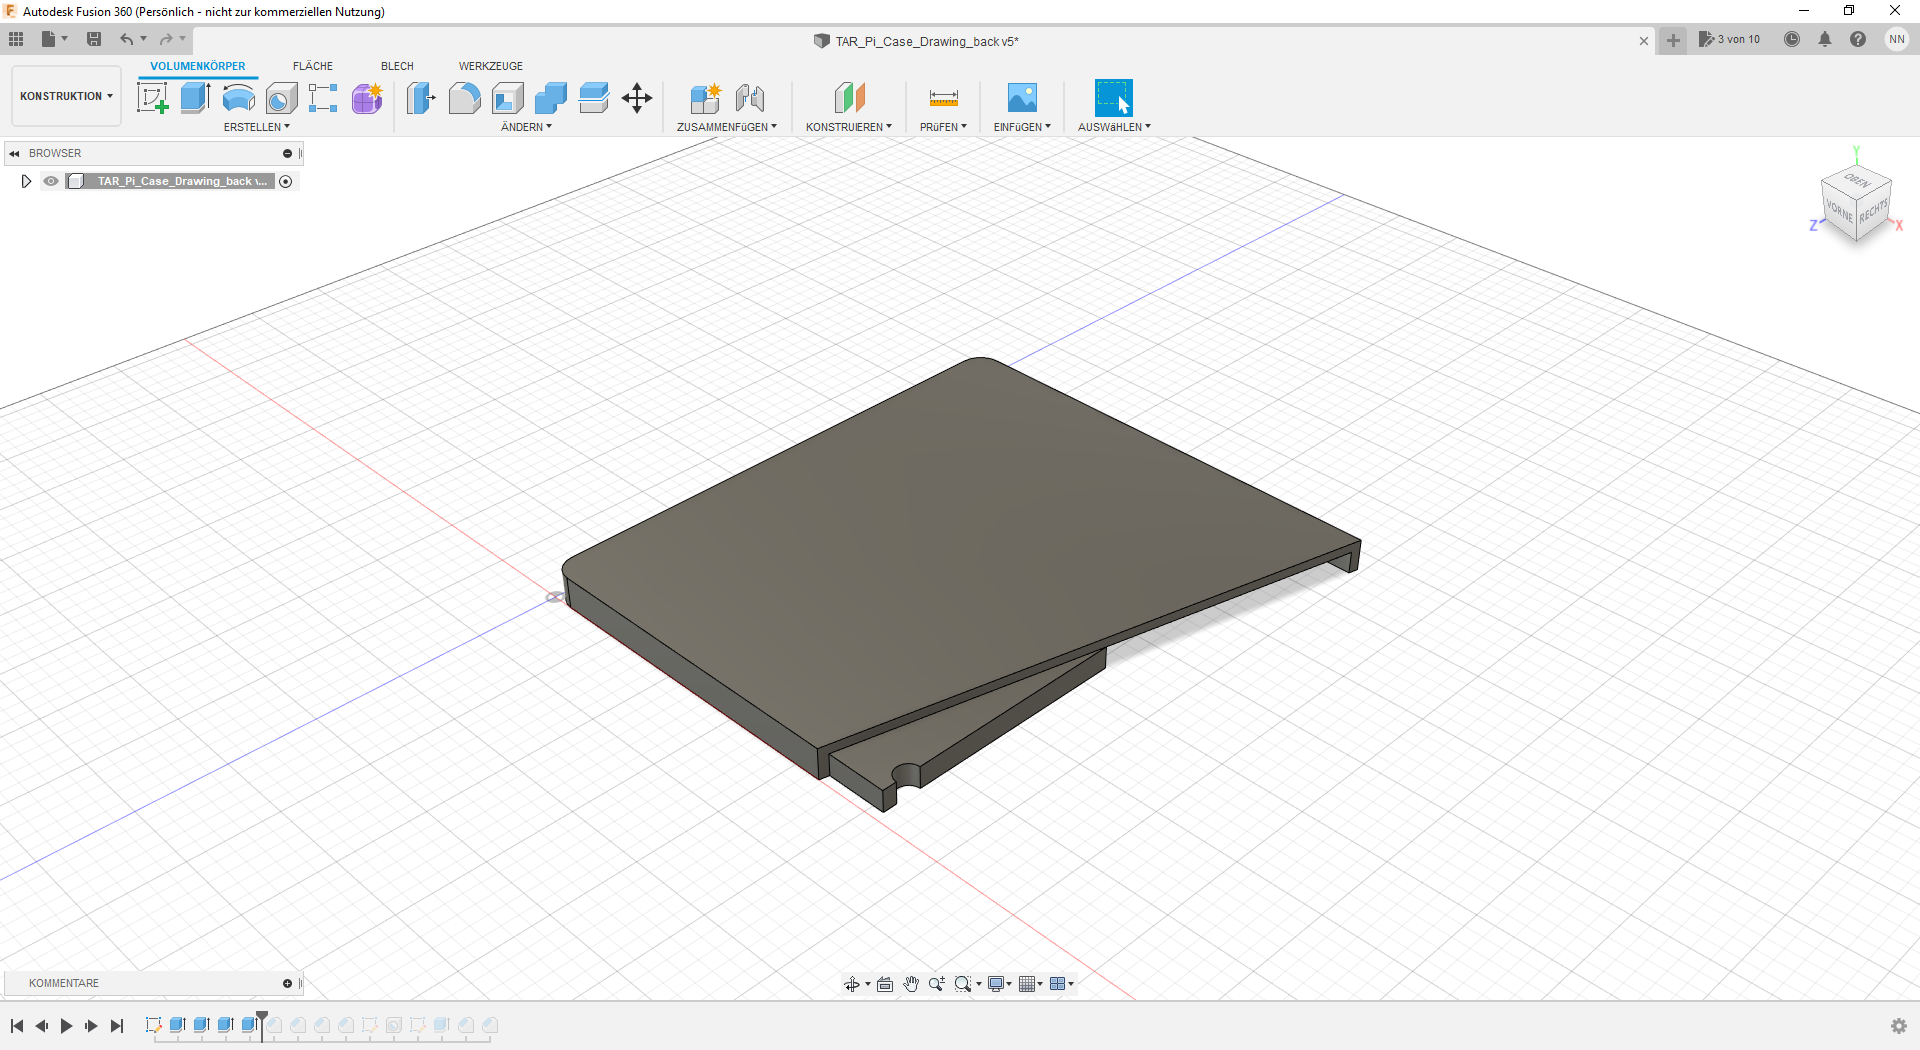
\includegraphics[width=\linewidth]{img/konstruktion_gehaeuse_hinten_005.png}
		\caption[Anpassung für Toleranz]{Anpassung für Toleranz}
		\label{fig:design-back-05}
	\end{subfigure}
	\begin{subfigure}[t]{.3\linewidth}
		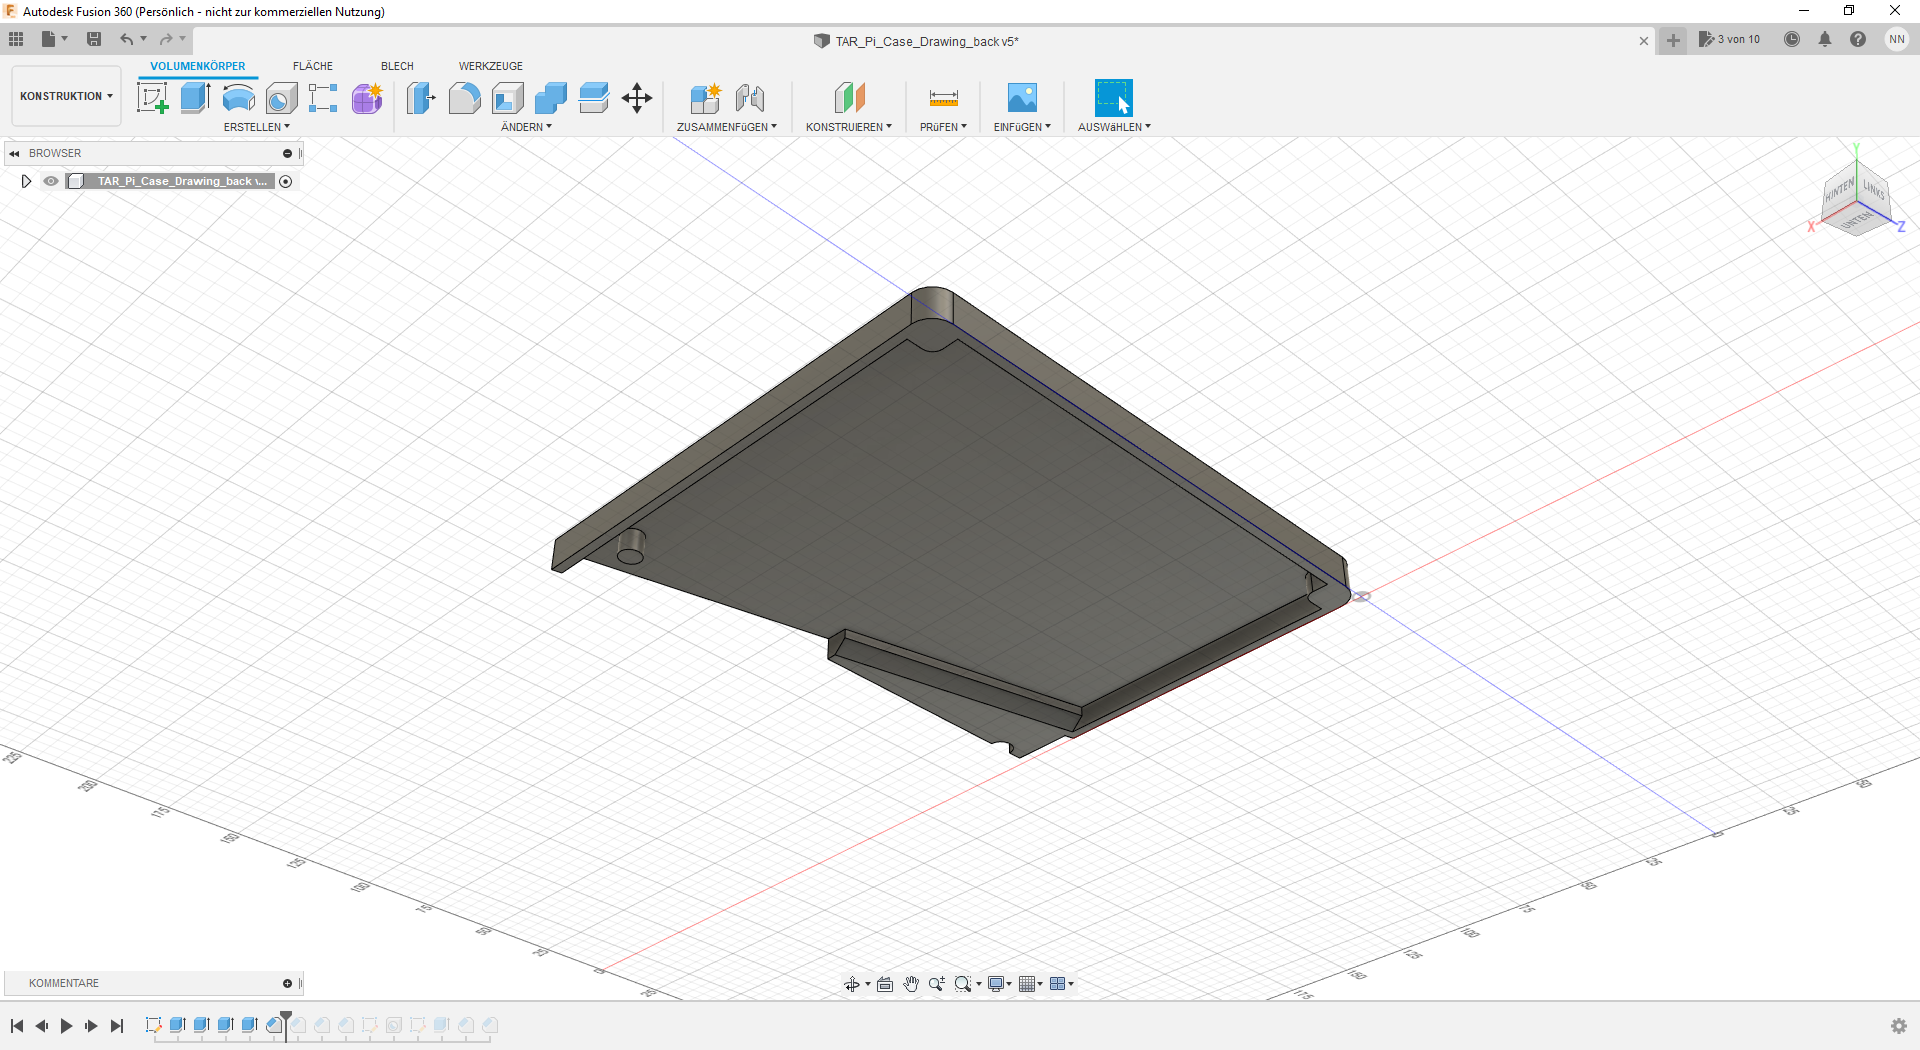
\includegraphics[width=\linewidth]{img/konstruktion_gehaeuse_hinten_006.png}
		\caption[Abfasen des Vorsprungs]{Abfasen des Vorsprungs}
		\label{fig:design-back-06}
	\end{subfigure}
	\begin{subfigure}[t]{.3\linewidth}
		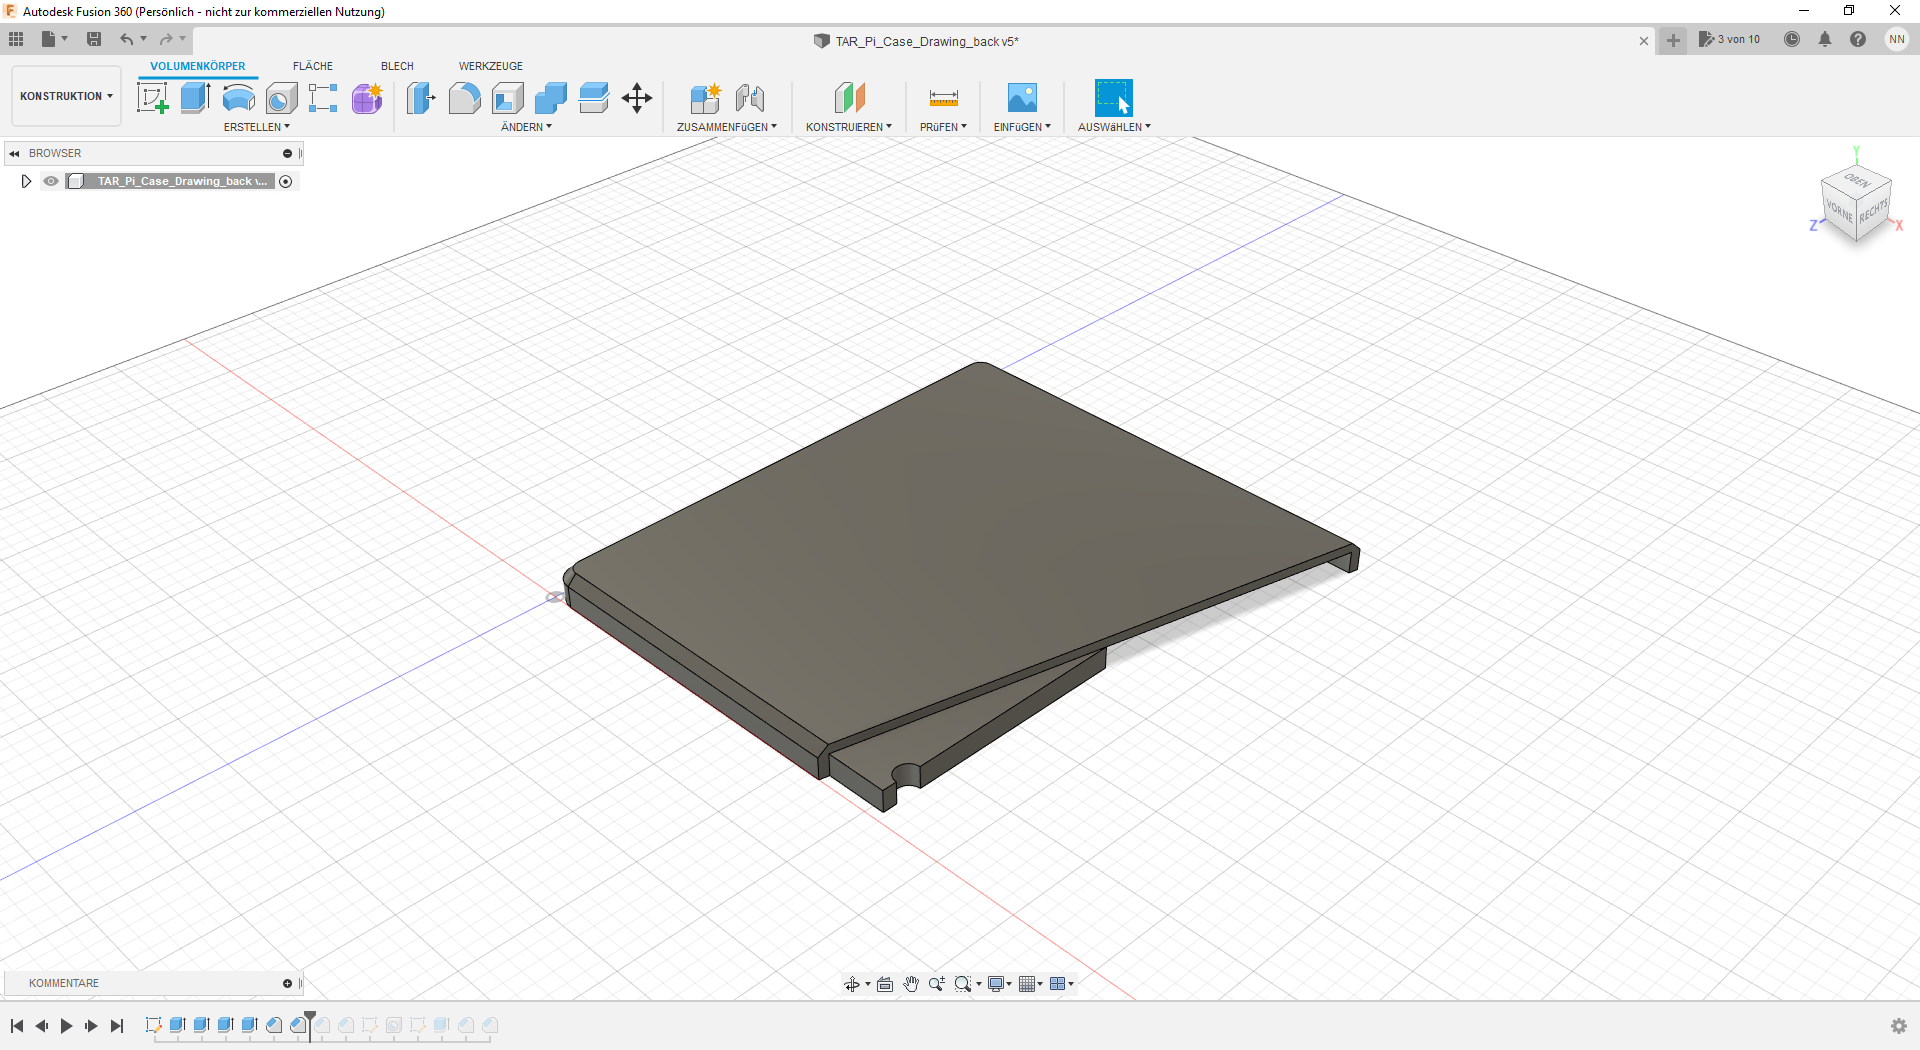
\includegraphics[width=\linewidth]{img/konstruktion_gehaeuse_hinten_007.png}
		\caption[Abfasen der Außenseite]{Abfasen der Außenseite}
		\label{fig:design-back-07}
	\end{subfigure}
	\begin{subfigure}[t]{.3\linewidth}
		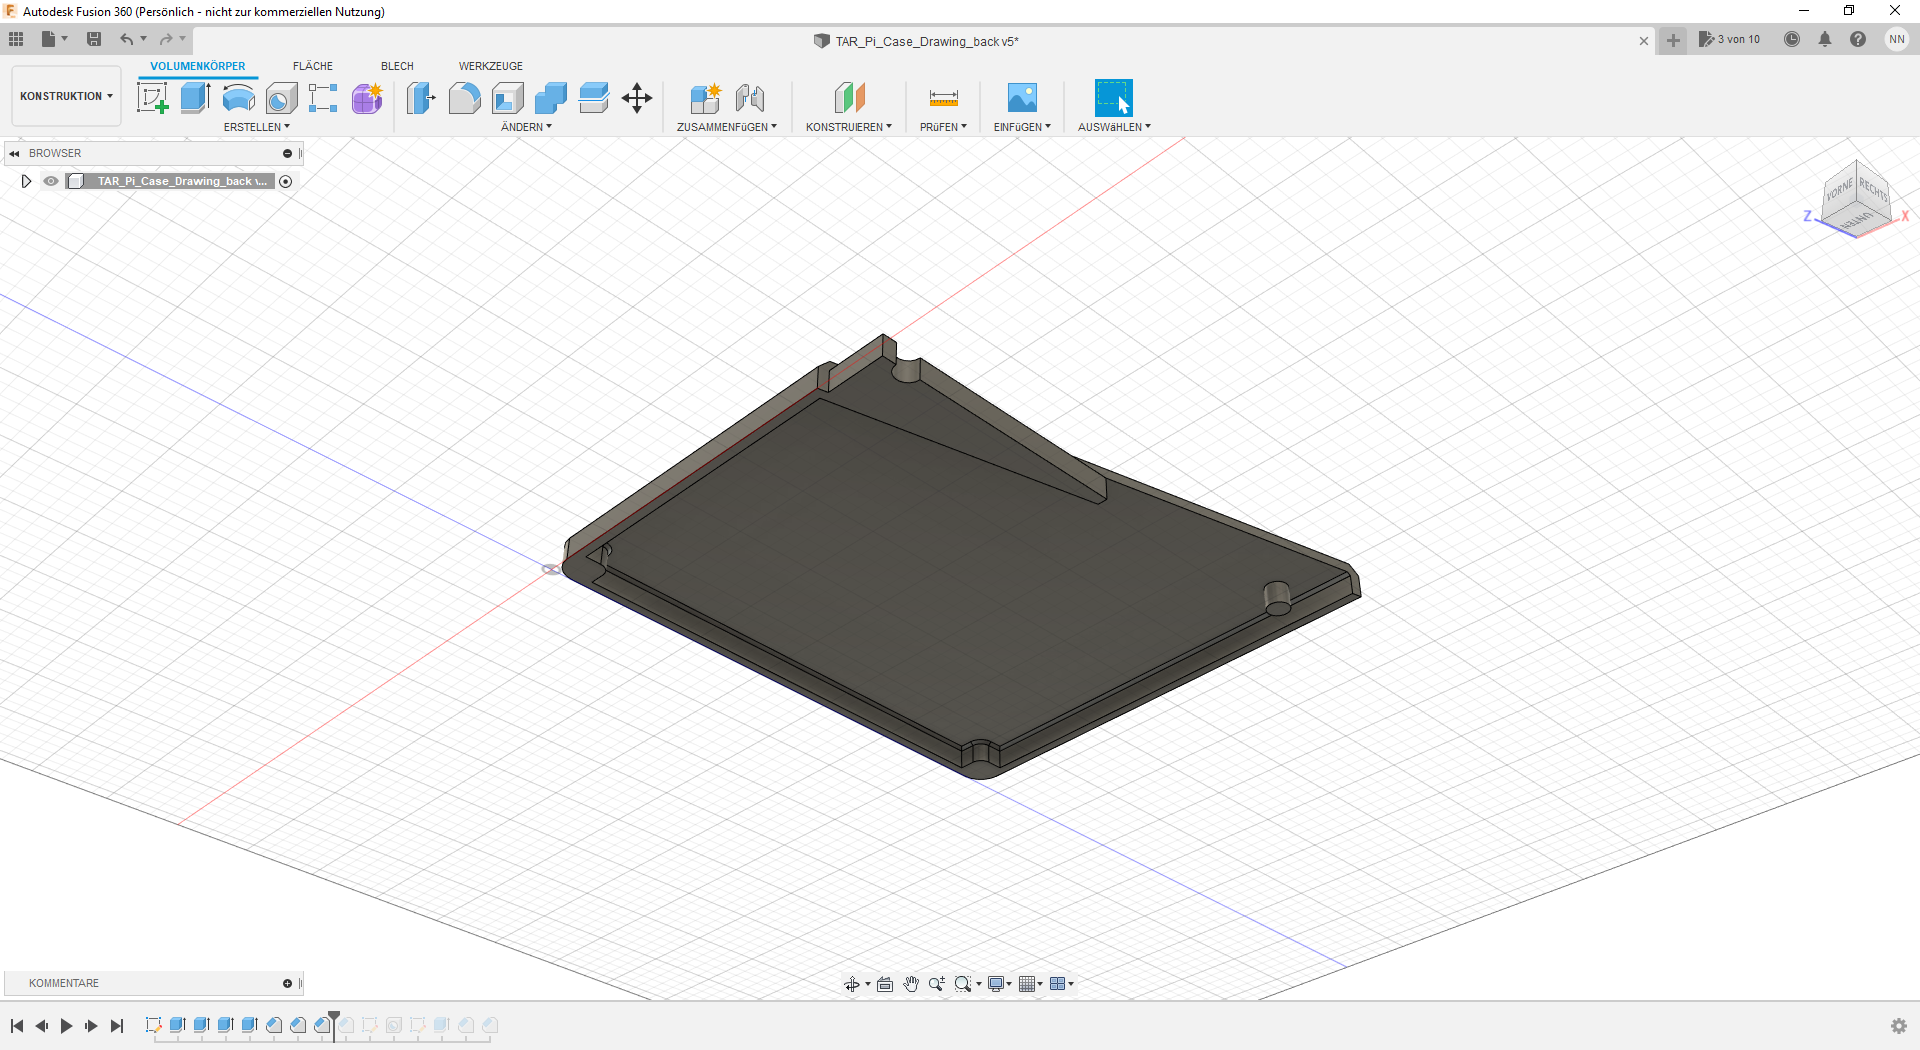
\includegraphics[width=\linewidth]{img/konstruktion_gehaeuse_hinten_008.png}
		\caption[Anbringung der Fase an der Innenseite]{Anbringung der Fase an der Innenseite}
		\label{fig:design-back-08}
	\end{subfigure}
	\begin{subfigure}[t]{.3\linewidth}
		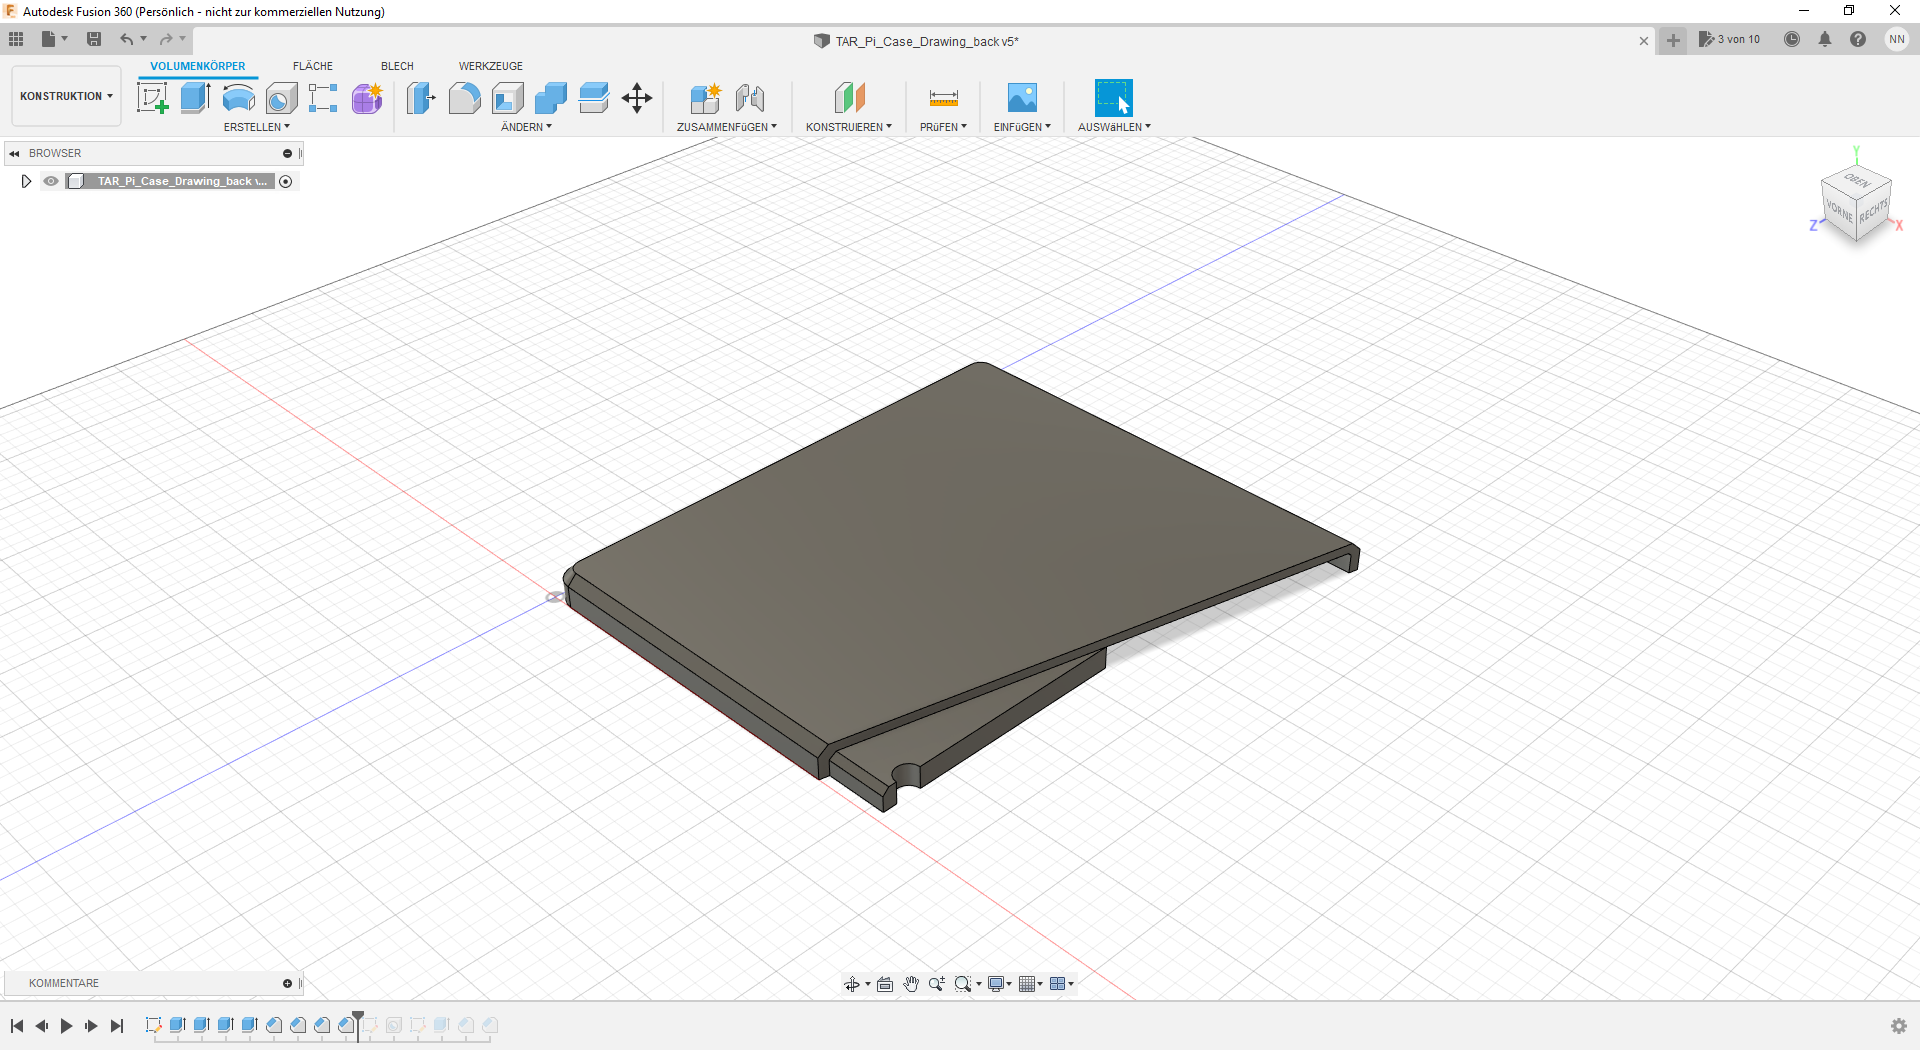
\includegraphics[width=\linewidth]{img/konstruktion_gehaeuse_hinten_009.png}
		\caption[Anbringung der Fase am Vorsprung]{Anbringung der Fase am Vorsprung}
		\label{fig:design-back-09}
	\end{subfigure}
	\begin{subfigure}[t]{.3\linewidth}
		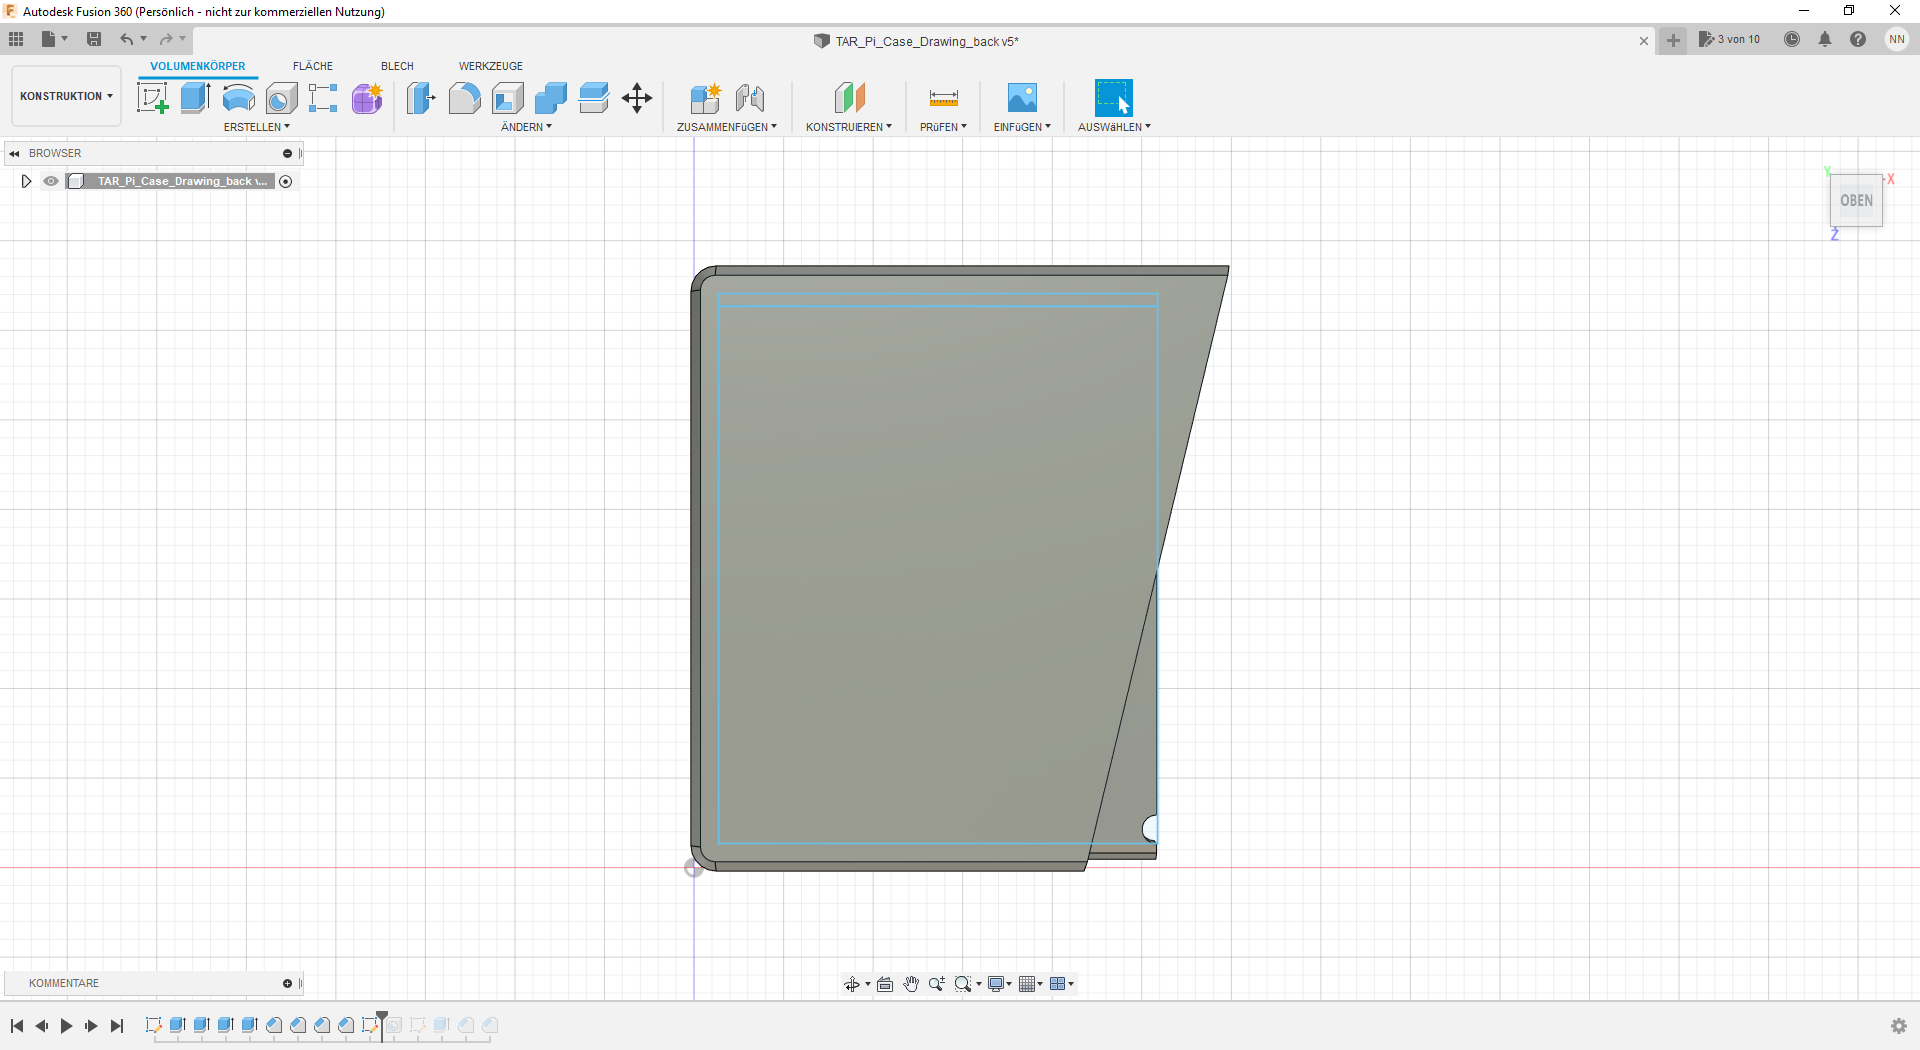
\includegraphics[width=\linewidth]{img/konstruktion_gehaeuse_hinten_010.png}
		\caption[Hilfszeichnung für Bohrungen]{Hilfszeichnung für Bohrungen}
		\label{fig:design-back-10}
	\end{subfigure}
	\begin{subfigure}[t]{.3\linewidth}
		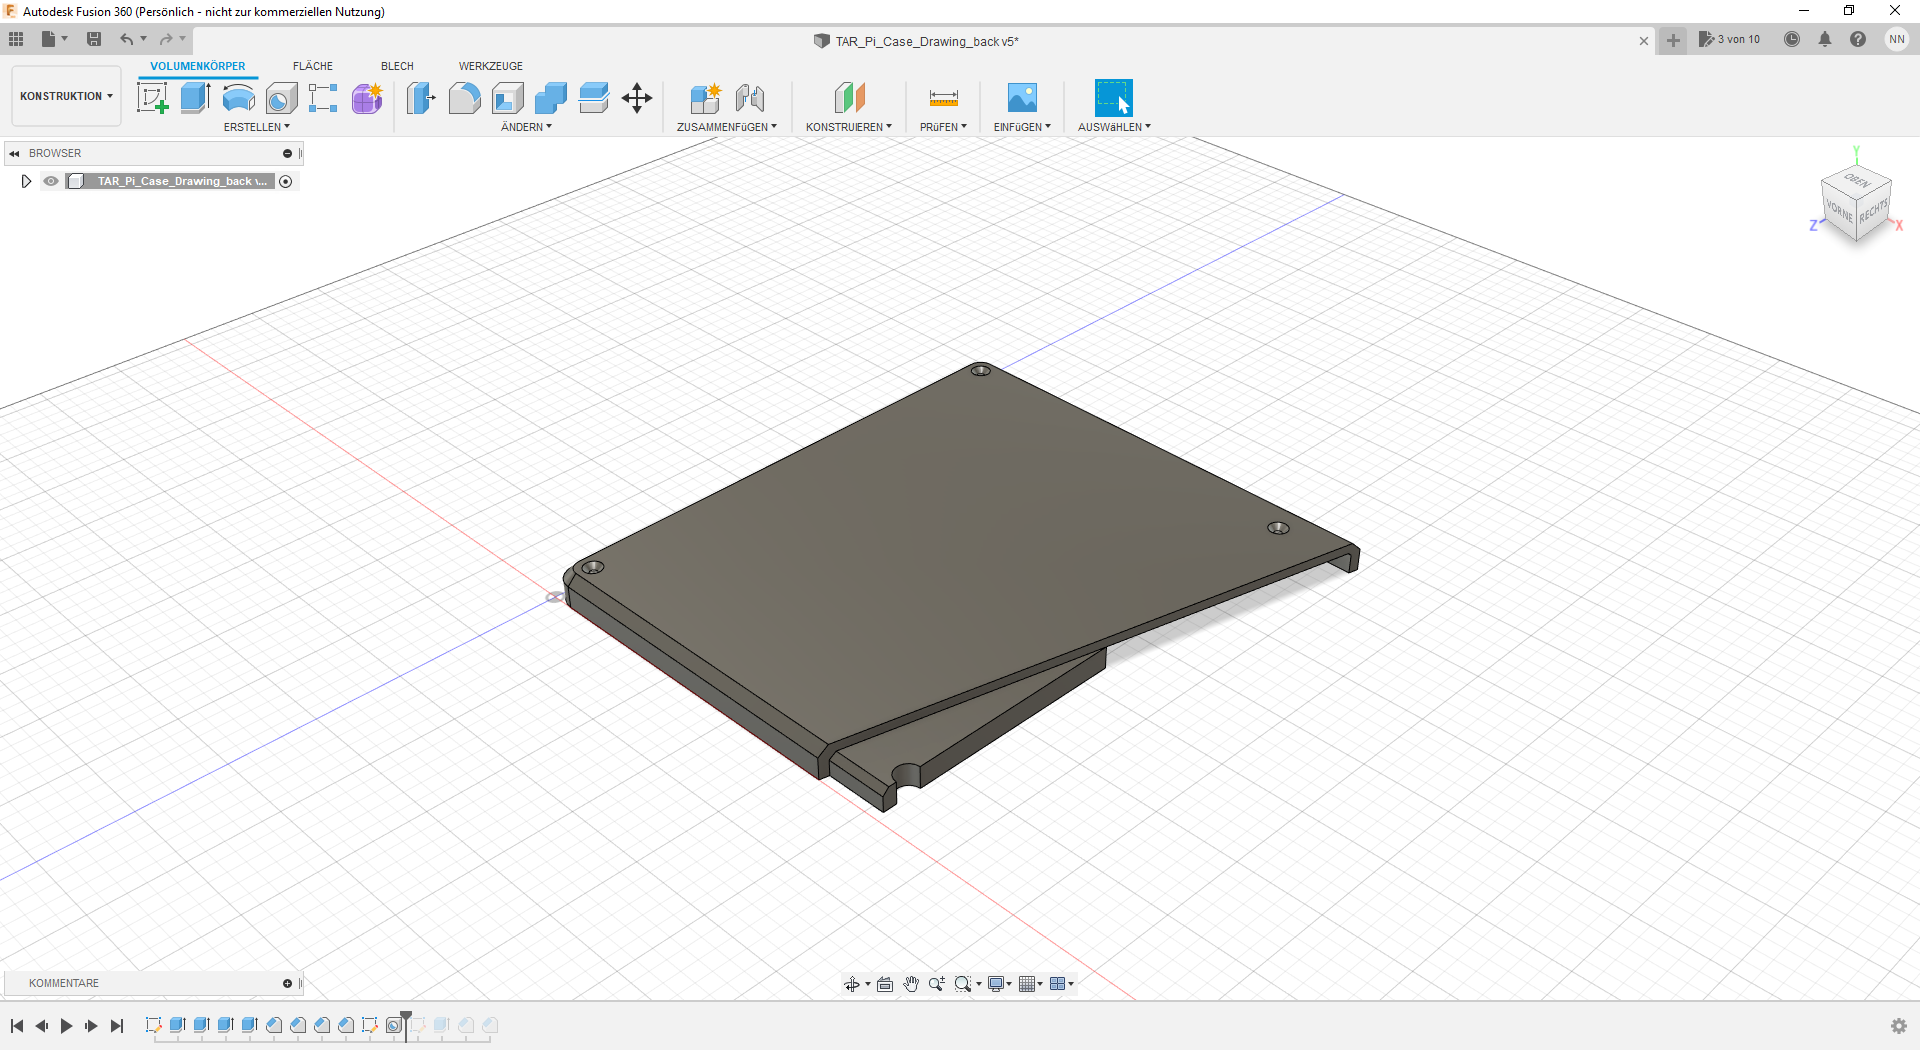
\includegraphics[width=\linewidth]{img/konstruktion_gehaeuse_hinten_011.png}
		\caption[Bohrungen mit Aussparung für Senkkopfschrauben]{Bohrungen mit Aussparung für Senkkopfschrauben}
		\label{fig:design-back-11}
	\end{subfigure}
	\begin{subfigure}[t]{.3\linewidth}
		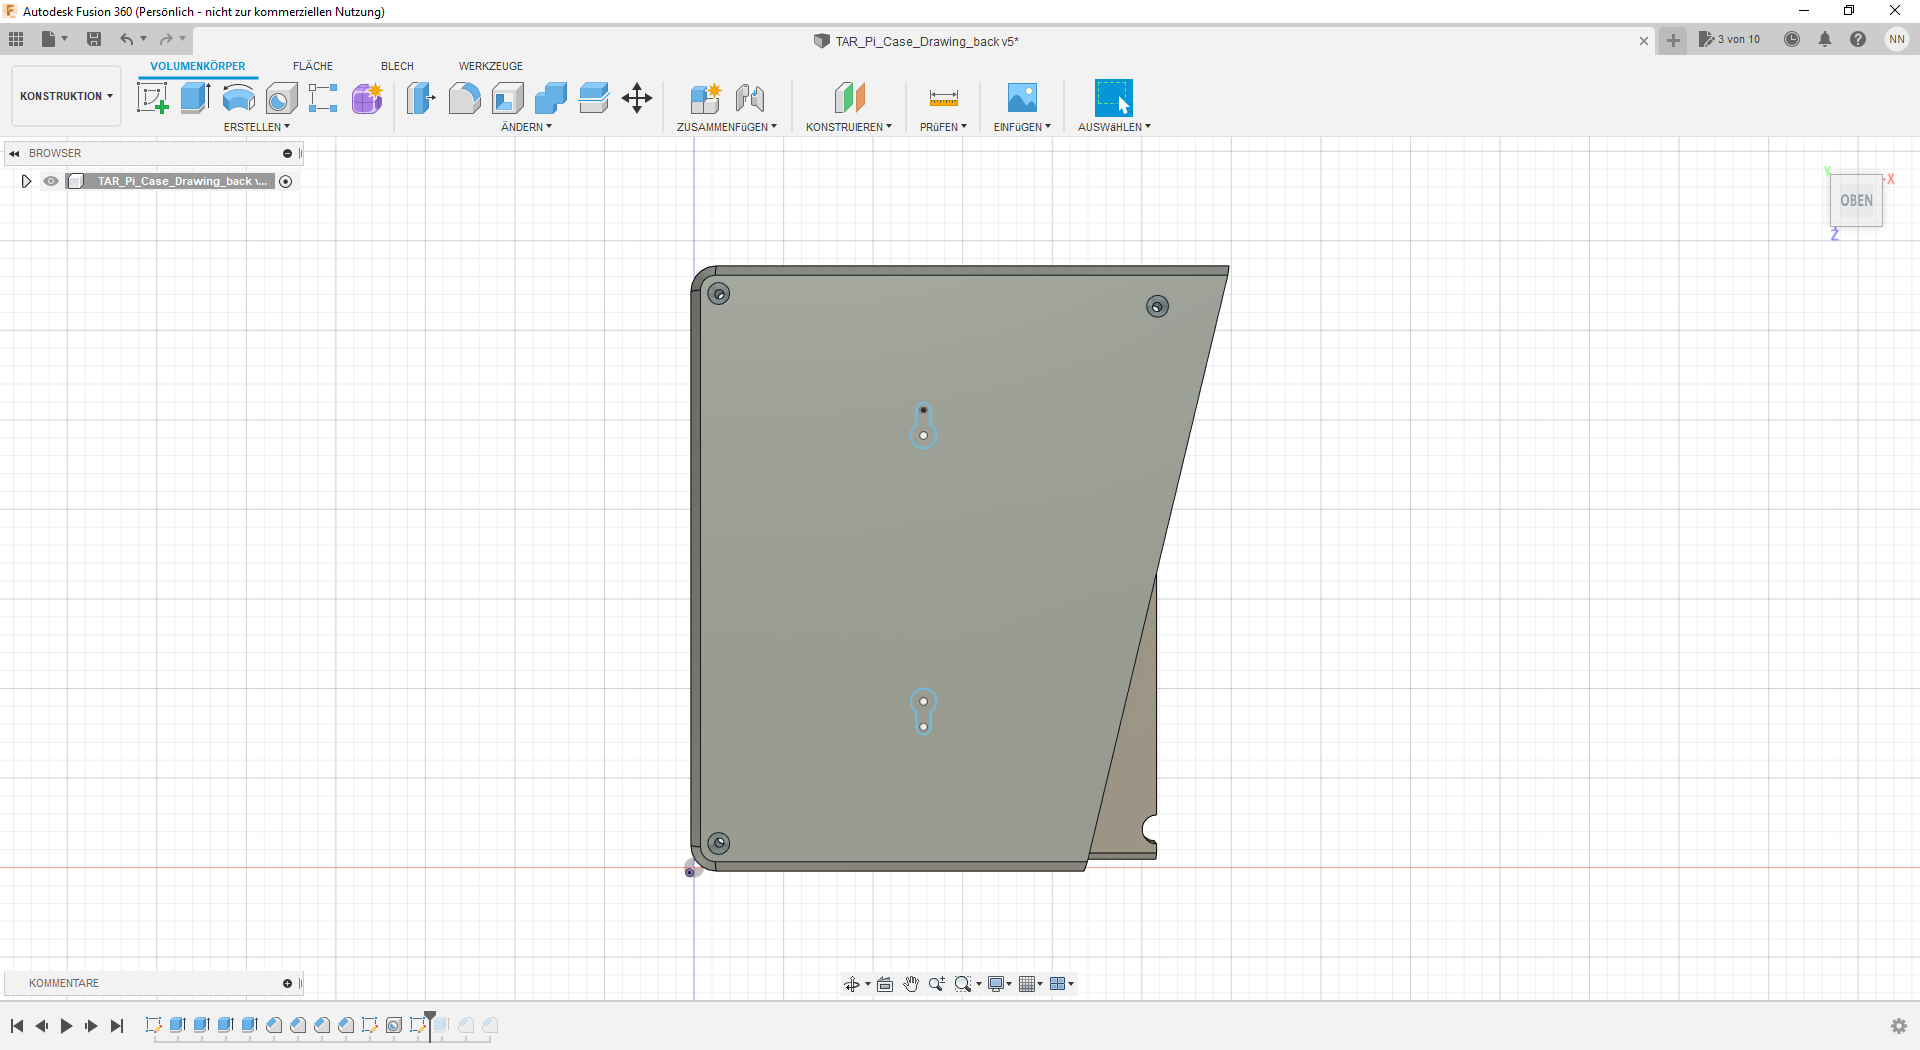
\includegraphics[width=\linewidth]{img/konstruktion_gehaeuse_hinten_012.png}
		\caption[Zeichnung für Wandaufhängungslöcher]{Zeichnung für Wandaufhängungslöcher}
		\label{fig:design-back-12}
	\end{subfigure}
	\begin{subfigure}[t]{.3\linewidth}
		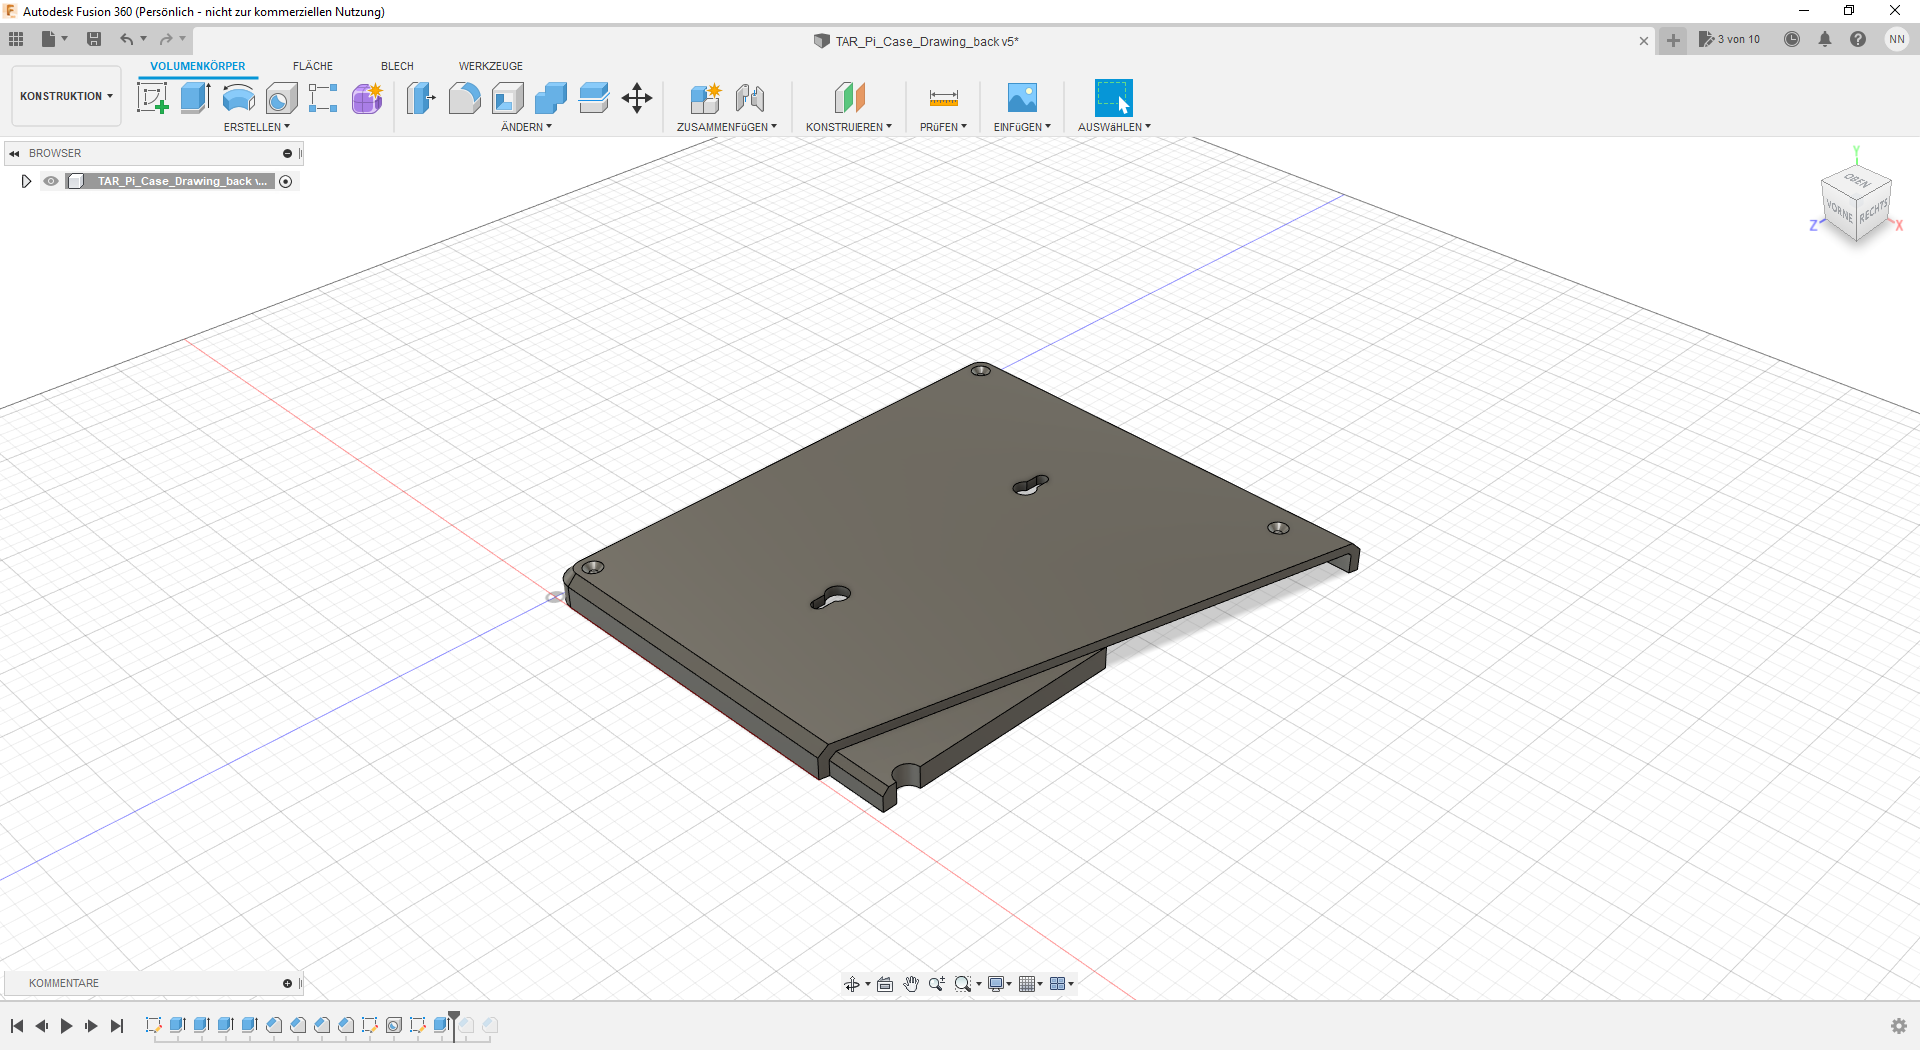
\includegraphics[width=\linewidth]{img/konstruktion_gehaeuse_hinten_013.png}
		\caption[Extrusion der Wandaufhängungslöcher]{Extrusion der Wandaufhängungslöcher}
		\label{fig:design-back-13}
	\end{subfigure}
	\begin{subfigure}[t]{.3\linewidth}
		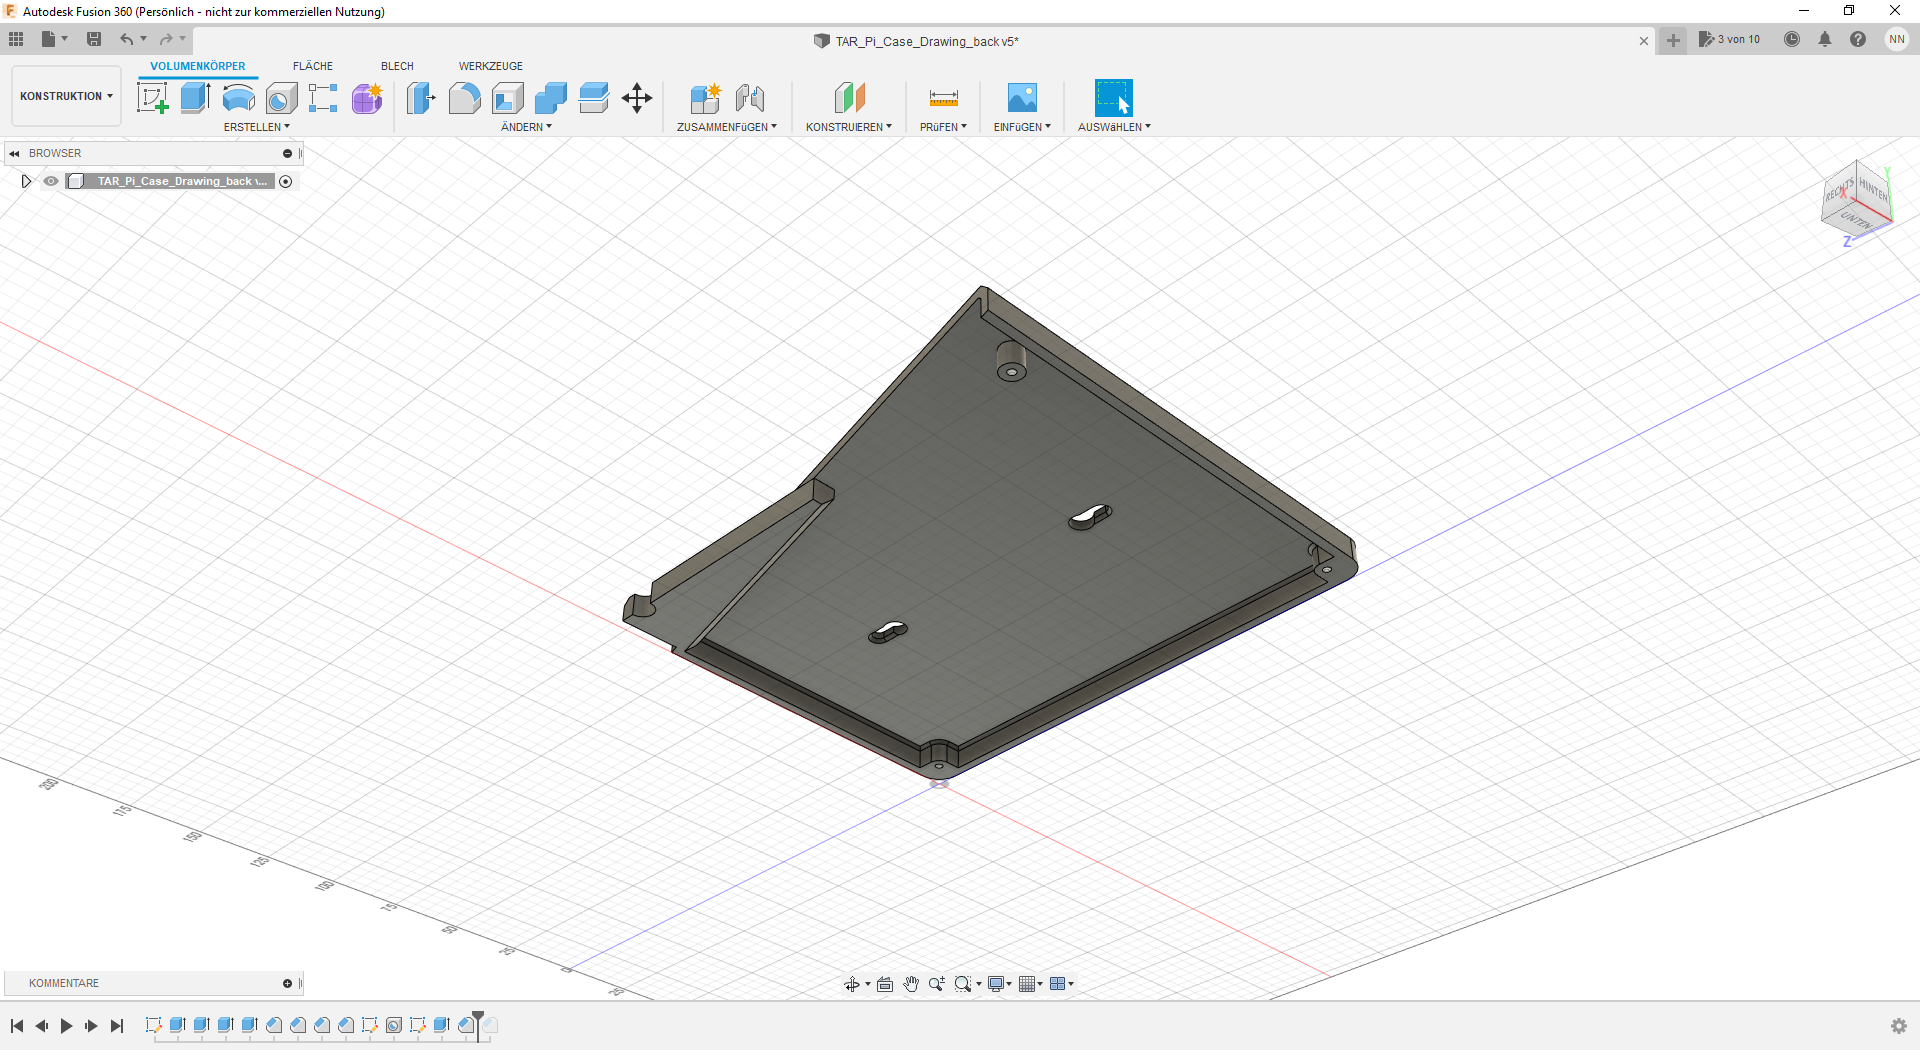
\includegraphics[width=\linewidth]{img/konstruktion_gehaeuse_hinten_014.png}
		\caption[Abfasen der Wandaufhängungslöcher]{Abfasen der Wandaufhängungslöcher}
		\label{fig:design-back-14}
	\end{subfigure}
	\begin{subfigure}[t]{.3\linewidth}
		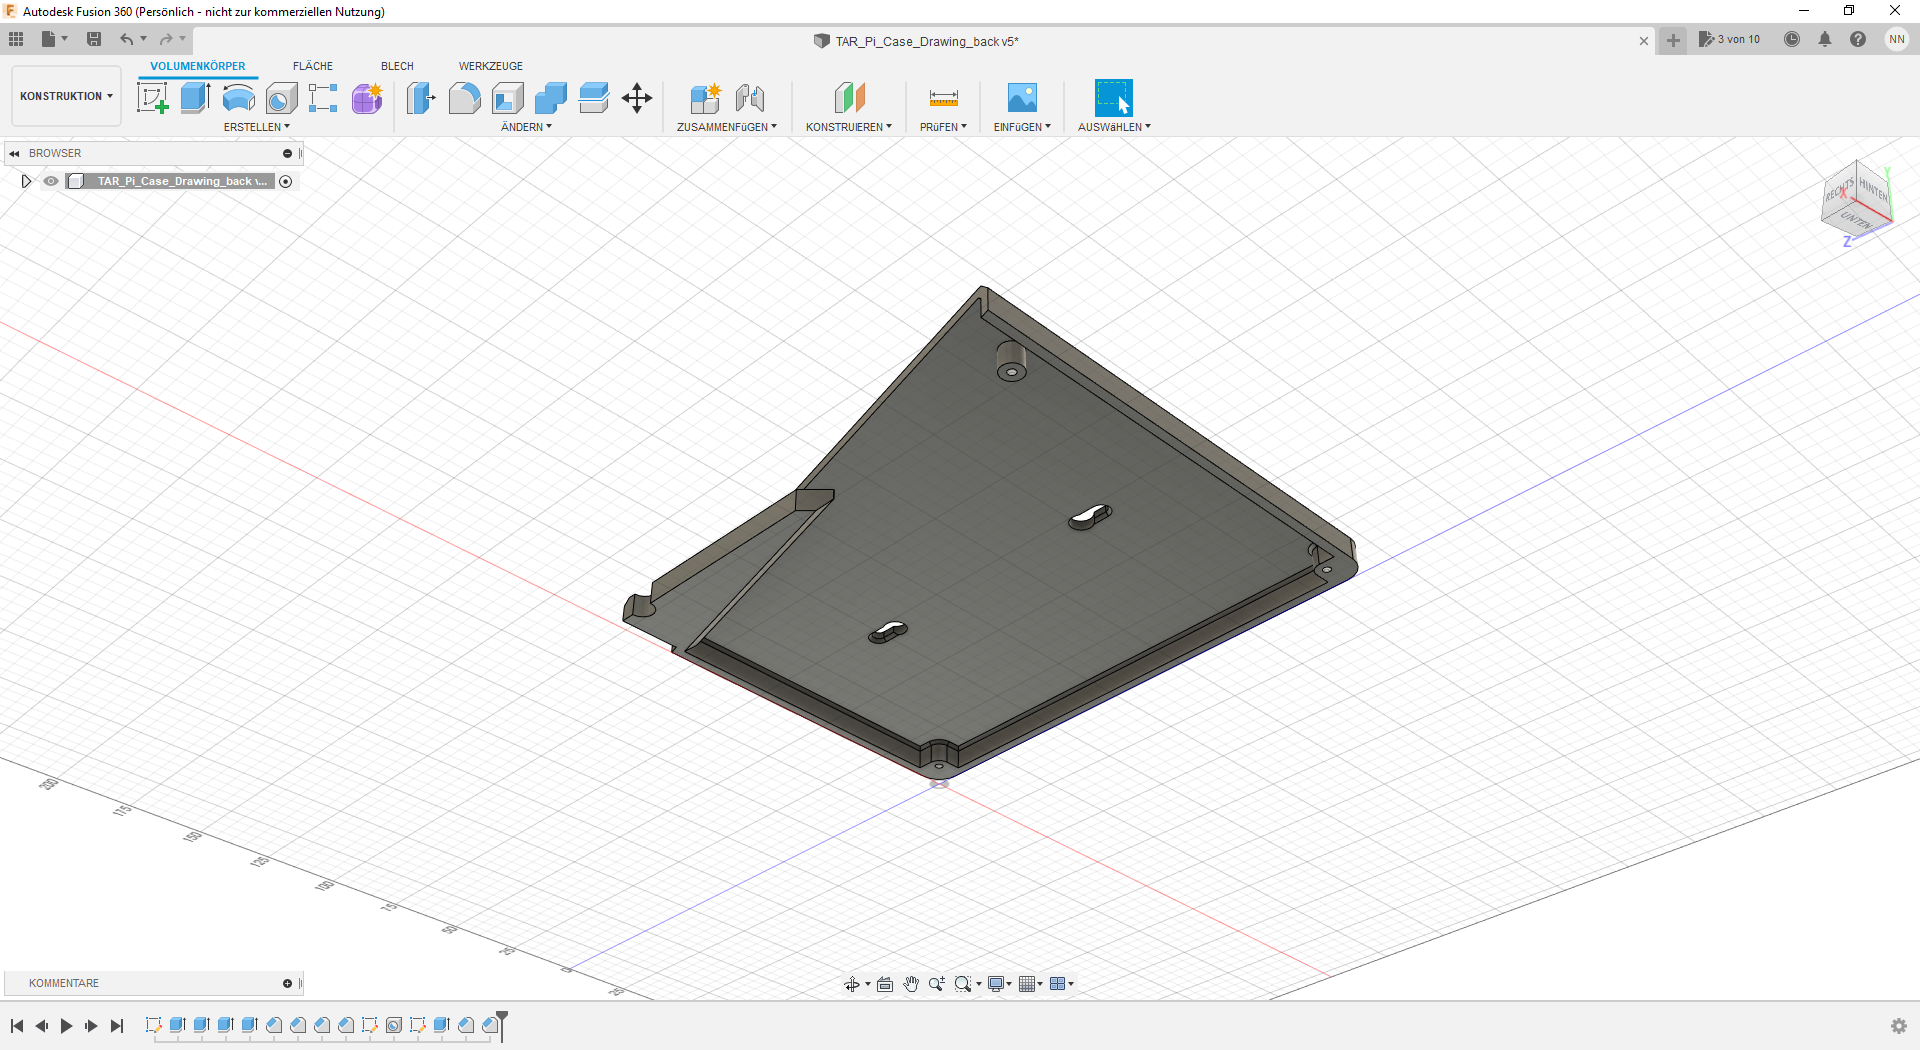
\includegraphics[width=\linewidth]{img/konstruktion_gehaeuse_hinten_015.png}
		\caption[Abfasen des Vorsprungs in der Mitte]{Abfasen des Vorsprungs in der Mitte}
		\label{fig:design-back-15}
	\end{subfigure}
	\caption[Entwurf der Gehäuserückwand]{Entwurf der Gehäuserückwand}
	\label{fig:design-back}
\end{figure}\par
\newpage